\documentclass[twoside]{book}

% Packages required by doxygen
\usepackage{calc}
\usepackage{doxygen}
\usepackage{graphicx}
\usepackage[utf8]{inputenc}
\usepackage{makeidx}
\usepackage{multicol}
\usepackage{multirow}
\usepackage{textcomp}
\usepackage[table]{xcolor}

% Font selection
\usepackage[T1]{fontenc}
\usepackage{mathptmx}
\usepackage[scaled=.90]{helvet}
\usepackage{courier}
\usepackage{amssymb}
\usepackage{sectsty}
\renewcommand{\familydefault}{\sfdefault}
\allsectionsfont{%
  \fontseries{bc}\selectfont%
  \color{darkgray}%
}
\renewcommand{\DoxyLabelFont}{%
  \fontseries{bc}\selectfont%
  \color{darkgray}%
}

% Page & text layout
\usepackage{geometry}
\geometry{%
  a4paper,%
  top=2.5cm,%
  bottom=2.5cm,%
  left=2.5cm,%
  right=2.5cm%
}
\tolerance=750
\hfuzz=15pt
\hbadness=750
\setlength{\emergencystretch}{15pt}
\setlength{\parindent}{0cm}
\setlength{\parskip}{0.2cm}
\makeatletter
\renewcommand{\paragraph}{%
  \@startsection{paragraph}{4}{0ex}{-1.0ex}{1.0ex}{%
    \normalfont\normalsize\bfseries\SS@parafont%
  }%
}
\renewcommand{\subparagraph}{%
  \@startsection{subparagraph}{5}{0ex}{-1.0ex}{1.0ex}{%
    \normalfont\normalsize\bfseries\SS@subparafont%
  }%
}
\makeatother

% Headers & footers
\usepackage{fancyhdr}
\pagestyle{fancyplain}
\fancyhead[LE]{\fancyplain{}{\bfseries\thepage}}
\fancyhead[CE]{\fancyplain{}{}}
\fancyhead[RE]{\fancyplain{}{\bfseries\leftmark}}
\fancyhead[LO]{\fancyplain{}{\bfseries\rightmark}}
\fancyhead[CO]{\fancyplain{}{}}
\fancyhead[RO]{\fancyplain{}{\bfseries\thepage}}
\fancyfoot[LE]{\fancyplain{}{}}
\fancyfoot[CE]{\fancyplain{}{}}
\fancyfoot[RE]{\fancyplain{}{\bfseries\scriptsize Generated on Wed Jan 15 2014 22\-:43\-:16 for Small\-World by Doxygen }}
\fancyfoot[LO]{\fancyplain{}{\bfseries\scriptsize Generated on Wed Jan 15 2014 22\-:43\-:16 for Small\-World by Doxygen }}
\fancyfoot[CO]{\fancyplain{}{}}
\fancyfoot[RO]{\fancyplain{}{}}
\renewcommand{\footrulewidth}{0.4pt}
\renewcommand{\chaptermark}[1]{%
  \markboth{#1}{}%
}
\renewcommand{\sectionmark}[1]{%
  \markright{\thesection\ #1}%
}

% Indices & bibliography
\usepackage{natbib}
\usepackage[titles]{tocloft}
\setcounter{tocdepth}{3}
\setcounter{secnumdepth}{5}
\makeindex

% Hyperlinks (required, but should be loaded last)
\usepackage{ifpdf}
\ifpdf
  \usepackage[pdftex,pagebackref=true]{hyperref}
\else
  \usepackage[ps2pdf,pagebackref=true]{hyperref}
\fi
\hypersetup{%
  colorlinks=true,%
  linkcolor=blue,%
  citecolor=blue,%
  unicode%
}

% Custom commands
\newcommand{\clearemptydoublepage}{%
  \newpage{\pagestyle{empty}\cleardoublepage}%
}


%===== C O N T E N T S =====

\begin{document}

% Titlepage & ToC
\hypersetup{pageanchor=false}
\pagenumbering{roman}
\begin{titlepage}
\vspace*{7cm}
\begin{center}%
{\Large Small\-World }\\
\vspace*{1cm}
{\large Generated by Doxygen 1.8.5}\\
\vspace*{0.5cm}
{\small Wed Jan 15 2014 22:43:16}\\
\end{center}
\end{titlepage}
\clearemptydoublepage
\tableofcontents
\clearemptydoublepage
\pagenumbering{arabic}
\hypersetup{pageanchor=true}

%--- Begin generated contents ---
\chapter{Namespace Index}
\section{Packages}
Here are the packages with brief descriptions (if available)\-:\begin{DoxyCompactList}
\item\contentsline{section}{\hyperlink{namespace_small_world}{Small\-World} }{\pageref{namespace_small_world}}{}
\item\contentsline{section}{\hyperlink{namespace_small_world_1_1_properties}{Small\-World.\-Properties} }{\pageref{namespace_small_world_1_1_properties}}{}
\end{DoxyCompactList}

\chapter{Hierarchical Index}
\section{Class Hierarchy}
This inheritance list is sorted roughly, but not completely, alphabetically\-:\begin{DoxyCompactList}
\item \contentsline{section}{Small\-World.\-Constantes}{\pageref{class_small_world_1_1_constantes}}{}
\item \contentsline{section}{Small\-World.\-Inter\-Carte}{\pageref{interface_small_world_1_1_inter_carte}}{}
\begin{DoxyCompactList}
\item \contentsline{section}{Small\-World.\-Carte}{\pageref{class_small_world_1_1_carte}}{}
\end{DoxyCompactList}
\item \contentsline{section}{Small\-World.\-Inter\-Case}{\pageref{interface_small_world_1_1_inter_case}}{}
\begin{DoxyCompactList}
\item \contentsline{section}{Small\-World.\-Case}{\pageref{class_small_world_1_1_case}}{}
\begin{DoxyCompactList}
\item \contentsline{section}{Small\-World.\-Desert}{\pageref{class_small_world_1_1_desert}}{}
\item \contentsline{section}{Small\-World.\-Eau}{\pageref{class_small_world_1_1_eau}}{}
\item \contentsline{section}{Small\-World.\-Foret}{\pageref{class_small_world_1_1_foret}}{}
\item \contentsline{section}{Small\-World.\-Montagne}{\pageref{class_small_world_1_1_montagne}}{}
\item \contentsline{section}{Small\-World.\-Plaine}{\pageref{class_small_world_1_1_plaine}}{}
\end{DoxyCompactList}
\item \contentsline{section}{Small\-World.\-Inter\-Desert}{\pageref{interface_small_world_1_1_inter_desert}}{}
\begin{DoxyCompactList}
\item \contentsline{section}{Small\-World.\-Desert}{\pageref{class_small_world_1_1_desert}}{}
\end{DoxyCompactList}
\item \contentsline{section}{Small\-World.\-Inter\-Eau}{\pageref{interface_small_world_1_1_inter_eau}}{}
\begin{DoxyCompactList}
\item \contentsline{section}{Small\-World.\-Eau}{\pageref{class_small_world_1_1_eau}}{}
\end{DoxyCompactList}
\item \contentsline{section}{Small\-World.\-Inter\-Foret}{\pageref{interface_small_world_1_1_inter_foret}}{}
\begin{DoxyCompactList}
\item \contentsline{section}{Small\-World.\-Foret}{\pageref{class_small_world_1_1_foret}}{}
\end{DoxyCompactList}
\item \contentsline{section}{Small\-World.\-Inter\-Montagne}{\pageref{interface_small_world_1_1_inter_montagne}}{}
\begin{DoxyCompactList}
\item \contentsline{section}{Small\-World.\-Montagne}{\pageref{class_small_world_1_1_montagne}}{}
\end{DoxyCompactList}
\item \contentsline{section}{Small\-World.\-Inter\-Plaine}{\pageref{interface_small_world_1_1_inter_plaine}}{}
\begin{DoxyCompactList}
\item \contentsline{section}{Small\-World.\-Plaine}{\pageref{class_small_world_1_1_plaine}}{}
\end{DoxyCompactList}
\end{DoxyCompactList}
\item \contentsline{section}{Inter\-Coordonnees}{\pageref{interface_inter_coordonnees}}{}
\item \contentsline{section}{Small\-World.\-Inter\-Cordonnees}{\pageref{interface_small_world_1_1_inter_cordonnees}}{}
\begin{DoxyCompactList}
\item \contentsline{section}{Small\-World.\-Coordonnees}{\pageref{class_small_world_1_1_coordonnees}}{}
\end{DoxyCompactList}
\item \contentsline{section}{Small\-World.\-Inter\-Createur\-Partie}{\pageref{interface_small_world_1_1_inter_createur_partie}}{}
\begin{DoxyCompactList}
\item \contentsline{section}{Small\-World.\-Createur\-Partie}{\pageref{class_small_world_1_1_createur_partie}}{}
\end{DoxyCompactList}
\item \contentsline{section}{Small\-World.\-Inter\-Fabrique\-Case}{\pageref{interface_small_world_1_1_inter_fabrique_case}}{}
\begin{DoxyCompactList}
\item \contentsline{section}{Small\-World.\-Fabrique\-Case}{\pageref{class_small_world_1_1_fabrique_case}}{}
\end{DoxyCompactList}
\item \contentsline{section}{Small\-World.\-Inter\-Fabrique\-Peuple}{\pageref{interface_small_world_1_1_inter_fabrique_peuple}}{}
\begin{DoxyCompactList}
\item \contentsline{section}{Small\-World.\-Fabrique\-Peuple}{\pageref{class_small_world_1_1_fabrique_peuple}}{}
\end{DoxyCompactList}
\item \contentsline{section}{Small\-World.\-Inter\-Joueur}{\pageref{interface_small_world_1_1_inter_joueur}}{}
\begin{DoxyCompactList}
\item \contentsline{section}{Small\-World.\-Joueur}{\pageref{class_small_world_1_1_joueur}}{}
\end{DoxyCompactList}
\item \contentsline{section}{Small\-World.\-Inter\-Monteur\-Partie}{\pageref{interface_small_world_1_1_inter_monteur_partie}}{}
\begin{DoxyCompactList}
\item \contentsline{section}{Small\-World.\-Inter\-Monteur\-Partie\-Demo}{\pageref{interface_small_world_1_1_inter_monteur_partie_demo}}{}
\begin{DoxyCompactList}
\item \contentsline{section}{Small\-World.\-Monteur\-Partie\-Demo}{\pageref{class_small_world_1_1_monteur_partie_demo}}{}
\end{DoxyCompactList}
\item \contentsline{section}{Small\-World.\-Inter\-Monteur\-Partie\-Normale}{\pageref{interface_small_world_1_1_inter_monteur_partie_normale}}{}
\begin{DoxyCompactList}
\item \contentsline{section}{Small\-World.\-Monteur\-Partie\-Normale}{\pageref{class_small_world_1_1_monteur_partie_normale}}{}
\end{DoxyCompactList}
\item \contentsline{section}{Small\-World.\-Inter\-Monteur\-Partie\-Petite}{\pageref{interface_small_world_1_1_inter_monteur_partie_petite}}{}
\begin{DoxyCompactList}
\item \contentsline{section}{Small\-World.\-Monteur\-Partie\-Petite}{\pageref{class_small_world_1_1_monteur_partie_petite}}{}
\end{DoxyCompactList}
\item \contentsline{section}{Small\-World.\-Monteur\-Partie}{\pageref{class_small_world_1_1_monteur_partie}}{}
\begin{DoxyCompactList}
\item \contentsline{section}{Small\-World.\-Monteur\-Partie\-Demo}{\pageref{class_small_world_1_1_monteur_partie_demo}}{}
\item \contentsline{section}{Small\-World.\-Monteur\-Partie\-Normale}{\pageref{class_small_world_1_1_monteur_partie_normale}}{}
\item \contentsline{section}{Small\-World.\-Monteur\-Partie\-Petite}{\pageref{class_small_world_1_1_monteur_partie_petite}}{}
\end{DoxyCompactList}
\end{DoxyCompactList}
\item \contentsline{section}{Small\-World.\-Inter\-Partie}{\pageref{interface_small_world_1_1_inter_partie}}{}
\begin{DoxyCompactList}
\item \contentsline{section}{Small\-World.\-Partie}{\pageref{class_small_world_1_1_partie}}{}
\end{DoxyCompactList}
\item \contentsline{section}{Small\-World.\-Inter\-Peuple}{\pageref{interface_small_world_1_1_inter_peuple}}{}
\begin{DoxyCompactList}
\item \contentsline{section}{Small\-World.\-Inter\-Peuple\-Gaulois}{\pageref{interface_small_world_1_1_inter_peuple_gaulois}}{}
\begin{DoxyCompactList}
\item \contentsline{section}{Small\-World.\-Peuple\-Gaulois}{\pageref{class_small_world_1_1_peuple_gaulois}}{}
\end{DoxyCompactList}
\item \contentsline{section}{Small\-World.\-Inter\-Peuple\-Nain}{\pageref{interface_small_world_1_1_inter_peuple_nain}}{}
\begin{DoxyCompactList}
\item \contentsline{section}{Small\-World.\-Peuple\-Nain}{\pageref{class_small_world_1_1_peuple_nain}}{}
\end{DoxyCompactList}
\item \contentsline{section}{Small\-World.\-Inter\-Peuple\-Viking}{\pageref{interface_small_world_1_1_inter_peuple_viking}}{}
\begin{DoxyCompactList}
\item \contentsline{section}{Small\-World.\-Peuple\-Viking}{\pageref{class_small_world_1_1_peuple_viking}}{}
\end{DoxyCompactList}
\item \contentsline{section}{Small\-World.\-Peuple}{\pageref{class_small_world_1_1_peuple}}{}
\begin{DoxyCompactList}
\item \contentsline{section}{Small\-World.\-Peuple\-Gaulois}{\pageref{class_small_world_1_1_peuple_gaulois}}{}
\item \contentsline{section}{Small\-World.\-Peuple\-Nain}{\pageref{class_small_world_1_1_peuple_nain}}{}
\item \contentsline{section}{Small\-World.\-Peuple\-Viking}{\pageref{class_small_world_1_1_peuple_viking}}{}
\end{DoxyCompactList}
\end{DoxyCompactList}
\item \contentsline{section}{Small\-World.\-Inter\-Strategie\-Carte}{\pageref{interface_small_world_1_1_inter_strategie_carte}}{}
\begin{DoxyCompactList}
\item \contentsline{section}{Small\-World.\-Inter\-Strategie\-Demo}{\pageref{interface_small_world_1_1_inter_strategie_demo}}{}
\begin{DoxyCompactList}
\item \contentsline{section}{Small\-World.\-Strategie\-Demo}{\pageref{class_small_world_1_1_strategie_demo}}{}
\end{DoxyCompactList}
\item \contentsline{section}{Small\-World.\-Inter\-Strategie\-Normale}{\pageref{interface_small_world_1_1_inter_strategie_normale}}{}
\begin{DoxyCompactList}
\item \contentsline{section}{Small\-World.\-Strategie\-Normale}{\pageref{class_small_world_1_1_strategie_normale}}{}
\end{DoxyCompactList}
\item \contentsline{section}{Small\-World.\-Inter\-Strategie\-Petite}{\pageref{interface_small_world_1_1_inter_strategie_petite}}{}
\begin{DoxyCompactList}
\item \contentsline{section}{Small\-World.\-Strategie\-Petite}{\pageref{class_small_world_1_1_strategie_petite}}{}
\end{DoxyCompactList}
\item \contentsline{section}{Small\-World.\-Strategie\-Carte}{\pageref{class_small_world_1_1_strategie_carte}}{}
\begin{DoxyCompactList}
\item \contentsline{section}{Small\-World.\-Strategie\-Demo}{\pageref{class_small_world_1_1_strategie_demo}}{}
\item \contentsline{section}{Small\-World.\-Strategie\-Normale}{\pageref{class_small_world_1_1_strategie_normale}}{}
\item \contentsline{section}{Small\-World.\-Strategie\-Petite}{\pageref{class_small_world_1_1_strategie_petite}}{}
\end{DoxyCompactList}
\end{DoxyCompactList}
\item \contentsline{section}{Small\-World.\-Inter\-Unite}{\pageref{interface_small_world_1_1_inter_unite}}{}
\begin{DoxyCompactList}
\item \contentsline{section}{Small\-World.\-Inter\-Unite\-Gauloise}{\pageref{interface_small_world_1_1_inter_unite_gauloise}}{}
\begin{DoxyCompactList}
\item \contentsline{section}{Small\-World.\-Unite\-Gauloise}{\pageref{class_small_world_1_1_unite_gauloise}}{}
\end{DoxyCompactList}
\item \contentsline{section}{Small\-World.\-Inter\-Unite\-Naine}{\pageref{interface_small_world_1_1_inter_unite_naine}}{}
\begin{DoxyCompactList}
\item \contentsline{section}{Small\-World.\-Unite\-Naine}{\pageref{class_small_world_1_1_unite_naine}}{}
\end{DoxyCompactList}
\item \contentsline{section}{Small\-World.\-Inter\-Unite\-Viking}{\pageref{interface_small_world_1_1_inter_unite_viking}}{}
\begin{DoxyCompactList}
\item \contentsline{section}{Small\-World.\-Unite\-Viking}{\pageref{class_small_world_1_1_unite_viking}}{}
\end{DoxyCompactList}
\item \contentsline{section}{Small\-World.\-Unite}{\pageref{class_small_world_1_1_unite}}{}
\begin{DoxyCompactList}
\item \contentsline{section}{Small\-World.\-Unite\-Gauloise}{\pageref{class_small_world_1_1_unite_gauloise}}{}
\item \contentsline{section}{Small\-World.\-Unite\-Naine}{\pageref{class_small_world_1_1_unite_naine}}{}
\item \contentsline{section}{Small\-World.\-Unite\-Viking}{\pageref{class_small_world_1_1_unite_viking}}{}
\end{DoxyCompactList}
\end{DoxyCompactList}
\end{DoxyCompactList}

\chapter{Class Index}
\section{Class List}
Here are the classes, structs, unions and interfaces with brief descriptions\-:\begin{DoxyCompactList}
\item\contentsline{section}{\hyperlink{class_small_world_1_1_carte}{Small\-World.\-Carte} }{\pageref{class_small_world_1_1_carte}}{}
\item\contentsline{section}{\hyperlink{class_small_world_1_1_case}{Small\-World.\-Case} }{\pageref{class_small_world_1_1_case}}{}
\item\contentsline{section}{\hyperlink{class_small_world_1_1_createur_partie}{Small\-World.\-Createur\-Partie} \\*Class du créateur de partie }{\pageref{class_small_world_1_1_createur_partie}}{}
\item\contentsline{section}{\hyperlink{class_small_world_1_1_desert}{Small\-World.\-Desert} }{\pageref{class_small_world_1_1_desert}}{}
\item\contentsline{section}{\hyperlink{class_small_world_1_1_eau}{Small\-World.\-Eau} }{\pageref{class_small_world_1_1_eau}}{}
\item\contentsline{section}{\hyperlink{interface_small_world_1_1_fabrique___unite___gaulois}{Small\-World.\-Fabrique\-\_\-\-Unite\-\_\-\-Gaulois} }{\pageref{interface_small_world_1_1_fabrique___unite___gaulois}}{}
\item\contentsline{section}{\hyperlink{interface_small_world_1_1_fabrique___unite___nain}{Small\-World.\-Fabrique\-\_\-\-Unite\-\_\-\-Nain} }{\pageref{interface_small_world_1_1_fabrique___unite___nain}}{}
\item\contentsline{section}{\hyperlink{interface_small_world_1_1_fabrique___unite___viking}{Small\-World.\-Fabrique\-\_\-\-Unite\-\_\-\-Viking} }{\pageref{interface_small_world_1_1_fabrique___unite___viking}}{}
\item\contentsline{section}{\hyperlink{class_small_world_1_1_fabrique_case}{Small\-World.\-Fabrique\-Case} }{\pageref{class_small_world_1_1_fabrique_case}}{}
\item\contentsline{section}{\hyperlink{interface_small_world_1_1_fabrique_jeu}{Small\-World.\-Fabrique\-Jeu} }{\pageref{interface_small_world_1_1_fabrique_jeu}}{}
\item\contentsline{section}{\hyperlink{class_small_world_1_1_fabrique_peuple}{Small\-World.\-Fabrique\-Peuple} }{\pageref{class_small_world_1_1_fabrique_peuple}}{}
\item\contentsline{section}{\hyperlink{class_small_world_1_1_foret}{Small\-World.\-Foret} }{\pageref{class_small_world_1_1_foret}}{}
\item\contentsline{section}{\hyperlink{interface_small_world_1_1_inter_carte}{Small\-World.\-Inter\-Carte} }{\pageref{interface_small_world_1_1_inter_carte}}{}
\item\contentsline{section}{\hyperlink{interface_small_world_1_1_inter_case}{Small\-World.\-Inter\-Case} }{\pageref{interface_small_world_1_1_inter_case}}{}
\item\contentsline{section}{\hyperlink{interface_small_world_1_1_inter_createur_partie}{Small\-World.\-Inter\-Createur\-Partie} \\*Interface du créateur de partie }{\pageref{interface_small_world_1_1_inter_createur_partie}}{}
\item\contentsline{section}{\hyperlink{interface_small_world_1_1_inter_desert}{Small\-World.\-Inter\-Desert} }{\pageref{interface_small_world_1_1_inter_desert}}{}
\item\contentsline{section}{\hyperlink{interface_small_world_1_1_inter_eau}{Small\-World.\-Inter\-Eau} }{\pageref{interface_small_world_1_1_inter_eau}}{}
\item\contentsline{section}{\hyperlink{interface_small_world_1_1_inter_fabrique_case}{Small\-World.\-Inter\-Fabrique\-Case} }{\pageref{interface_small_world_1_1_inter_fabrique_case}}{}
\item\contentsline{section}{\hyperlink{interface_small_world_1_1_inter_fabrique_peuple}{Small\-World.\-Inter\-Fabrique\-Peuple} }{\pageref{interface_small_world_1_1_inter_fabrique_peuple}}{}
\item\contentsline{section}{\hyperlink{interface_small_world_1_1_inter_foret}{Small\-World.\-Inter\-Foret} }{\pageref{interface_small_world_1_1_inter_foret}}{}
\item\contentsline{section}{\hyperlink{interface_small_world_1_1_inter_montagne}{Small\-World.\-Inter\-Montagne} }{\pageref{interface_small_world_1_1_inter_montagne}}{}
\item\contentsline{section}{\hyperlink{interface_small_world_1_1_inter_monteur_partie}{Small\-World.\-Inter\-Monteur\-Partie} \\*Interface globale du monteur }{\pageref{interface_small_world_1_1_inter_monteur_partie}}{}
\item\contentsline{section}{\hyperlink{interface_small_world_1_1_inter_monteur_partie_demo}{Small\-World.\-Inter\-Monteur\-Partie\-Demo} }{\pageref{interface_small_world_1_1_inter_monteur_partie_demo}}{}
\item\contentsline{section}{\hyperlink{interface_small_world_1_1_inter_monteur_partie_normale}{Small\-World.\-Inter\-Monteur\-Partie\-Normale} }{\pageref{interface_small_world_1_1_inter_monteur_partie_normale}}{}
\item\contentsline{section}{\hyperlink{interface_small_world_1_1_inter_monteur_partie_petite}{Small\-World.\-Inter\-Monteur\-Partie\-Petite} }{\pageref{interface_small_world_1_1_inter_monteur_partie_petite}}{}
\item\contentsline{section}{\hyperlink{interface_small_world_1_1_inter_peuple}{Small\-World.\-Inter\-Peuple} }{\pageref{interface_small_world_1_1_inter_peuple}}{}
\item\contentsline{section}{\hyperlink{interface_small_world_1_1_inter_peuple_gaulois}{Small\-World.\-Inter\-Peuple\-Gaulois} }{\pageref{interface_small_world_1_1_inter_peuple_gaulois}}{}
\item\contentsline{section}{\hyperlink{interface_small_world_1_1_inter_peuple_nain}{Small\-World.\-Inter\-Peuple\-Nain} }{\pageref{interface_small_world_1_1_inter_peuple_nain}}{}
\item\contentsline{section}{\hyperlink{interface_small_world_1_1_inter_peuple_viking}{Small\-World.\-Inter\-Peuple\-Viking} }{\pageref{interface_small_world_1_1_inter_peuple_viking}}{}
\item\contentsline{section}{\hyperlink{interface_small_world_1_1_inter_plaine}{Small\-World.\-Inter\-Plaine} }{\pageref{interface_small_world_1_1_inter_plaine}}{}
\item\contentsline{section}{\hyperlink{interface_small_world_1_1_inter_strategie_carte}{Small\-World.\-Inter\-Strategie\-Carte} }{\pageref{interface_small_world_1_1_inter_strategie_carte}}{}
\item\contentsline{section}{\hyperlink{interface_small_world_1_1_inter_strategie_demo}{Small\-World.\-Inter\-Strategie\-Demo} }{\pageref{interface_small_world_1_1_inter_strategie_demo}}{}
\item\contentsline{section}{\hyperlink{interface_small_world_1_1_inter_strategie_normale}{Small\-World.\-Inter\-Strategie\-Normale} }{\pageref{interface_small_world_1_1_inter_strategie_normale}}{}
\item\contentsline{section}{\hyperlink{interface_small_world_1_1_inter_strategie_petite}{Small\-World.\-Inter\-Strategie\-Petite} }{\pageref{interface_small_world_1_1_inter_strategie_petite}}{}
\item\contentsline{section}{\hyperlink{interface_small_world_1_1_inter_unite}{Small\-World.\-Inter\-Unite} }{\pageref{interface_small_world_1_1_inter_unite}}{}
\item\contentsline{section}{\hyperlink{interface_small_world_1_1_inter_unite_gauloise}{Small\-World.\-Inter\-Unite\-Gauloise} }{\pageref{interface_small_world_1_1_inter_unite_gauloise}}{}
\item\contentsline{section}{\hyperlink{interface_small_world_1_1_inter_unite_naine}{Small\-World.\-Inter\-Unite\-Naine} }{\pageref{interface_small_world_1_1_inter_unite_naine}}{}
\item\contentsline{section}{\hyperlink{interface_small_world_1_1_inter_unite_viking}{Small\-World.\-Inter\-Unite\-Viking} }{\pageref{interface_small_world_1_1_inter_unite_viking}}{}
\item\contentsline{section}{\hyperlink{interface_small_world_1_1_joueur}{Small\-World.\-Joueur} }{\pageref{interface_small_world_1_1_joueur}}{}
\item\contentsline{section}{\hyperlink{class_small_world_1_1_montagne}{Small\-World.\-Montagne} }{\pageref{class_small_world_1_1_montagne}}{}
\item\contentsline{section}{\hyperlink{class_small_world_1_1_monteur_partie}{Small\-World.\-Monteur\-Partie} }{\pageref{class_small_world_1_1_monteur_partie}}{}
\item\contentsline{section}{\hyperlink{class_small_world_1_1_monteur_partie_demo}{Small\-World.\-Monteur\-Partie\-Demo} }{\pageref{class_small_world_1_1_monteur_partie_demo}}{}
\item\contentsline{section}{\hyperlink{class_small_world_1_1_monteur_partie_normale}{Small\-World.\-Monteur\-Partie\-Normale} }{\pageref{class_small_world_1_1_monteur_partie_normale}}{}
\item\contentsline{section}{\hyperlink{class_small_world_1_1_monteur_partie_petite}{Small\-World.\-Monteur\-Partie\-Petite} }{\pageref{class_small_world_1_1_monteur_partie_petite}}{}
\item\contentsline{section}{\hyperlink{interface_small_world_1_1_nain}{Small\-World.\-Nain} }{\pageref{interface_small_world_1_1_nain}}{}
\item\contentsline{section}{\hyperlink{interface_small_world_1_1_partie}{Small\-World.\-Partie} }{\pageref{interface_small_world_1_1_partie}}{}
\item\contentsline{section}{\hyperlink{class_small_world_1_1_peuple}{Small\-World.\-Peuple} }{\pageref{class_small_world_1_1_peuple}}{}
\item\contentsline{section}{\hyperlink{interface_small_world_1_1_peuple_g}{Small\-World.\-Peuple\-G} }{\pageref{interface_small_world_1_1_peuple_g}}{}
\item\contentsline{section}{\hyperlink{class_small_world_1_1_peuple_gaulois}{Small\-World.\-Peuple\-Gaulois} }{\pageref{class_small_world_1_1_peuple_gaulois}}{}
\item\contentsline{section}{\hyperlink{class_small_world_1_1_peuple_nain}{Small\-World.\-Peuple\-Nain} }{\pageref{class_small_world_1_1_peuple_nain}}{}
\item\contentsline{section}{\hyperlink{class_small_world_1_1_peuple_viking}{Small\-World.\-Peuple\-Viking} }{\pageref{class_small_world_1_1_peuple_viking}}{}
\item\contentsline{section}{\hyperlink{class_small_world_1_1_plaine}{Small\-World.\-Plaine} }{\pageref{class_small_world_1_1_plaine}}{}
\item\contentsline{section}{\hyperlink{interface_small_world_1_1_sauvegarde}{Small\-World.\-Sauvegarde} }{\pageref{interface_small_world_1_1_sauvegarde}}{}
\item\contentsline{section}{\hyperlink{class_small_world_1_1_strategie_carte}{Small\-World.\-Strategie\-Carte} }{\pageref{class_small_world_1_1_strategie_carte}}{}
\item\contentsline{section}{\hyperlink{class_small_world_1_1_strategie_demo}{Small\-World.\-Strategie\-Demo} }{\pageref{class_small_world_1_1_strategie_demo}}{}
\item\contentsline{section}{\hyperlink{class_small_world_1_1_strategie_normale}{Small\-World.\-Strategie\-Normale} }{\pageref{class_small_world_1_1_strategie_normale}}{}
\item\contentsline{section}{\hyperlink{class_small_world_1_1_strategie_petite}{Small\-World.\-Strategie\-Petite} }{\pageref{class_small_world_1_1_strategie_petite}}{}
\item\contentsline{section}{\hyperlink{class_small_world_1_1_unite}{Small\-World.\-Unite} }{\pageref{class_small_world_1_1_unite}}{}
\item\contentsline{section}{\hyperlink{class_small_world_1_1_unite_gauloise}{Small\-World.\-Unite\-Gauloise} }{\pageref{class_small_world_1_1_unite_gauloise}}{}
\item\contentsline{section}{\hyperlink{class_small_world_1_1_unite_naine}{Small\-World.\-Unite\-Naine} }{\pageref{class_small_world_1_1_unite_naine}}{}
\item\contentsline{section}{\hyperlink{class_small_world_1_1_unite_viking}{Small\-World.\-Unite\-Viking} }{\pageref{class_small_world_1_1_unite_viking}}{}
\item\contentsline{section}{\hyperlink{interface_small_world_1_1_viking}{Small\-World.\-Viking} }{\pageref{interface_small_world_1_1_viking}}{}
\end{DoxyCompactList}

\chapter{File Index}
\section{File List}
Here is a list of all documented files with brief descriptions\-:\begin{DoxyCompactList}
\item\contentsline{section}{C\-:/\-Users/damienc/\-Documents/\-Git\-Hub/\-Small\-World/\-Visual\-Studio/\-Projet\-P\-O\-O/\hyperlink{_carte_8cs}{Carte.\-cs} \\*Interface et classe de la Carte }{\pageref{_carte_8cs}}{}
\item\contentsline{section}{C\-:/\-Users/damienc/\-Documents/\-Git\-Hub/\-Small\-World/\-Visual\-Studio/\-Projet\-P\-O\-O/\hyperlink{_case_8cs}{Case.\-cs} \\*Interfaces et classes pour les cases }{\pageref{_case_8cs}}{}
\item\contentsline{section}{C\-:/\-Users/damienc/\-Documents/\-Git\-Hub/\-Small\-World/\-Visual\-Studio/\-Projet\-P\-O\-O/\hyperlink{_constantes_8cs}{Constantes.\-cs} \\*Constantes pour le jeu \hyperlink{namespace_small_world}{Small\-World} }{\pageref{_constantes_8cs}}{}
\item\contentsline{section}{C\-:/\-Users/damienc/\-Documents/\-Git\-Hub/\-Small\-World/\-Visual\-Studio/\-Projet\-P\-O\-O/\hyperlink{_coordonnees_8cs}{Coordonnees.\-cs} \\*Classe Coordonnees }{\pageref{_coordonnees_8cs}}{}
\item\contentsline{section}{C\-:/\-Users/damienc/\-Documents/\-Git\-Hub/\-Small\-World/\-Visual\-Studio/\-Projet\-P\-O\-O/\hyperlink{_createur_partie_8cs}{Createur\-Partie.\-cs} \\*Interface et classe du créateur de partie }{\pageref{_createur_partie_8cs}}{}
\item\contentsline{section}{C\-:/\-Users/damienc/\-Documents/\-Git\-Hub/\-Small\-World/\-Visual\-Studio/\-Projet\-P\-O\-O/\hyperlink{_fabrique_case_8cs}{Fabrique\-Case.\-cs} \\*Fabrique pour les cases }{\pageref{_fabrique_case_8cs}}{}
\item\contentsline{section}{C\-:/\-Users/damienc/\-Documents/\-Git\-Hub/\-Small\-World/\-Visual\-Studio/\-Projet\-P\-O\-O/\hyperlink{_fabrique_peuple_8cs}{Fabrique\-Peuple.\-cs} \\*Interfaces et classes pour la fabrique des peuples }{\pageref{_fabrique_peuple_8cs}}{}
\item\contentsline{section}{C\-:/\-Users/damienc/\-Documents/\-Git\-Hub/\-Small\-World/\-Visual\-Studio/\-Projet\-P\-O\-O/\hyperlink{_joueur_8cs}{Joueur.\-cs} \\*Interface et classe pour les joueurs }{\pageref{_joueur_8cs}}{}
\item\contentsline{section}{C\-:/\-Users/damienc/\-Documents/\-Git\-Hub/\-Small\-World/\-Visual\-Studio/\-Projet\-P\-O\-O/\hyperlink{_monteur_partie_8cs}{Monteur\-Partie.\-cs} \\*Interfaces et classes du monteur de partie }{\pageref{_monteur_partie_8cs}}{}
\item\contentsline{section}{C\-:/\-Users/damienc/\-Documents/\-Git\-Hub/\-Small\-World/\-Visual\-Studio/\-Projet\-P\-O\-O/\hyperlink{_partie_8cs}{Partie.\-cs} \\*Interface et classe d'une partie }{\pageref{_partie_8cs}}{}
\item\contentsline{section}{C\-:/\-Users/damienc/\-Documents/\-Git\-Hub/\-Small\-World/\-Visual\-Studio/\-Projet\-P\-O\-O/\hyperlink{_peuple_8cs}{Peuple.\-cs} \\*Interface et classe pour les peuples }{\pageref{_peuple_8cs}}{}
\item\contentsline{section}{C\-:/\-Users/damienc/\-Documents/\-Git\-Hub/\-Small\-World/\-Visual\-Studio/\-Projet\-P\-O\-O/\hyperlink{_strategie_8cs}{Strategie.\-cs} \\*Interface et classe pour le patron de coneption stratégie }{\pageref{_strategie_8cs}}{}
\item\contentsline{section}{C\-:/\-Users/damienc/\-Documents/\-Git\-Hub/\-Small\-World/\-Visual\-Studio/\-Projet\-P\-O\-O/\hyperlink{_unite_8cs}{Unite.\-cs} \\*Interface et classe pour les unités }{\pageref{_unite_8cs}}{}
\end{DoxyCompactList}

\chapter{Namespace Documentation}
\hypertarget{namespace_small_world}{\section{Package Small\-World}
\label{namespace_small_world}\index{Small\-World@{Small\-World}}
}
\subsection*{Namespaces}
\begin{DoxyCompactItemize}
\item 
package \hyperlink{namespace_small_world_1_1_properties}{Properties}
\end{DoxyCompactItemize}
\subsection*{Classes}
\begin{DoxyCompactItemize}
\item 
interface \hyperlink{interface_small_world_1_1_inter_carte}{Inter\-Carte}
\begin{DoxyCompactList}\small\item\em Interface pour \hyperlink{class_small_world_1_1_carte}{Carte}. \end{DoxyCompactList}\item 
class \hyperlink{class_small_world_1_1_carte}{Carte}
\begin{DoxyCompactList}\small\item\em Classe \hyperlink{class_small_world_1_1_carte}{Carte} Représente la carte du monde. \end{DoxyCompactList}\item 
interface \hyperlink{interface_small_world_1_1_inter_case}{Inter\-Case}
\item 
class \hyperlink{class_small_world_1_1_case}{Case}
\item 
interface \hyperlink{interface_small_world_1_1_inter_desert}{Inter\-Desert}
\item 
class \hyperlink{class_small_world_1_1_desert}{Desert}
\item 
interface \hyperlink{interface_small_world_1_1_inter_eau}{Inter\-Eau}
\item 
class \hyperlink{class_small_world_1_1_eau}{Eau}
\item 
interface \hyperlink{interface_small_world_1_1_inter_foret}{Inter\-Foret}
\item 
class \hyperlink{class_small_world_1_1_foret}{Foret}
\item 
interface \hyperlink{interface_small_world_1_1_inter_montagne}{Inter\-Montagne}
\item 
class \hyperlink{class_small_world_1_1_montagne}{Montagne}
\item 
interface \hyperlink{interface_small_world_1_1_inter_plaine}{Inter\-Plaine}
\item 
class \hyperlink{class_small_world_1_1_plaine}{Plaine}
\item 
class \hyperlink{class_small_world_1_1_coordonnees}{Coordonnees}
\item 
interface \hyperlink{interface_small_world_1_1_inter_createur_partie}{Inter\-Createur\-Partie}
\begin{DoxyCompactList}\small\item\em Interface du créateur de partie. \end{DoxyCompactList}\item 
class \hyperlink{class_small_world_1_1_createur_partie}{Createur\-Partie}
\begin{DoxyCompactList}\small\item\em Class du créateur de partie. \end{DoxyCompactList}\item 
interface \hyperlink{interface_small_world_1_1_inter_fabrique_peuple}{Inter\-Fabrique\-Peuple}
\item 
interface \hyperlink{interface_small_world_1_1_inter_fabrique_case}{Inter\-Fabrique\-Case}
\item 
class \hyperlink{class_small_world_1_1_fabrique_case}{Fabrique\-Case}
\item 
interface \hyperlink{interface_small_world_1_1_fabrique_jeu}{Fabrique\-Jeu}
\item 
interface \hyperlink{interface_small_world_1_1_fabrique___unite___nain}{Fabrique\-\_\-\-Unite\-\_\-\-Nain}
\item 
interface \hyperlink{interface_small_world_1_1_fabrique___unite___gaulois}{Fabrique\-\_\-\-Unite\-\_\-\-Gaulois}
\item 
class \hyperlink{class_small_world_1_1_fabrique_peuple}{Fabrique\-Peuple}
\item 
interface \hyperlink{interface_small_world_1_1_fabrique___unite___viking}{Fabrique\-\_\-\-Unite\-\_\-\-Viking}
\item 
interface \hyperlink{interface_small_world_1_1_inter_joueur}{Inter\-Joueur}
\item 
class \hyperlink{class_small_world_1_1_joueur}{Joueur}
\item 
interface \hyperlink{interface_small_world_1_1_inter_monteur_partie}{Inter\-Monteur\-Partie}
\begin{DoxyCompactList}\small\item\em Interface globale du monteur. \end{DoxyCompactList}\item 
interface \hyperlink{interface_small_world_1_1_inter_monteur_partie_demo}{Inter\-Monteur\-Partie\-Demo}
\begin{DoxyCompactList}\small\item\em Interface du monteur de partie démo. \end{DoxyCompactList}\item 
interface \hyperlink{interface_small_world_1_1_inter_monteur_partie_petite}{Inter\-Monteur\-Partie\-Petite}
\begin{DoxyCompactList}\small\item\em Interface du monteur de partie petite. \end{DoxyCompactList}\item 
interface \hyperlink{interface_small_world_1_1_inter_monteur_partie_normale}{Inter\-Monteur\-Partie\-Normale}
\begin{DoxyCompactList}\small\item\em Interface du monteur de partie normale. \end{DoxyCompactList}\item 
class \hyperlink{class_small_world_1_1_monteur_partie}{Monteur\-Partie}
\begin{DoxyCompactList}\small\item\em Classe abstraite implémentant Inter\-Monteur \hyperlink{interface_small_world_1_1_inter_partie}{Inter\-Partie}. \end{DoxyCompactList}\item 
class \hyperlink{class_small_world_1_1_monteur_partie_demo}{Monteur\-Partie\-Demo}
\item 
class \hyperlink{class_small_world_1_1_monteur_partie_normale}{Monteur\-Partie\-Normale}
\item 
class \hyperlink{class_small_world_1_1_monteur_partie_petite}{Monteur\-Partie\-Petite}
\item 
interface \hyperlink{interface_small_world_1_1_nain}{Nain}
\item 
interface \hyperlink{interface_small_world_1_1_inter_partie}{Inter\-Partie}
\item 
class \hyperlink{class_small_world_1_1_partie}{Partie}
\item 
interface \hyperlink{interface_small_world_1_1_inter_peuple}{Inter\-Peuple}
\item 
class \hyperlink{class_small_world_1_1_peuple}{Peuple}
\item 
interface \hyperlink{interface_small_world_1_1_inter_peuple_gaulois}{Inter\-Peuple\-Gaulois}
\item 
class \hyperlink{class_small_world_1_1_peuple_gaulois}{Peuple\-Gaulois}
\item 
interface \hyperlink{interface_small_world_1_1_inter_peuple_nain}{Inter\-Peuple\-Nain}
\item 
class \hyperlink{class_small_world_1_1_peuple_nain}{Peuple\-Nain}
\item 
interface \hyperlink{interface_small_world_1_1_inter_peuple_viking}{Inter\-Peuple\-Viking}
\item 
class \hyperlink{class_small_world_1_1_peuple_viking}{Peuple\-Viking}
\item 
interface \hyperlink{interface_small_world_1_1_sauvegarde}{Sauvegarde}
\item 
interface \hyperlink{interface_small_world_1_1_inter_strategie_carte}{Inter\-Strategie\-Carte}
\item 
class \hyperlink{class_small_world_1_1_strategie_carte}{Strategie\-Carte}
\item 
interface \hyperlink{interface_small_world_1_1_inter_strategie_demo}{Inter\-Strategie\-Demo}
\item 
interface \hyperlink{interface_small_world_1_1_inter_strategie_petite}{Inter\-Strategie\-Petite}
\item 
interface \hyperlink{interface_small_world_1_1_inter_strategie_normale}{Inter\-Strategie\-Normale}
\item 
class \hyperlink{class_small_world_1_1_strategie_demo}{Strategie\-Demo}
\item 
class \hyperlink{class_small_world_1_1_strategie_petite}{Strategie\-Petite}
\item 
class \hyperlink{class_small_world_1_1_strategie_normale}{Strategie\-Normale}
\item 
interface \hyperlink{interface_small_world_1_1_inter_unite}{Inter\-Unite}
\item 
class \hyperlink{class_small_world_1_1_unite}{Unite}
\item 
interface \hyperlink{interface_small_world_1_1_inter_unite_gauloise}{Inter\-Unite\-Gauloise}
\item 
class \hyperlink{class_small_world_1_1_unite_gauloise}{Unite\-Gauloise}
\item 
interface \hyperlink{interface_small_world_1_1_inter_unite_naine}{Inter\-Unite\-Naine}
\item 
class \hyperlink{class_small_world_1_1_unite_naine}{Unite\-Naine}
\item 
interface \hyperlink{interface_small_world_1_1_inter_unite_viking}{Inter\-Unite\-Viking}
\item 
class \hyperlink{class_small_world_1_1_unite_viking}{Unite\-Viking}
\item 
interface \hyperlink{interface_small_world_1_1_viking}{Viking}
\end{DoxyCompactItemize}

\hypertarget{namespace_small_world_1_1_properties}{\section{Package Small\-World.\-Properties}
\label{namespace_small_world_1_1_properties}\index{Small\-World.\-Properties@{Small\-World.\-Properties}}
}
\subsection*{Classes}
\begin{DoxyCompactItemize}
\item 
class {\bfseries Settings}
\end{DoxyCompactItemize}

\chapter{Class Documentation}
\hypertarget{class_small_world_1_1_carte}{\section{Small\-World.\-Carte Class Reference}
\label{class_small_world_1_1_carte}\index{Small\-World.\-Carte@{Small\-World.\-Carte}}
}


Classe \hyperlink{class_small_world_1_1_carte}{Carte} Représente la carte du monde.  


Inheritance diagram for Small\-World.\-Carte\-:\begin{figure}[H]
\begin{center}
\leavevmode
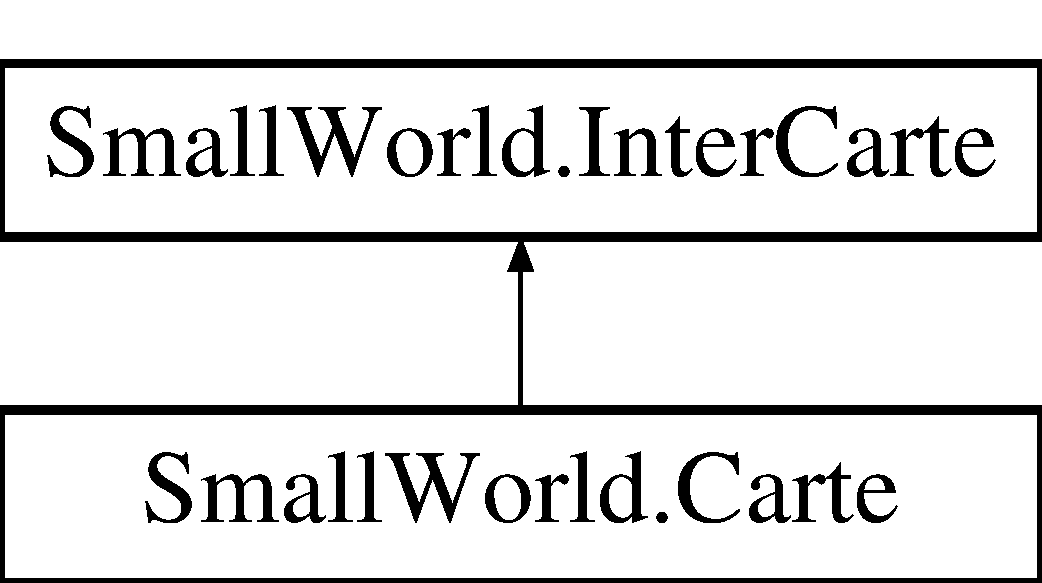
\includegraphics[height=2.000000cm]{class_small_world_1_1_carte}
\end{center}
\end{figure}
\subsection*{Public Member Functions}
\begin{DoxyCompactItemize}
\item 
\hyperlink{class_small_world_1_1_carte_add6995dddd2c8d509abf7a7cb8c4448d}{Carte} ()
\begin{DoxyCompactList}\small\item\em Constructeur d'une nouvelle \hyperlink{class_small_world_1_1_carte}{Carte} vide. \end{DoxyCompactList}\item 
\hyperlink{class_small_world_1_1_carte_a3795b7cf629c8e9151bbb2410bc39eb3}{Carte} (List$<$ List$<$ \hyperlink{class_small_world_1_1_case}{Case} $>$$>$ liste\-C)
\begin{DoxyCompactList}\small\item\em Constructeur d'une nouvelle \hyperlink{class_small_world_1_1_carte}{Carte}. \end{DoxyCompactList}\item 
void \hyperlink{class_small_world_1_1_carte_a412690bcb32264b5282913660c5e38f8}{creer\-Carte} ()
\begin{DoxyCompactList}\small\item\em Génération d'une nouvelle \hyperlink{class_small_world_1_1_carte}{Carte}. \end{DoxyCompactList}\item 
void \hyperlink{class_small_world_1_1_carte_aad692a68904925a11d5307181ca83c5f}{definir\-Strategie} (\hyperlink{class_small_world_1_1_strategie_carte}{Strategie\-Carte} strat)
\begin{DoxyCompactList}\small\item\em Définit la stratégie à adopter pour la génération d'une nouvelle carte. \end{DoxyCompactList}\end{DoxyCompactItemize}
\subsection*{Properties}
\begin{DoxyCompactItemize}
\item 
\hypertarget{class_small_world_1_1_carte_a8bb9a9efb0ee54e366886080b52db368}{int \hyperlink{class_small_world_1_1_carte_a8bb9a9efb0ee54e366886080b52db368}{Taille\-Carte}\hspace{0.3cm}{\ttfamily  \mbox{[}get, set\mbox{]}}}\label{class_small_world_1_1_carte_a8bb9a9efb0ee54e366886080b52db368}

\begin{DoxyCompactList}\small\item\em \hyperlink{namespace_small_world_1_1_properties}{Properties} pour l'attribut Taille\-Carte. \end{DoxyCompactList}\item 
\hypertarget{class_small_world_1_1_carte_a82f9d8a898502d6086db543456d01416}{\hyperlink{class_small_world_1_1_strategie_carte}{Strategie\-Carte} \hyperlink{class_small_world_1_1_carte_a82f9d8a898502d6086db543456d01416}{Strategie\-Carte}\hspace{0.3cm}{\ttfamily  \mbox{[}get, set\mbox{]}}}\label{class_small_world_1_1_carte_a82f9d8a898502d6086db543456d01416}

\begin{DoxyCompactList}\small\item\em \hyperlink{namespace_small_world_1_1_properties}{Properties} pour l'attribut strategie\-Carte. \end{DoxyCompactList}\item 
\hypertarget{class_small_world_1_1_carte_a829c1b8f4b2b6dbdb4c24b696ec7915e}{List$<$ List$<$ \hyperlink{class_small_world_1_1_case}{Case} $>$ $>$ \hyperlink{class_small_world_1_1_carte_a829c1b8f4b2b6dbdb4c24b696ec7915e}{Liste\-Cases}\hspace{0.3cm}{\ttfamily  \mbox{[}get, set\mbox{]}}}\label{class_small_world_1_1_carte_a829c1b8f4b2b6dbdb4c24b696ec7915e}

\begin{DoxyCompactList}\small\item\em \hyperlink{namespace_small_world_1_1_properties}{Properties} pour l'attribut liste\-Cases. \end{DoxyCompactList}\item 
\hypertarget{class_small_world_1_1_carte_aff7fdff10186056c40ef44c6472039f1}{\hyperlink{class_small_world_1_1_fabrique_case}{Fabrique\-Case} \hyperlink{class_small_world_1_1_carte_aff7fdff10186056c40ef44c6472039f1}{Fabrique\-Case}\hspace{0.3cm}{\ttfamily  \mbox{[}get, set\mbox{]}}}\label{class_small_world_1_1_carte_aff7fdff10186056c40ef44c6472039f1}

\begin{DoxyCompactList}\small\item\em \hyperlink{namespace_small_world_1_1_properties}{Properties} pour l'attribut fabrique\-Case. \end{DoxyCompactList}\end{DoxyCompactItemize}


\subsection{Detailed Description}
Classe \hyperlink{class_small_world_1_1_carte}{Carte} Représente la carte du monde. 

\subsection{Constructor \& Destructor Documentation}
\hypertarget{class_small_world_1_1_carte_add6995dddd2c8d509abf7a7cb8c4448d}{\index{Small\-World\-::\-Carte@{Small\-World\-::\-Carte}!Carte@{Carte}}
\index{Carte@{Carte}!SmallWorld::Carte@{Small\-World\-::\-Carte}}
\subsubsection[{Carte}]{\setlength{\rightskip}{0pt plus 5cm}Small\-World.\-Carte.\-Carte (
\begin{DoxyParamCaption}
{}
\end{DoxyParamCaption}
)}}\label{class_small_world_1_1_carte_add6995dddd2c8d509abf7a7cb8c4448d}


Constructeur d'une nouvelle \hyperlink{class_small_world_1_1_carte}{Carte} vide. 

\begin{DoxyReturn}{Returns}
La nouvelle \hyperlink{class_small_world_1_1_carte}{Carte} 
\end{DoxyReturn}
\hypertarget{class_small_world_1_1_carte_a3795b7cf629c8e9151bbb2410bc39eb3}{\index{Small\-World\-::\-Carte@{Small\-World\-::\-Carte}!Carte@{Carte}}
\index{Carte@{Carte}!SmallWorld::Carte@{Small\-World\-::\-Carte}}
\subsubsection[{Carte}]{\setlength{\rightskip}{0pt plus 5cm}Small\-World.\-Carte.\-Carte (
\begin{DoxyParamCaption}
\item[{List$<$ List$<$ {\bf Case} $>$$>$}]{liste\-C}
\end{DoxyParamCaption}
)}}\label{class_small_world_1_1_carte_a3795b7cf629c8e9151bbb2410bc39eb3}


Constructeur d'une nouvelle \hyperlink{class_small_world_1_1_carte}{Carte}. 

Construit une nouvelle \hyperlink{class_small_world_1_1_carte}{Carte} à l'aide d'une liste de Cases


\begin{DoxyParams}{Parameters}
{\em List$<$\-List$<$\-Case$>$$>$} & {\bfseries liste\-C} La liste des cases formant la carte \\
\hline
\end{DoxyParams}
\begin{DoxyReturn}{Returns}
La nouvelle \hyperlink{class_small_world_1_1_carte}{Carte} 
\end{DoxyReturn}


\subsection{Member Function Documentation}
\hypertarget{class_small_world_1_1_carte_a412690bcb32264b5282913660c5e38f8}{\index{Small\-World\-::\-Carte@{Small\-World\-::\-Carte}!creer\-Carte@{creer\-Carte}}
\index{creer\-Carte@{creer\-Carte}!SmallWorld::Carte@{Small\-World\-::\-Carte}}
\subsubsection[{creer\-Carte}]{\setlength{\rightskip}{0pt plus 5cm}Small\-World.\-Carte.\-creer\-Carte (
\begin{DoxyParamCaption}
{}
\end{DoxyParamCaption}
)}}\label{class_small_world_1_1_carte_a412690bcb32264b5282913660c5e38f8}


Génération d'une nouvelle \hyperlink{class_small_world_1_1_carte}{Carte}. 

Génère une nouvelle \hyperlink{class_small_world_1_1_carte}{Carte}, suivant la stratégie demandée

\begin{DoxyReturn}{Returns}
void 
\end{DoxyReturn}


Implements \hyperlink{interface_small_world_1_1_inter_carte_a825e1748eb1a8f93dfe8aecdfc661064}{Small\-World.\-Inter\-Carte}.

\hypertarget{class_small_world_1_1_carte_aad692a68904925a11d5307181ca83c5f}{\index{Small\-World\-::\-Carte@{Small\-World\-::\-Carte}!definir\-Strategie@{definir\-Strategie}}
\index{definir\-Strategie@{definir\-Strategie}!SmallWorld::Carte@{Small\-World\-::\-Carte}}
\subsubsection[{definir\-Strategie}]{\setlength{\rightskip}{0pt plus 5cm}Small\-World.\-Carte.\-definir\-Strategie (
\begin{DoxyParamCaption}
\item[{{\bf Strategie\-Carte}}]{strat}
\end{DoxyParamCaption}
)}}\label{class_small_world_1_1_carte_aad692a68904925a11d5307181ca83c5f}


Définit la stratégie à adopter pour la génération d'une nouvelle carte. 


\begin{DoxyParams}{Parameters}
{\em \hyperlink{class_small_world_1_1_strategie_carte}{Strategie\-Carte}} & {\bfseries strat} La nouvelle stratégie à adopter \\
\hline
\end{DoxyParams}
\begin{DoxyReturn}{Returns}
void 
\end{DoxyReturn}


Implements \hyperlink{interface_small_world_1_1_inter_carte_a23c669cb523f222f53e8ab91a8944472}{Small\-World.\-Inter\-Carte}.



The documentation for this class was generated from the following file\-:\begin{DoxyCompactItemize}
\item 
C\-:/\-Users/damienc/\-Documents/\-Git\-Hub/\-Small\-World/\-Visual\-Studio/\-Projet\-P\-O\-O/\hyperlink{_carte_8cs}{Carte.\-cs}\end{DoxyCompactItemize}

\hypertarget{class_small_world_1_1_case}{\section{Small\-World.\-Case Class Reference}
\label{class_small_world_1_1_case}\index{Small\-World.\-Case@{Small\-World.\-Case}}
}


classe abstraite \hyperlink{class_small_world_1_1_case}{Case}  


Inheritance diagram for Small\-World.\-Case\-:\begin{figure}[H]
\begin{center}
\leavevmode
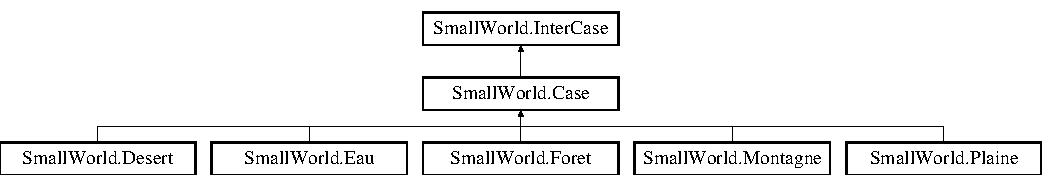
\includegraphics[height=2.349650cm]{class_small_world_1_1_case}
\end{center}
\end{figure}


\subsection{Detailed Description}
classe abstraite \hyperlink{class_small_world_1_1_case}{Case} 

The documentation for this class was generated from the following file\-:\begin{DoxyCompactItemize}
\item 
C\-:/\-Users/damienc/\-Documents/\-Git\-Hub/\-Small\-World/\-Visual\-Studio/\-Projet\-P\-O\-O/\hyperlink{_case_8cs}{Case.\-cs}\end{DoxyCompactItemize}

\hypertarget{class_small_world_1_1_constantes}{\section{Small\-World.\-Constantes Class Reference}
\label{class_small_world_1_1_constantes}\index{Small\-World.\-Constantes@{Small\-World.\-Constantes}}
}


Les différentes constantes du jeu \hyperlink{namespace_small_world}{Small\-World}.  


\subsection*{Public Attributes}
\begin{DoxyCompactItemize}
\item 
\hypertarget{class_small_world_1_1_constantes_a23455cae9ae5636a7b927748658f2bdf}{const int {\bfseries C\-A\-S\-E\-\_\-\-D\-E\-S\-E\-R\-T} = 0}\label{class_small_world_1_1_constantes_a23455cae9ae5636a7b927748658f2bdf}

\item 
\hypertarget{class_small_world_1_1_constantes_a9987d45381c9d786e7d57ac2e307661c}{const int {\bfseries C\-A\-S\-E\-\_\-\-E\-A\-U} = 1}\label{class_small_world_1_1_constantes_a9987d45381c9d786e7d57ac2e307661c}

\item 
\hypertarget{class_small_world_1_1_constantes_a6661fb0a373e616a7d8fe1217d59eeca}{const int {\bfseries C\-A\-S\-E\-\_\-\-F\-O\-R\-E\-T} = 2}\label{class_small_world_1_1_constantes_a6661fb0a373e616a7d8fe1217d59eeca}

\item 
\hypertarget{class_small_world_1_1_constantes_a720fc71ee09486e9a54c26a693472b73}{const int {\bfseries C\-A\-S\-E\-\_\-\-M\-O\-N\-T\-A\-G\-N\-E} = 3}\label{class_small_world_1_1_constantes_a720fc71ee09486e9a54c26a693472b73}

\item 
\hypertarget{class_small_world_1_1_constantes_a54cd0a73893539af192cb2e5964cab39}{const int {\bfseries C\-A\-S\-E\-\_\-\-P\-L\-A\-I\-N\-E} = 4}\label{class_small_world_1_1_constantes_a54cd0a73893539af192cb2e5964cab39}

\item 
\hypertarget{class_small_world_1_1_constantes_a53e6236fc2206e6016df7d3b54dee83e}{const string {\bfseries P\-E\-U\-P\-L\-E\-\_\-\-G\-A\-U\-L\-O\-I\-S} = \char`\"{}Gaulois\char`\"{}}\label{class_small_world_1_1_constantes_a53e6236fc2206e6016df7d3b54dee83e}

\item 
\hypertarget{class_small_world_1_1_constantes_ae68a2b6675d0fd610250e4272fd53a19}{const string {\bfseries P\-E\-U\-P\-L\-E\-\_\-\-N\-A\-I\-N} = \char`\"{}Nains\char`\"{}}\label{class_small_world_1_1_constantes_ae68a2b6675d0fd610250e4272fd53a19}

\item 
\hypertarget{class_small_world_1_1_constantes_a6c3dd4a547a47b023eef754d03bffb3e}{const string {\bfseries P\-E\-U\-P\-L\-E\-\_\-\-V\-I\-K\-I\-N\-G} = \char`\"{}Vikings\char`\"{}}\label{class_small_world_1_1_constantes_a6c3dd4a547a47b023eef754d03bffb3e}

\item 
\hypertarget{class_small_world_1_1_constantes_a6f0a0b7066f95a4b71705fbb6c2de7b4}{const string {\bfseries C\-A\-R\-T\-E\-\_\-\-D\-E\-M\-O} = \char`\"{}Démo\char`\"{}}\label{class_small_world_1_1_constantes_a6f0a0b7066f95a4b71705fbb6c2de7b4}

\item 
\hypertarget{class_small_world_1_1_constantes_a00b018aad32fc763782bc4d0e9dae049}{const string {\bfseries C\-A\-R\-T\-E\-\_\-\-P\-E\-T\-I\-T\-E} = \char`\"{}Petite\char`\"{}}\label{class_small_world_1_1_constantes_a00b018aad32fc763782bc4d0e9dae049}

\item 
\hypertarget{class_small_world_1_1_constantes_a1b50610f0a1f1a9100ab2ab5eba2cd41}{const string {\bfseries C\-A\-R\-T\-E\-\_\-\-N\-O\-R\-M\-A\-L\-E} = \char`\"{}Normale\char`\"{}}\label{class_small_world_1_1_constantes_a1b50610f0a1f1a9100ab2ab5eba2cd41}

\item 
\hypertarget{class_small_world_1_1_constantes_a4cc08f06c9ba0fb0ee650f77d3c0b7ac}{const int {\bfseries N\-B\-\_\-\-U\-N\-I\-T\-E\-\_\-\-D\-E\-M\-O} = 4}\label{class_small_world_1_1_constantes_a4cc08f06c9ba0fb0ee650f77d3c0b7ac}

\item 
\hypertarget{class_small_world_1_1_constantes_a2591cf46fa8dd2d0512227795c64fdc0}{const int {\bfseries N\-B\-\_\-\-U\-N\-I\-T\-E\-\_\-\-P\-E\-T\-I\-T\-E} = 6}\label{class_small_world_1_1_constantes_a2591cf46fa8dd2d0512227795c64fdc0}

\item 
\hypertarget{class_small_world_1_1_constantes_a71bcce9b2d03223425ae08a022c55a68}{const int {\bfseries N\-B\-\_\-\-U\-N\-I\-T\-E\-\_\-\-N\-O\-R\-M\-A\-L\-E} = 8}\label{class_small_world_1_1_constantes_a71bcce9b2d03223425ae08a022c55a68}

\item 
\hypertarget{class_small_world_1_1_constantes_ae5e9ff23cff7ddfb3735e7b2bf83dd0f}{const int {\bfseries N\-B\-\_\-\-T\-O\-U\-R\-\_\-\-D\-E\-M\-O} = 5}\label{class_small_world_1_1_constantes_ae5e9ff23cff7ddfb3735e7b2bf83dd0f}

\item 
\hypertarget{class_small_world_1_1_constantes_a0540886588eca12e8e8eae08c9229c39}{const int {\bfseries N\-B\-\_\-\-T\-O\-U\-R\-\_\-\-P\-E\-T\-I\-T\-E} = 20}\label{class_small_world_1_1_constantes_a0540886588eca12e8e8eae08c9229c39}

\item 
\hypertarget{class_small_world_1_1_constantes_a55fe56d58859a77f0d2bece1e29a8232}{const int {\bfseries N\-B\-\_\-\-T\-O\-U\-R\-\_\-\-N\-O\-R\-M\-A\-L\-E} = 30}\label{class_small_world_1_1_constantes_a55fe56d58859a77f0d2bece1e29a8232}

\item 
\hypertarget{class_small_world_1_1_constantes_a8d4790413b87e8a595eac28799dbc3b6}{const int {\bfseries N\-B\-\_\-\-C\-A\-S\-E\-\_\-\-D\-E\-M\-O} = 5}\label{class_small_world_1_1_constantes_a8d4790413b87e8a595eac28799dbc3b6}

\item 
\hypertarget{class_small_world_1_1_constantes_a8b0403aadf23e4c72d40641429dd0f32}{const int {\bfseries N\-B\-\_\-\-C\-A\-S\-E\-\_\-\-P\-E\-T\-I\-T\-E} = 10}\label{class_small_world_1_1_constantes_a8b0403aadf23e4c72d40641429dd0f32}

\item 
\hypertarget{class_small_world_1_1_constantes_abc2fdb8eedc292e10c0c544a08cf5f7e}{const int {\bfseries N\-B\-\_\-\-C\-A\-S\-E\-\_\-\-N\-O\-R\-M\-A\-L\-E} = 15}\label{class_small_world_1_1_constantes_abc2fdb8eedc292e10c0c544a08cf5f7e}

\item 
\hypertarget{class_small_world_1_1_constantes_a989e7595d2fa73e0c2ad8f60da381dfc}{const int {\bfseries P\-O\-I\-N\-T\-\_\-\-C\-A\-S\-E} = 1}\label{class_small_world_1_1_constantes_a989e7595d2fa73e0c2ad8f60da381dfc}

\item 
\hypertarget{class_small_world_1_1_constantes_aaf9551b229c72e6284ae4d190374d9b2}{const int {\bfseries U\-N\-I\-T\-E\-\_\-\-P\-O\-I\-N\-T\-\_\-\-D\-E\-P\-L} = 2}\label{class_small_world_1_1_constantes_aaf9551b229c72e6284ae4d190374d9b2}

\item 
\hypertarget{class_small_world_1_1_constantes_a6671bb3e6cfbeddc54c81dfacc9d242f}{const int {\bfseries U\-N\-I\-T\-E\-\_\-\-P\-O\-I\-N\-T\-\_\-\-A\-T\-T} = 2}\label{class_small_world_1_1_constantes_a6671bb3e6cfbeddc54c81dfacc9d242f}

\item 
\hypertarget{class_small_world_1_1_constantes_af35965bfcbd7b7772fd3e4284605cc11}{const int {\bfseries U\-N\-I\-T\-E\-\_\-\-P\-O\-I\-N\-T\-\_\-\-D\-E\-F} = 1}\label{class_small_world_1_1_constantes_af35965bfcbd7b7772fd3e4284605cc11}

\item 
\hypertarget{class_small_world_1_1_constantes_ab6c527d71bef08dfa0589b918c8394b5}{const int {\bfseries U\-N\-I\-T\-E\-\_\-\-P\-O\-I\-N\-T\-\_\-\-V\-I\-E} = 5}\label{class_small_world_1_1_constantes_ab6c527d71bef08dfa0589b918c8394b5}

\end{DoxyCompactItemize}


\subsection{Detailed Description}
Les différentes constantes du jeu \hyperlink{namespace_small_world}{Small\-World}. 

The documentation for this class was generated from the following file\-:\begin{DoxyCompactItemize}
\item 
C\-:/\-Users/damienc/\-Documents/\-Git\-Hub/\-Small\-World/\-Visual\-Studio/\-Projet\-P\-O\-O/\hyperlink{_constantes_8cs}{Constantes.\-cs}\end{DoxyCompactItemize}

\hypertarget{class_small_world_1_1_coordonnees}{\section{Small\-World.\-Coordonnees Class Reference}
\label{class_small_world_1_1_coordonnees}\index{Small\-World.\-Coordonnees@{Small\-World.\-Coordonnees}}
}


Rprésentation des coordonnées.  


Inheritance diagram for Small\-World.\-Coordonnees\-:\begin{figure}[H]
\begin{center}
\leavevmode
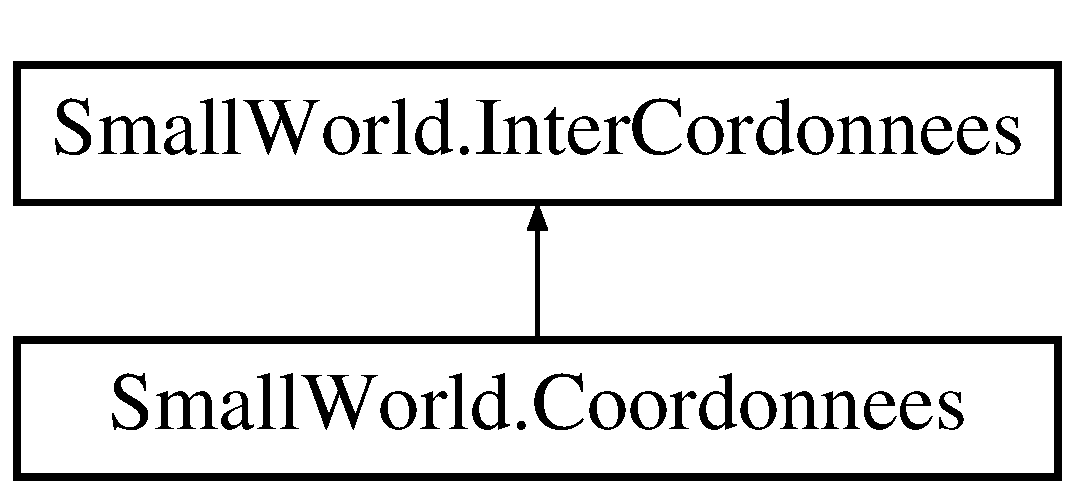
\includegraphics[height=2.000000cm]{class_small_world_1_1_coordonnees}
\end{center}
\end{figure}
\subsection*{Public Member Functions}
\begin{DoxyCompactItemize}
\item 
\hyperlink{class_small_world_1_1_coordonnees_aec13aa49810f6cb62c6b73c04fa9ebbe}{Coordonnees} (int abs, int ord)
\begin{DoxyCompactList}\small\item\em Constructeur de coordonnees. \end{DoxyCompactList}\item 
\hyperlink{class_small_world_1_1_coordonnees_a3e91ea13cf001b39eb63ca45345fd058}{Coordonnees} ()
\begin{DoxyCompactList}\small\item\em Constructeur de coordonnees. \end{DoxyCompactList}\item 
override bool \hyperlink{class_small_world_1_1_coordonnees_aa5bcb46ee14473b4a7c62442f7290ce1}{Equals} (Object obj)
\begin{DoxyCompactList}\small\item\em Test d'égalité pour deux coordonnées. \end{DoxyCompactList}\item 
override int \hyperlink{class_small_world_1_1_coordonnees_a8e05913286d547f5261480d8f03c5453}{Get\-Hash\-Code} ()
\begin{DoxyCompactList}\small\item\em return la clef de hash de l'objet \end{DoxyCompactList}\end{DoxyCompactItemize}
\subsection*{Properties}
\begin{DoxyCompactItemize}
\item 
\hypertarget{class_small_world_1_1_coordonnees_a08f32128a4ff9c97430d4ae8075c444a}{int \hyperlink{class_small_world_1_1_coordonnees_a08f32128a4ff9c97430d4ae8075c444a}{Abscisse}\hspace{0.3cm}{\ttfamily  \mbox{[}get, set\mbox{]}}}\label{class_small_world_1_1_coordonnees_a08f32128a4ff9c97430d4ae8075c444a}

\begin{DoxyCompactList}\small\item\em \hyperlink{namespace_small_world_1_1_properties}{Properties} pour l'attribut abscisse. \end{DoxyCompactList}\item 
\hypertarget{class_small_world_1_1_coordonnees_aac7114725ff9eaa08f7cc8588a13ed49}{int \hyperlink{class_small_world_1_1_coordonnees_aac7114725ff9eaa08f7cc8588a13ed49}{Ordonnee}\hspace{0.3cm}{\ttfamily  \mbox{[}get, set\mbox{]}}}\label{class_small_world_1_1_coordonnees_aac7114725ff9eaa08f7cc8588a13ed49}

\begin{DoxyCompactList}\small\item\em \hyperlink{namespace_small_world_1_1_properties}{Properties} pour l'attribut ordonnee. \end{DoxyCompactList}\end{DoxyCompactItemize}


\subsection{Detailed Description}
Rprésentation des coordonnées. 

\subsection{Constructor \& Destructor Documentation}
\hypertarget{class_small_world_1_1_coordonnees_aec13aa49810f6cb62c6b73c04fa9ebbe}{\index{Small\-World\-::\-Coordonnees@{Small\-World\-::\-Coordonnees}!Coordonnees@{Coordonnees}}
\index{Coordonnees@{Coordonnees}!SmallWorld::Coordonnees@{Small\-World\-::\-Coordonnees}}
\subsubsection[{Coordonnees}]{\setlength{\rightskip}{0pt plus 5cm}Small\-World.\-Coordonnees.\-Coordonnees (
\begin{DoxyParamCaption}
\item[{int}]{abs, }
\item[{int}]{ord}
\end{DoxyParamCaption}
)}}\label{class_small_world_1_1_coordonnees_aec13aa49810f6cb62c6b73c04fa9ebbe}


Constructeur de coordonnees. 


\begin{DoxyParams}{Parameters}
{\em int} & {\bfseries abs} L'abscisse \\
\hline
{\em int} & {\bfseries ord} L'ordonnée \\
\hline
\end{DoxyParams}
\begin{DoxyReturn}{Returns}
les nouvelles coordonnées 
\end{DoxyReturn}
\hypertarget{class_small_world_1_1_coordonnees_a3e91ea13cf001b39eb63ca45345fd058}{\index{Small\-World\-::\-Coordonnees@{Small\-World\-::\-Coordonnees}!Coordonnees@{Coordonnees}}
\index{Coordonnees@{Coordonnees}!SmallWorld::Coordonnees@{Small\-World\-::\-Coordonnees}}
\subsubsection[{Coordonnees}]{\setlength{\rightskip}{0pt plus 5cm}Small\-World.\-Coordonnees.\-Coordonnees (
\begin{DoxyParamCaption}
{}
\end{DoxyParamCaption}
)}}\label{class_small_world_1_1_coordonnees_a3e91ea13cf001b39eb63ca45345fd058}


Constructeur de coordonnees. 

\begin{DoxyReturn}{Returns}
les nouvelles coordonnées 
\end{DoxyReturn}


\subsection{Member Function Documentation}
\hypertarget{class_small_world_1_1_coordonnees_aa5bcb46ee14473b4a7c62442f7290ce1}{\index{Small\-World\-::\-Coordonnees@{Small\-World\-::\-Coordonnees}!Equals@{Equals}}
\index{Equals@{Equals}!SmallWorld::Coordonnees@{Small\-World\-::\-Coordonnees}}
\subsubsection[{Equals}]{\setlength{\rightskip}{0pt plus 5cm}Small\-World.\-Coordonnees.\-Equals (
\begin{DoxyParamCaption}
\item[{Object}]{obj}
\end{DoxyParamCaption}
)}}\label{class_small_world_1_1_coordonnees_aa5bcb46ee14473b4a7c62442f7290ce1}


Test d'égalité pour deux coordonnées. 


\begin{DoxyParams}{Parameters}
{\em Object} & {\bfseries obj} la coordonnée à comparer \\
\hline
\end{DoxyParams}
\begin{DoxyReturn}{Returns}
bool vrai si les deux coordonnées sont égales, faux sinon 
\end{DoxyReturn}
\hypertarget{class_small_world_1_1_coordonnees_a8e05913286d547f5261480d8f03c5453}{\index{Small\-World\-::\-Coordonnees@{Small\-World\-::\-Coordonnees}!Get\-Hash\-Code@{Get\-Hash\-Code}}
\index{Get\-Hash\-Code@{Get\-Hash\-Code}!SmallWorld::Coordonnees@{Small\-World\-::\-Coordonnees}}
\subsubsection[{Get\-Hash\-Code}]{\setlength{\rightskip}{0pt plus 5cm}Small\-World.\-Coordonnees.\-Get\-Hash\-Code (
\begin{DoxyParamCaption}
{}
\end{DoxyParamCaption}
)}}\label{class_small_world_1_1_coordonnees_a8e05913286d547f5261480d8f03c5453}


return la clef de hash de l'objet 

\begin{DoxyReturn}{Returns}
int la clef de hash 
\end{DoxyReturn}


The documentation for this class was generated from the following file\-:\begin{DoxyCompactItemize}
\item 
C\-:/\-Users/damienc/\-Documents/\-Git\-Hub/\-Small\-World/\-Visual\-Studio/\-Projet\-P\-O\-O/\hyperlink{_coordonnees_8cs}{Coordonnees.\-cs}\end{DoxyCompactItemize}

\hypertarget{class_small_world_1_1_createur_partie}{\section{Small\-World.\-Createur\-Partie Class Reference}
\label{class_small_world_1_1_createur_partie}\index{Small\-World.\-Createur\-Partie@{Small\-World.\-Createur\-Partie}}
}


Classe du créateur de partie.  


Inheritance diagram for Small\-World.\-Createur\-Partie\-:\begin{figure}[H]
\begin{center}
\leavevmode
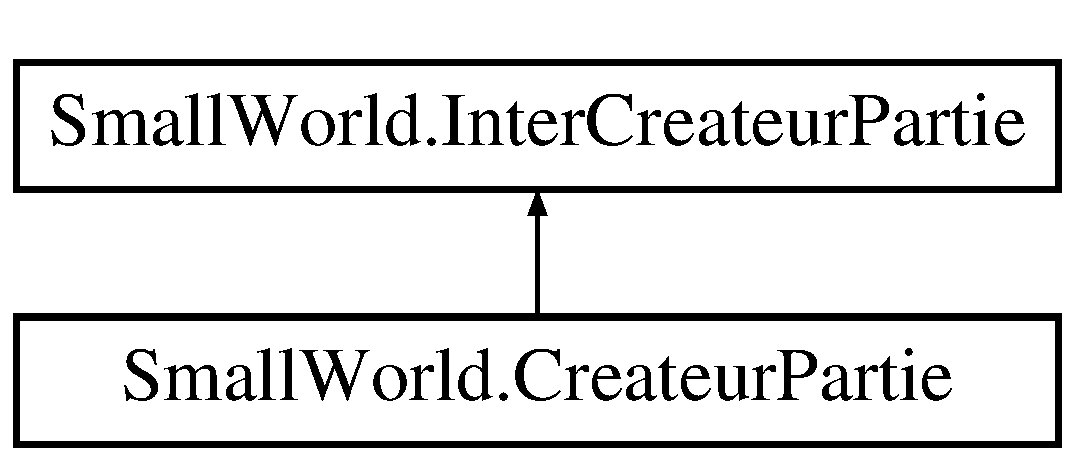
\includegraphics[height=2.000000cm]{class_small_world_1_1_createur_partie}
\end{center}
\end{figure}
\subsection*{Public Member Functions}
\begin{DoxyCompactItemize}
\item 
\hyperlink{class_small_world_1_1_createur_partie_a6b32ea8a3b1daeb8530dd882b3791838}{Createur\-Partie} ()
\begin{DoxyCompactList}\small\item\em Constructeur du créateur de partie. \end{DoxyCompactList}\item 
void \hyperlink{class_small_world_1_1_createur_partie_a1388144440304d2d82879a15e0e58e1f}{ajout\-Joueur} (string nom, string peuple)
\begin{DoxyCompactList}\small\item\em Ajouter un joueur à la partie. \end{DoxyCompactList}\item 
\hyperlink{class_small_world_1_1_partie}{Partie} \hyperlink{class_small_world_1_1_createur_partie_a434764cadcd4b11f8b171ed8becfdc6d}{construire} ()
\begin{DoxyCompactList}\small\item\em Construction d'une nouvelle partie. \end{DoxyCompactList}\end{DoxyCompactItemize}
\subsection*{Properties}
\begin{DoxyCompactItemize}
\item 
\hypertarget{class_small_world_1_1_createur_partie_a8046b4b5283f857d49038aa5f83a5613}{\hyperlink{class_small_world_1_1_monteur_partie}{Monteur\-Partie} \hyperlink{class_small_world_1_1_createur_partie_a8046b4b5283f857d49038aa5f83a5613}{Monteur\-Partie}\hspace{0.3cm}{\ttfamily  \mbox{[}get, set\mbox{]}}}\label{class_small_world_1_1_createur_partie_a8046b4b5283f857d49038aa5f83a5613}

\begin{DoxyCompactList}\small\item\em \hyperlink{namespace_small_world_1_1_properties}{Properties} pour l'attribut \hyperlink{class_small_world_1_1_monteur_partie}{Monteur\-Partie}. \end{DoxyCompactList}\item 
\hypertarget{class_small_world_1_1_createur_partie_a4c4b3643c25110388e77e3a5ab18c50b}{string \hyperlink{class_small_world_1_1_createur_partie_a4c4b3643c25110388e77e3a5ab18c50b}{Type\-Partie}\hspace{0.3cm}{\ttfamily  \mbox{[}get, set\mbox{]}}}\label{class_small_world_1_1_createur_partie_a4c4b3643c25110388e77e3a5ab18c50b}

\begin{DoxyCompactList}\small\item\em \hyperlink{namespace_small_world_1_1_properties}{Properties} pour l'attribut type\-Partie. \end{DoxyCompactList}\end{DoxyCompactItemize}


\subsection{Detailed Description}
Classe du créateur de partie. 

\subsection{Constructor \& Destructor Documentation}
\hypertarget{class_small_world_1_1_createur_partie_a6b32ea8a3b1daeb8530dd882b3791838}{\index{Small\-World\-::\-Createur\-Partie@{Small\-World\-::\-Createur\-Partie}!Createur\-Partie@{Createur\-Partie}}
\index{Createur\-Partie@{Createur\-Partie}!SmallWorld::CreateurPartie@{Small\-World\-::\-Createur\-Partie}}
\subsubsection[{Createur\-Partie}]{\setlength{\rightskip}{0pt plus 5cm}Small\-World.\-Createur\-Partie.\-Createur\-Partie (
\begin{DoxyParamCaption}
{}
\end{DoxyParamCaption}
)}}\label{class_small_world_1_1_createur_partie_a6b32ea8a3b1daeb8530dd882b3791838}


Constructeur du créateur de partie. 

\begin{DoxyReturn}{Returns}
\hyperlink{class_small_world_1_1_createur_partie}{Createur\-Partie} 
\end{DoxyReturn}


\subsection{Member Function Documentation}
\hypertarget{class_small_world_1_1_createur_partie_a1388144440304d2d82879a15e0e58e1f}{\index{Small\-World\-::\-Createur\-Partie@{Small\-World\-::\-Createur\-Partie}!ajout\-Joueur@{ajout\-Joueur}}
\index{ajout\-Joueur@{ajout\-Joueur}!SmallWorld::CreateurPartie@{Small\-World\-::\-Createur\-Partie}}
\subsubsection[{ajout\-Joueur}]{\setlength{\rightskip}{0pt plus 5cm}Small\-World.\-Createur\-Partie.\-ajout\-Joueur (
\begin{DoxyParamCaption}
\item[{string}]{nom, }
\item[{string}]{peuple}
\end{DoxyParamCaption}
)}}\label{class_small_world_1_1_createur_partie_a1388144440304d2d82879a15e0e58e1f}


Ajouter un joueur à la partie. 


\begin{DoxyParams}{Parameters}
{\em string} & {\bfseries nom} le nom du joueur \\
\hline
{\em string} & {\bfseries peuple} le type de peuple \\
\hline
\end{DoxyParams}
\begin{DoxyReturn}{Returns}
void 
\end{DoxyReturn}


Implements \hyperlink{interface_small_world_1_1_inter_createur_partie_af3fa5aaff01c6709b99eff93b6252da5}{Small\-World.\-Inter\-Createur\-Partie}.

\hypertarget{class_small_world_1_1_createur_partie_a434764cadcd4b11f8b171ed8becfdc6d}{\index{Small\-World\-::\-Createur\-Partie@{Small\-World\-::\-Createur\-Partie}!construire@{construire}}
\index{construire@{construire}!SmallWorld::CreateurPartie@{Small\-World\-::\-Createur\-Partie}}
\subsubsection[{construire}]{\setlength{\rightskip}{0pt plus 5cm}Small\-World.\-Createur\-Partie.\-construire (
\begin{DoxyParamCaption}
{}
\end{DoxyParamCaption}
)}}\label{class_small_world_1_1_createur_partie_a434764cadcd4b11f8b171ed8becfdc6d}


Construction d'une nouvelle partie. 

\begin{DoxyReturn}{Returns}
void 
\end{DoxyReturn}


Implements \hyperlink{interface_small_world_1_1_inter_createur_partie_a84bc048d2a71699fef54ef531477c917}{Small\-World.\-Inter\-Createur\-Partie}.



The documentation for this class was generated from the following file\-:\begin{DoxyCompactItemize}
\item 
C\-:/\-Users/damienc/\-Documents/\-Git\-Hub/\-Small\-World/\-Visual\-Studio/\-Projet\-P\-O\-O/\hyperlink{_createur_partie_8cs}{Createur\-Partie.\-cs}\end{DoxyCompactItemize}

\hypertarget{class_small_world_1_1_desert}{\section{Small\-World.\-Desert Class Reference}
\label{class_small_world_1_1_desert}\index{Small\-World.\-Desert@{Small\-World.\-Desert}}
}
Inheritance diagram for Small\-World.\-Desert\-:\begin{figure}[H]
\begin{center}
\leavevmode
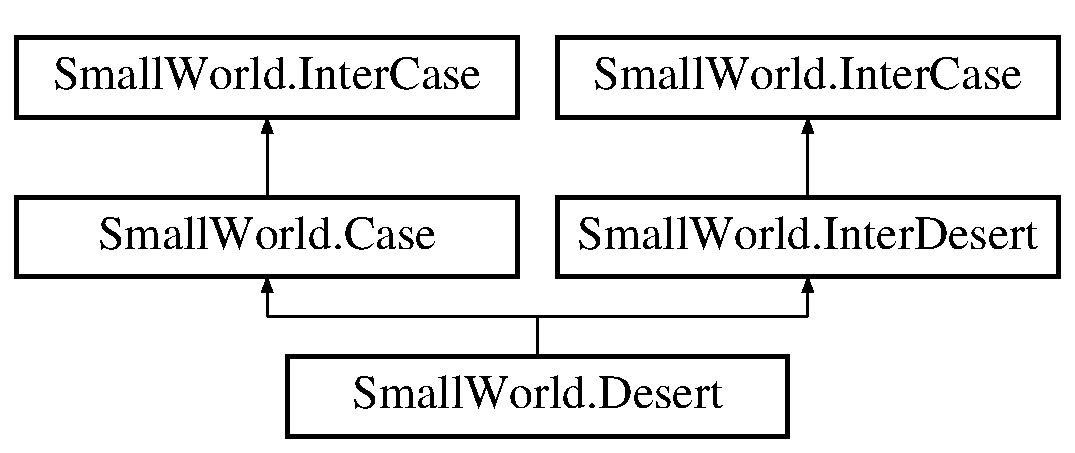
\includegraphics[height=3.000000cm]{class_small_world_1_1_desert}
\end{center}
\end{figure}


The documentation for this class was generated from the following file\-:\begin{DoxyCompactItemize}
\item 
C\-:/\-Users/damienc/\-Documents/\-Git\-Hub/\-Small\-World/\-Visual\-Studio/\-Projet\-P\-O\-O/desert.\-cs\end{DoxyCompactItemize}

\hypertarget{class_small_world_1_1_eau}{\section{Small\-World.\-Eau Class Reference}
\label{class_small_world_1_1_eau}\index{Small\-World.\-Eau@{Small\-World.\-Eau}}
}


class pour \hyperlink{class_small_world_1_1_case}{Case} de type eau  


Inheritance diagram for Small\-World.\-Eau\-:\begin{figure}[H]
\begin{center}
\leavevmode
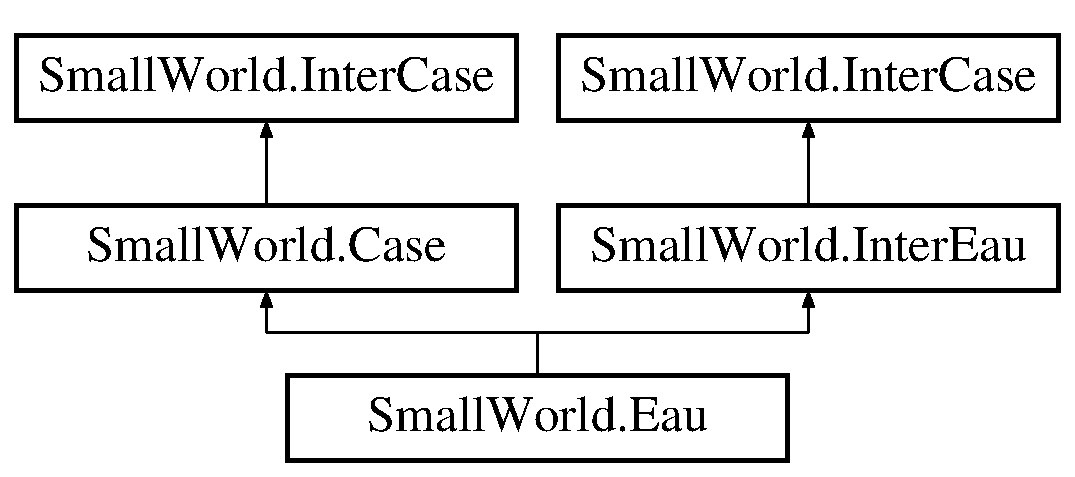
\includegraphics[height=3.000000cm]{class_small_world_1_1_eau}
\end{center}
\end{figure}


\subsection{Detailed Description}
class pour \hyperlink{class_small_world_1_1_case}{Case} de type eau 

The documentation for this class was generated from the following file\-:\begin{DoxyCompactItemize}
\item 
C\-:/\-Users/damienc/\-Documents/\-Git\-Hub/\-Small\-World/\-Visual\-Studio/\-Projet\-P\-O\-O/\hyperlink{_case_8cs}{Case.\-cs}\end{DoxyCompactItemize}

\hypertarget{class_small_world_1_1_fabrique_case}{\section{Small\-World.\-Fabrique\-Case Class Reference}
\label{class_small_world_1_1_fabrique_case}\index{Small\-World.\-Fabrique\-Case@{Small\-World.\-Fabrique\-Case}}
}


classe \hyperlink{class_small_world_1_1_fabrique_case}{Fabrique\-Case} pour la génération de cases  


Inheritance diagram for Small\-World.\-Fabrique\-Case\-:\begin{figure}[H]
\begin{center}
\leavevmode
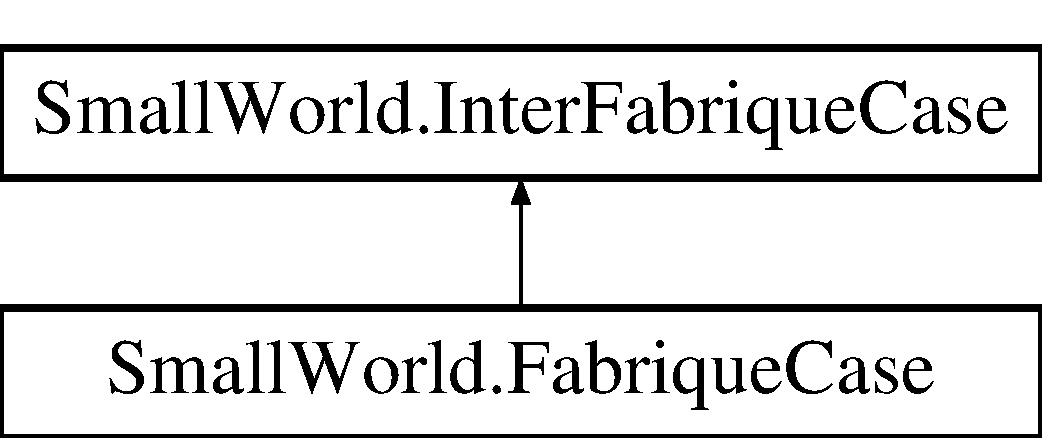
\includegraphics[height=2.000000cm]{class_small_world_1_1_fabrique_case}
\end{center}
\end{figure}
\subsection*{Public Member Functions}
\begin{DoxyCompactItemize}
\item 
\hyperlink{class_small_world_1_1_case}{Case} \hyperlink{class_small_world_1_1_fabrique_case_add84ef5fe1dda0653f391ce3d174f1cf}{obtenir\-Desert} ()
\begin{DoxyCompactList}\small\item\em Obtenir une case de type \hyperlink{class_small_world_1_1_desert}{Desert}. \end{DoxyCompactList}\item 
\hyperlink{class_small_world_1_1_case}{Case} \hyperlink{class_small_world_1_1_fabrique_case_a1da8866890280c611893961e85ffddbb}{obtenir\-Eau} ()
\begin{DoxyCompactList}\small\item\em Obtenir une case de type \hyperlink{class_small_world_1_1_eau}{Eau}. \end{DoxyCompactList}\item 
\hyperlink{class_small_world_1_1_case}{Case} \hyperlink{class_small_world_1_1_fabrique_case_a391674c9165245c355aaa043028d5027}{obtenir\-Foret} ()
\begin{DoxyCompactList}\small\item\em Obtenir une case de type \hyperlink{class_small_world_1_1_foret}{Foret}. \end{DoxyCompactList}\item 
\hyperlink{class_small_world_1_1_case}{Case} \hyperlink{class_small_world_1_1_fabrique_case_a4d50e880c85785212a7317a1d3fa4da6}{obtenir\-Montagne} ()
\begin{DoxyCompactList}\small\item\em Obtenir une case de type \hyperlink{class_small_world_1_1_montagne}{Montagne}. \end{DoxyCompactList}\item 
\hyperlink{class_small_world_1_1_case}{Case} \hyperlink{class_small_world_1_1_fabrique_case_ac80166926c7b4ed6761fcbb57688736e}{obtenir\-Plaine} ()
\begin{DoxyCompactList}\small\item\em Obtenir une case de type \hyperlink{class_small_world_1_1_plaine}{Plaine}. \end{DoxyCompactList}\end{DoxyCompactItemize}
\subsection*{Properties}
\begin{DoxyCompactItemize}
\item 
\hypertarget{class_small_world_1_1_fabrique_case_aede9c2f05ad6f6568af7ee8752b62438}{static \hyperlink{class_small_world_1_1_fabrique_case}{Fabrique\-Case} \hyperlink{class_small_world_1_1_fabrique_case_aede9c2f05ad6f6568af7ee8752b62438}{Instance\-\_\-\-Fab\-Case}\hspace{0.3cm}{\ttfamily  \mbox{[}get\mbox{]}}}\label{class_small_world_1_1_fabrique_case_aede9c2f05ad6f6568af7ee8752b62438}

\begin{DoxyCompactList}\small\item\em \hyperlink{namespace_small_world_1_1_properties}{Properties} pour l'attribut instance\-\_\-\-Fab\-Case. \end{DoxyCompactList}\end{DoxyCompactItemize}


\subsection{Detailed Description}
classe \hyperlink{class_small_world_1_1_fabrique_case}{Fabrique\-Case} pour la génération de cases 

\subsection{Member Function Documentation}
\hypertarget{class_small_world_1_1_fabrique_case_add84ef5fe1dda0653f391ce3d174f1cf}{\index{Small\-World\-::\-Fabrique\-Case@{Small\-World\-::\-Fabrique\-Case}!obtenir\-Desert@{obtenir\-Desert}}
\index{obtenir\-Desert@{obtenir\-Desert}!SmallWorld::FabriqueCase@{Small\-World\-::\-Fabrique\-Case}}
\subsubsection[{obtenir\-Desert}]{\setlength{\rightskip}{0pt plus 5cm}Small\-World.\-Fabrique\-Case.\-obtenir\-Desert (
\begin{DoxyParamCaption}
{}
\end{DoxyParamCaption}
)}}\label{class_small_world_1_1_fabrique_case_add84ef5fe1dda0653f391ce3d174f1cf}


Obtenir une case de type \hyperlink{class_small_world_1_1_desert}{Desert}. 

\begin{DoxyReturn}{Returns}
\hyperlink{class_small_world_1_1_case}{Case} une case \hyperlink{class_small_world_1_1_desert}{Desert} 
\end{DoxyReturn}


Implements \hyperlink{interface_small_world_1_1_inter_fabrique_case_ac376254f1e6e55abb83f079fc8793034}{Small\-World.\-Inter\-Fabrique\-Case}.

\hypertarget{class_small_world_1_1_fabrique_case_a1da8866890280c611893961e85ffddbb}{\index{Small\-World\-::\-Fabrique\-Case@{Small\-World\-::\-Fabrique\-Case}!obtenir\-Eau@{obtenir\-Eau}}
\index{obtenir\-Eau@{obtenir\-Eau}!SmallWorld::FabriqueCase@{Small\-World\-::\-Fabrique\-Case}}
\subsubsection[{obtenir\-Eau}]{\setlength{\rightskip}{0pt plus 5cm}Small\-World.\-Fabrique\-Case.\-obtenir\-Eau (
\begin{DoxyParamCaption}
{}
\end{DoxyParamCaption}
)}}\label{class_small_world_1_1_fabrique_case_a1da8866890280c611893961e85ffddbb}


Obtenir une case de type \hyperlink{class_small_world_1_1_eau}{Eau}. 

\begin{DoxyReturn}{Returns}
\hyperlink{class_small_world_1_1_case}{Case} une case \hyperlink{class_small_world_1_1_eau}{Eau} 
\end{DoxyReturn}


Implements \hyperlink{interface_small_world_1_1_inter_fabrique_case_a9dfab92cb279671297513e32d11994c1}{Small\-World.\-Inter\-Fabrique\-Case}.

\hypertarget{class_small_world_1_1_fabrique_case_a391674c9165245c355aaa043028d5027}{\index{Small\-World\-::\-Fabrique\-Case@{Small\-World\-::\-Fabrique\-Case}!obtenir\-Foret@{obtenir\-Foret}}
\index{obtenir\-Foret@{obtenir\-Foret}!SmallWorld::FabriqueCase@{Small\-World\-::\-Fabrique\-Case}}
\subsubsection[{obtenir\-Foret}]{\setlength{\rightskip}{0pt plus 5cm}Small\-World.\-Fabrique\-Case.\-obtenir\-Foret (
\begin{DoxyParamCaption}
{}
\end{DoxyParamCaption}
)}}\label{class_small_world_1_1_fabrique_case_a391674c9165245c355aaa043028d5027}


Obtenir une case de type \hyperlink{class_small_world_1_1_foret}{Foret}. 

\begin{DoxyReturn}{Returns}
\hyperlink{class_small_world_1_1_case}{Case} une case \hyperlink{class_small_world_1_1_foret}{Foret} 
\end{DoxyReturn}


Implements \hyperlink{interface_small_world_1_1_inter_fabrique_case_ac30d13640a58338ff314f3a289da5b8b}{Small\-World.\-Inter\-Fabrique\-Case}.

\hypertarget{class_small_world_1_1_fabrique_case_a4d50e880c85785212a7317a1d3fa4da6}{\index{Small\-World\-::\-Fabrique\-Case@{Small\-World\-::\-Fabrique\-Case}!obtenir\-Montagne@{obtenir\-Montagne}}
\index{obtenir\-Montagne@{obtenir\-Montagne}!SmallWorld::FabriqueCase@{Small\-World\-::\-Fabrique\-Case}}
\subsubsection[{obtenir\-Montagne}]{\setlength{\rightskip}{0pt plus 5cm}Small\-World.\-Fabrique\-Case.\-obtenir\-Montagne (
\begin{DoxyParamCaption}
{}
\end{DoxyParamCaption}
)}}\label{class_small_world_1_1_fabrique_case_a4d50e880c85785212a7317a1d3fa4da6}


Obtenir une case de type \hyperlink{class_small_world_1_1_montagne}{Montagne}. 

\begin{DoxyReturn}{Returns}
\hyperlink{class_small_world_1_1_case}{Case} une case \hyperlink{class_small_world_1_1_montagne}{Montagne} 
\end{DoxyReturn}


Implements \hyperlink{interface_small_world_1_1_inter_fabrique_case_a9d324c968a0926fe31f29199948dd9df}{Small\-World.\-Inter\-Fabrique\-Case}.

\hypertarget{class_small_world_1_1_fabrique_case_ac80166926c7b4ed6761fcbb57688736e}{\index{Small\-World\-::\-Fabrique\-Case@{Small\-World\-::\-Fabrique\-Case}!obtenir\-Plaine@{obtenir\-Plaine}}
\index{obtenir\-Plaine@{obtenir\-Plaine}!SmallWorld::FabriqueCase@{Small\-World\-::\-Fabrique\-Case}}
\subsubsection[{obtenir\-Plaine}]{\setlength{\rightskip}{0pt plus 5cm}Small\-World.\-Fabrique\-Case.\-obtenir\-Plaine (
\begin{DoxyParamCaption}
{}
\end{DoxyParamCaption}
)}}\label{class_small_world_1_1_fabrique_case_ac80166926c7b4ed6761fcbb57688736e}


Obtenir une case de type \hyperlink{class_small_world_1_1_plaine}{Plaine}. 

\begin{DoxyReturn}{Returns}
\hyperlink{class_small_world_1_1_case}{Case} une case \hyperlink{class_small_world_1_1_plaine}{Plaine} 
\end{DoxyReturn}


Implements \hyperlink{interface_small_world_1_1_inter_fabrique_case_afccc307065f7d06dc99fc268604798c7}{Small\-World.\-Inter\-Fabrique\-Case}.



The documentation for this class was generated from the following file\-:\begin{DoxyCompactItemize}
\item 
C\-:/\-Users/damienc/\-Documents/\-Git\-Hub/\-Small\-World/\-Visual\-Studio/\-Projet\-P\-O\-O/\hyperlink{_fabrique_case_8cs}{Fabrique\-Case.\-cs}\end{DoxyCompactItemize}

\hypertarget{class_small_world_1_1_fabrique_peuple}{\section{Small\-World.\-Fabrique\-Peuple Class Reference}
\label{class_small_world_1_1_fabrique_peuple}\index{Small\-World.\-Fabrique\-Peuple@{Small\-World.\-Fabrique\-Peuple}}
}


classe pour la fabrique d'un peuple  


Inheritance diagram for Small\-World.\-Fabrique\-Peuple\-:\begin{figure}[H]
\begin{center}
\leavevmode
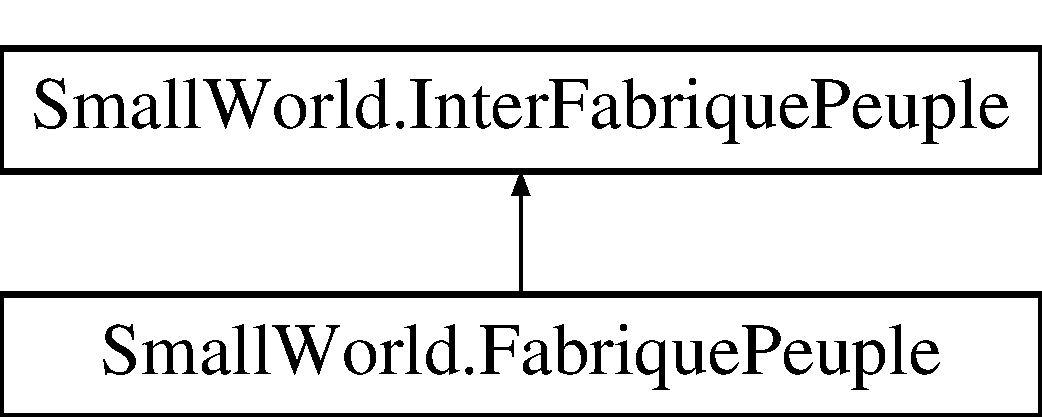
\includegraphics[height=2.000000cm]{class_small_world_1_1_fabrique_peuple}
\end{center}
\end{figure}
\subsection*{Public Member Functions}
\begin{DoxyCompactItemize}
\item 
\hypertarget{class_small_world_1_1_fabrique_peuple_a5fe5672eb02c7fb6f0aedccfe490b3b9}{\hyperlink{class_small_world_1_1_fabrique_peuple_a5fe5672eb02c7fb6f0aedccfe490b3b9}{Fabrique\-Peuple} ()}\label{class_small_world_1_1_fabrique_peuple_a5fe5672eb02c7fb6f0aedccfe490b3b9}

\begin{DoxyCompactList}\small\item\em Constructeur d'une fabrique de peuple. \end{DoxyCompactList}\item 
\hyperlink{class_small_world_1_1_peuple}{Peuple} \hyperlink{class_small_world_1_1_fabrique_peuple_ad3c21feceaebffdbfc0bdcb66edc4bdb}{fabriquer\-Peuple} (string peuple)
\begin{DoxyCompactList}\small\item\em Récupération d'un peuple. \end{DoxyCompactList}\end{DoxyCompactItemize}
\subsection*{Properties}
\begin{DoxyCompactItemize}
\item 
\hypertarget{class_small_world_1_1_fabrique_peuple_a2d46d0022cccca8e6fa8a44c097aea6a}{static \hyperlink{class_small_world_1_1_fabrique_peuple}{Fabrique\-Peuple} \hyperlink{class_small_world_1_1_fabrique_peuple_a2d46d0022cccca8e6fa8a44c097aea6a}{Instance\-\_\-\-Fab\-Peuple}\hspace{0.3cm}{\ttfamily  \mbox{[}get\mbox{]}}}\label{class_small_world_1_1_fabrique_peuple_a2d46d0022cccca8e6fa8a44c097aea6a}

\begin{DoxyCompactList}\small\item\em \hyperlink{namespace_small_world_1_1_properties}{Properties} pour l'attribut instance\-\_\-\-Fab\-Peuple. \end{DoxyCompactList}\end{DoxyCompactItemize}


\subsection{Detailed Description}
classe pour la fabrique d'un peuple 

\hyperlink{class_small_world_1_1_fabrique_peuple}{Fabrique\-Peuple} est un singleton 

\subsection{Member Function Documentation}
\hypertarget{class_small_world_1_1_fabrique_peuple_ad3c21feceaebffdbfc0bdcb66edc4bdb}{\index{Small\-World\-::\-Fabrique\-Peuple@{Small\-World\-::\-Fabrique\-Peuple}!fabriquer\-Peuple@{fabriquer\-Peuple}}
\index{fabriquer\-Peuple@{fabriquer\-Peuple}!SmallWorld::FabriquePeuple@{Small\-World\-::\-Fabrique\-Peuple}}
\subsubsection[{fabriquer\-Peuple}]{\setlength{\rightskip}{0pt plus 5cm}Small\-World.\-Fabrique\-Peuple.\-fabriquer\-Peuple (
\begin{DoxyParamCaption}
\item[{string}]{peuple}
\end{DoxyParamCaption}
)}}\label{class_small_world_1_1_fabrique_peuple_ad3c21feceaebffdbfc0bdcb66edc4bdb}


Récupération d'un peuple. 


\begin{DoxyParams}{Parameters}
{\em string} & {\bfseries peuple} le peuple demandé \\
\hline
\end{DoxyParams}
\begin{DoxyReturn}{Returns}
\hyperlink{class_small_world_1_1_peuple}{Peuple} Le peuple 
\end{DoxyReturn}


Implements \hyperlink{interface_small_world_1_1_inter_fabrique_peuple_a5f4c738231b141ffc6afd295d259a80a}{Small\-World.\-Inter\-Fabrique\-Peuple}.



The documentation for this class was generated from the following file\-:\begin{DoxyCompactItemize}
\item 
C\-:/\-Users/damienc/\-Documents/\-Git\-Hub/\-Small\-World/\-Visual\-Studio/\-Projet\-P\-O\-O/\hyperlink{_fabrique_peuple_8cs}{Fabrique\-Peuple.\-cs}\end{DoxyCompactItemize}

\hypertarget{class_small_world_1_1_foret}{\section{Small\-World.\-Foret Class Reference}
\label{class_small_world_1_1_foret}\index{Small\-World.\-Foret@{Small\-World.\-Foret}}
}
Inheritance diagram for Small\-World.\-Foret\-:\begin{figure}[H]
\begin{center}
\leavevmode
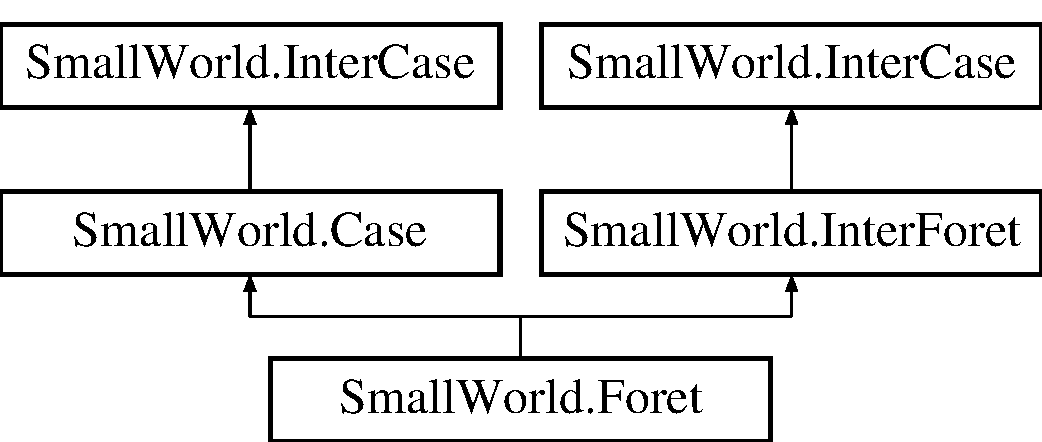
\includegraphics[height=3.000000cm]{class_small_world_1_1_foret}
\end{center}
\end{figure}


The documentation for this class was generated from the following file\-:\begin{DoxyCompactItemize}
\item 
C\-:/\-Users/damienc/\-Documents/\-Git\-Hub/\-Small\-World/\-Visual\-Studio/\-Projet\-P\-O\-O/foret.\-cs\end{DoxyCompactItemize}

\hypertarget{interface_small_world_1_1_inter_carte}{\section{Small\-World.\-Inter\-Carte Interface Reference}
\label{interface_small_world_1_1_inter_carte}\index{Small\-World.\-Inter\-Carte@{Small\-World.\-Inter\-Carte}}
}
Inheritance diagram for Small\-World.\-Inter\-Carte\-:\begin{figure}[H]
\begin{center}
\leavevmode
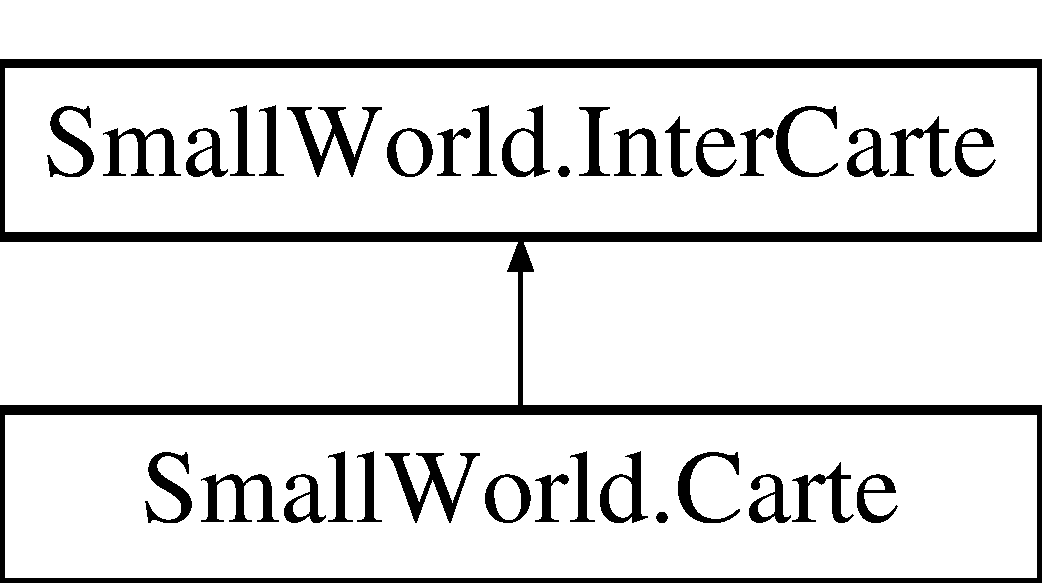
\includegraphics[height=2.000000cm]{interface_small_world_1_1_inter_carte}
\end{center}
\end{figure}
\subsection*{Public Member Functions}
\begin{DoxyCompactItemize}
\item 
\hypertarget{interface_small_world_1_1_inter_carte_aa74e8d2a86277fdd29fcf2529020f205}{void {\bfseries creer\-Carte} ()}\label{interface_small_world_1_1_inter_carte_aa74e8d2a86277fdd29fcf2529020f205}

\item 
\hypertarget{interface_small_world_1_1_inter_carte_a846d9483ff804a7e3df4584e451cc9bb}{void {\bfseries definir\-Strategie} ()}\label{interface_small_world_1_1_inter_carte_a846d9483ff804a7e3df4584e451cc9bb}

\end{DoxyCompactItemize}


The documentation for this interface was generated from the following file\-:\begin{DoxyCompactItemize}
\item 
C\-:/\-Users/damienc/\-Documents/\-Git\-Hub/\-Small\-World/\-Visual\-Studio/\-Projet\-P\-O\-O/Carte.\-cs\end{DoxyCompactItemize}

\hypertarget{interface_small_world_1_1_inter_case}{\section{Small\-World.\-Inter\-Case Interface Reference}
\label{interface_small_world_1_1_inter_case}\index{Small\-World.\-Inter\-Case@{Small\-World.\-Inter\-Case}}
}
Inheritance diagram for Small\-World.\-Inter\-Case\-:\begin{figure}[H]
\begin{center}
\leavevmode
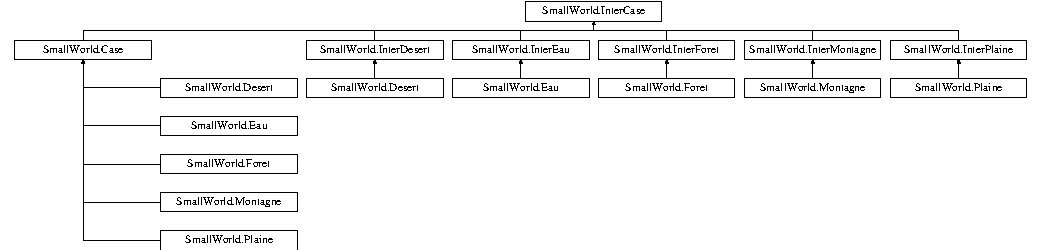
\includegraphics[height=3.333333cm]{interface_small_world_1_1_inter_case}
\end{center}
\end{figure}


The documentation for this interface was generated from the following file\-:\begin{DoxyCompactItemize}
\item 
C\-:/\-Users/damienc/\-Documents/\-Git\-Hub/\-Small\-World/\-Visual\-Studio/\-Projet\-P\-O\-O/Case.\-cs\end{DoxyCompactItemize}

\hypertarget{interface_inter_coordonnees}{\section{Inter\-Coordonnees Interface Reference}
\label{interface_inter_coordonnees}\index{Inter\-Coordonnees@{Inter\-Coordonnees}}
}


Interface pour Coordonnees.  




\subsection{Detailed Description}
Interface pour Coordonnees. 

The documentation for this interface was generated from the following file\-:\begin{DoxyCompactItemize}
\item 
C\-:/\-Users/damienc/\-Documents/\-Git\-Hub/\-Small\-World/\-Visual\-Studio/\-Projet\-P\-O\-O/\hyperlink{_coordonnees_8cs}{Coordonnees.\-cs}\end{DoxyCompactItemize}

\hypertarget{interface_small_world_1_1_inter_cordonnees}{\section{Small\-World.\-Inter\-Cordonnees Interface Reference}
\label{interface_small_world_1_1_inter_cordonnees}\index{Small\-World.\-Inter\-Cordonnees@{Small\-World.\-Inter\-Cordonnees}}
}
Inheritance diagram for Small\-World.\-Inter\-Cordonnees\-:\begin{figure}[H]
\begin{center}
\leavevmode
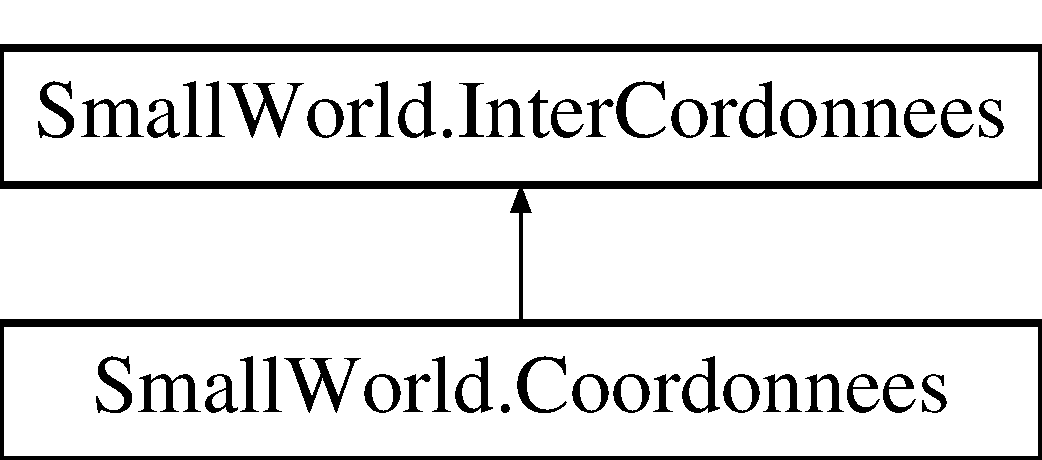
\includegraphics[height=2.000000cm]{interface_small_world_1_1_inter_cordonnees}
\end{center}
\end{figure}


The documentation for this interface was generated from the following file\-:\begin{DoxyCompactItemize}
\item 
C\-:/\-Users/damienc/\-Documents/\-Git\-Hub/\-Small\-World/\-Visual\-Studio/\-Projet\-P\-O\-O/\hyperlink{_coordonnees_8cs}{Coordonnees.\-cs}\end{DoxyCompactItemize}

\hypertarget{interface_small_world_1_1_inter_createur_partie}{\section{Small\-World.\-Inter\-Createur\-Partie Interface Reference}
\label{interface_small_world_1_1_inter_createur_partie}\index{Small\-World.\-Inter\-Createur\-Partie@{Small\-World.\-Inter\-Createur\-Partie}}
}


Interface du créateur de partie.  


Inheritance diagram for Small\-World.\-Inter\-Createur\-Partie\-:\begin{figure}[H]
\begin{center}
\leavevmode
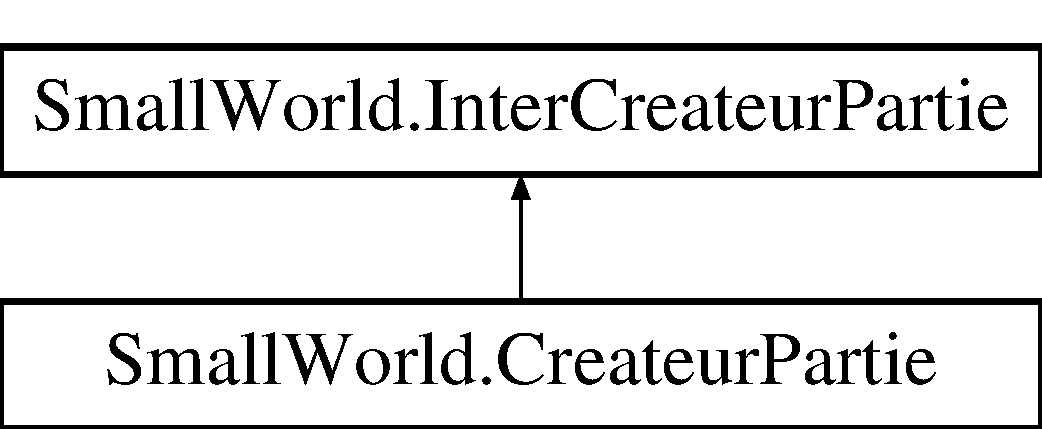
\includegraphics[height=2.000000cm]{interface_small_world_1_1_inter_createur_partie}
\end{center}
\end{figure}
\subsection*{Public Member Functions}
\begin{DoxyCompactItemize}
\item 
\hypertarget{interface_small_world_1_1_inter_createur_partie_a84bc048d2a71699fef54ef531477c917}{\hyperlink{class_small_world_1_1_partie}{Partie} \hyperlink{interface_small_world_1_1_inter_createur_partie_a84bc048d2a71699fef54ef531477c917}{construire} ()}\label{interface_small_world_1_1_inter_createur_partie_a84bc048d2a71699fef54ef531477c917}

\begin{DoxyCompactList}\small\item\em Construire la partie. \end{DoxyCompactList}\item 
void \hyperlink{interface_small_world_1_1_inter_createur_partie_af3fa5aaff01c6709b99eff93b6252da5}{ajout\-Joueur} (string nom, string peuple)
\begin{DoxyCompactList}\small\item\em Ajouter un joueur à la partie. \end{DoxyCompactList}\end{DoxyCompactItemize}


\subsection{Detailed Description}
Interface du créateur de partie. 

\subsection{Member Function Documentation}
\hypertarget{interface_small_world_1_1_inter_createur_partie_af3fa5aaff01c6709b99eff93b6252da5}{\index{Small\-World\-::\-Inter\-Createur\-Partie@{Small\-World\-::\-Inter\-Createur\-Partie}!ajout\-Joueur@{ajout\-Joueur}}
\index{ajout\-Joueur@{ajout\-Joueur}!SmallWorld::InterCreateurPartie@{Small\-World\-::\-Inter\-Createur\-Partie}}
\subsubsection[{ajout\-Joueur}]{\setlength{\rightskip}{0pt plus 5cm}Small\-World.\-Inter\-Createur\-Partie.\-ajout\-Joueur (
\begin{DoxyParamCaption}
\item[{string}]{nom, }
\item[{string}]{peuple}
\end{DoxyParamCaption}
)}}\label{interface_small_world_1_1_inter_createur_partie_af3fa5aaff01c6709b99eff93b6252da5}


Ajouter un joueur à la partie. 


\begin{DoxyParams}{Parameters}
{\em string} & {\bfseries nom} le nom du joueur \\
\hline
{\em string} & {\bfseries peuple} le type de peuple \\
\hline
\end{DoxyParams}
\begin{DoxyReturn}{Returns}
void 
\end{DoxyReturn}


Implemented in \hyperlink{class_small_world_1_1_createur_partie_a1388144440304d2d82879a15e0e58e1f}{Small\-World.\-Createur\-Partie}.



The documentation for this interface was generated from the following file\-:\begin{DoxyCompactItemize}
\item 
C\-:/\-Users/damienc/\-Documents/\-Git\-Hub/\-Small\-World/\-Visual\-Studio/\-Projet\-P\-O\-O/\hyperlink{_createur_partie_8cs}{Createur\-Partie.\-cs}\end{DoxyCompactItemize}

\hypertarget{interface_small_world_1_1_inter_desert}{\section{Small\-World.\-Inter\-Desert Interface Reference}
\label{interface_small_world_1_1_inter_desert}\index{Small\-World.\-Inter\-Desert@{Small\-World.\-Inter\-Desert}}
}
Inheritance diagram for Small\-World.\-Inter\-Desert\-:\begin{figure}[H]
\begin{center}
\leavevmode
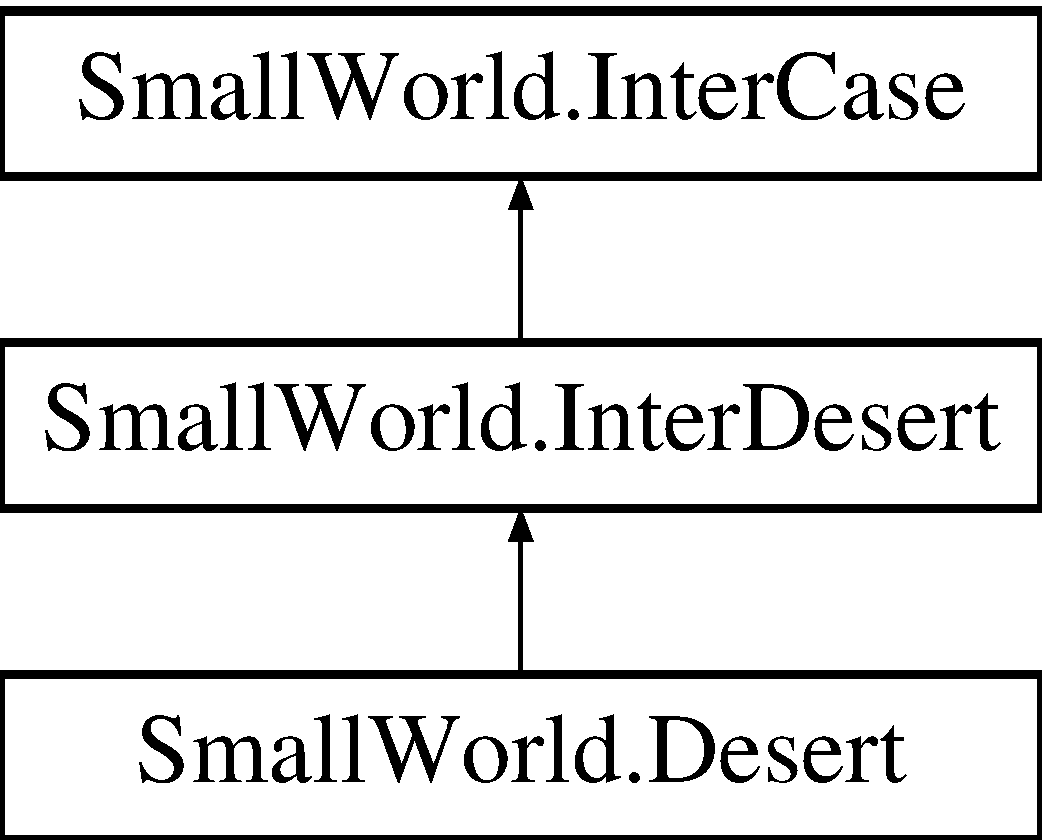
\includegraphics[height=3.000000cm]{interface_small_world_1_1_inter_desert}
\end{center}
\end{figure}


The documentation for this interface was generated from the following file\-:\begin{DoxyCompactItemize}
\item 
C\-:/\-Users/damienc/\-Documents/\-Git\-Hub/\-Small\-World/\-Visual\-Studio/\-Projet\-P\-O\-O/Case.\-cs\end{DoxyCompactItemize}

\hypertarget{interface_small_world_1_1_inter_eau}{\section{Small\-World.\-Inter\-Eau Interface Reference}
\label{interface_small_world_1_1_inter_eau}\index{Small\-World.\-Inter\-Eau@{Small\-World.\-Inter\-Eau}}
}
Inheritance diagram for Small\-World.\-Inter\-Eau\-:\begin{figure}[H]
\begin{center}
\leavevmode
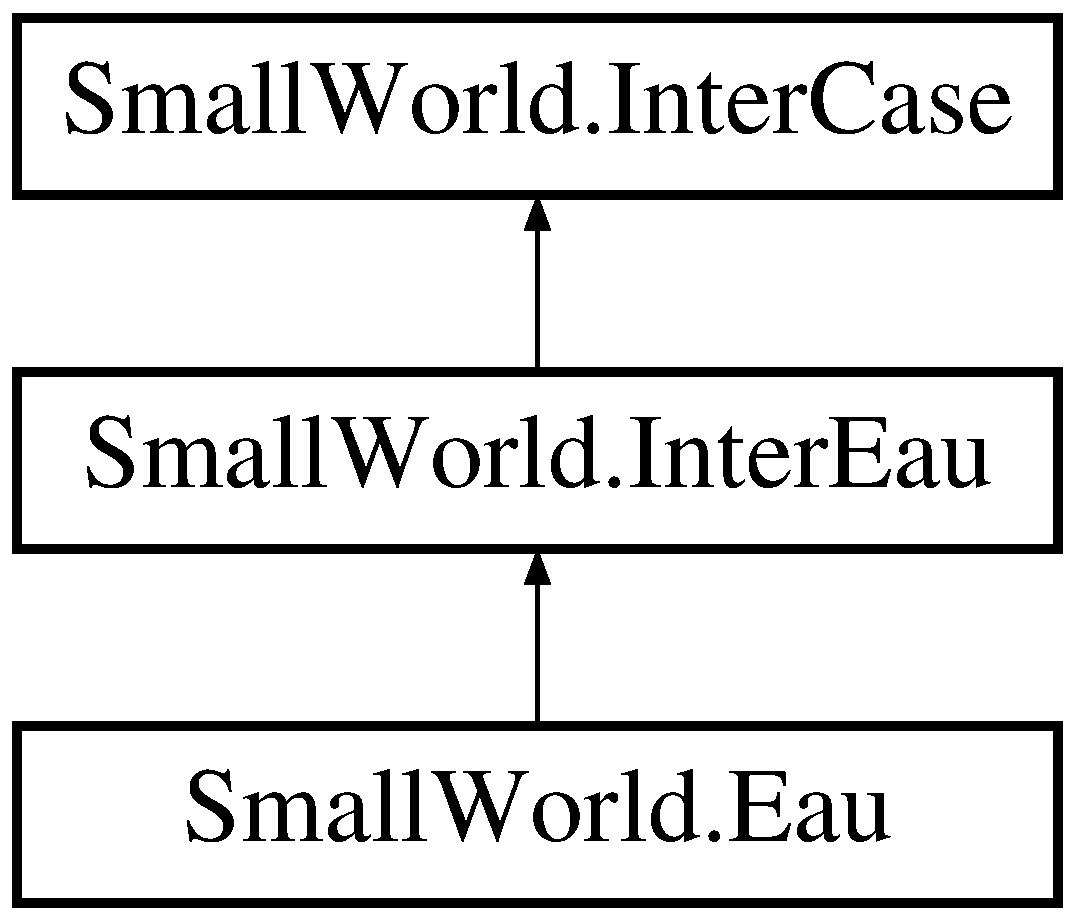
\includegraphics[height=3.000000cm]{interface_small_world_1_1_inter_eau}
\end{center}
\end{figure}


The documentation for this interface was generated from the following file\-:\begin{DoxyCompactItemize}
\item 
C\-:/\-Users/damienc/\-Documents/\-Git\-Hub/\-Small\-World/\-Visual\-Studio/\-Projet\-P\-O\-O/Case.\-cs\end{DoxyCompactItemize}

\hypertarget{interface_small_world_1_1_inter_fabrique_case}{\section{Small\-World.\-Inter\-Fabrique\-Case Interface Reference}
\label{interface_small_world_1_1_inter_fabrique_case}\index{Small\-World.\-Inter\-Fabrique\-Case@{Small\-World.\-Inter\-Fabrique\-Case}}
}
Inheritance diagram for Small\-World.\-Inter\-Fabrique\-Case\-:\begin{figure}[H]
\begin{center}
\leavevmode
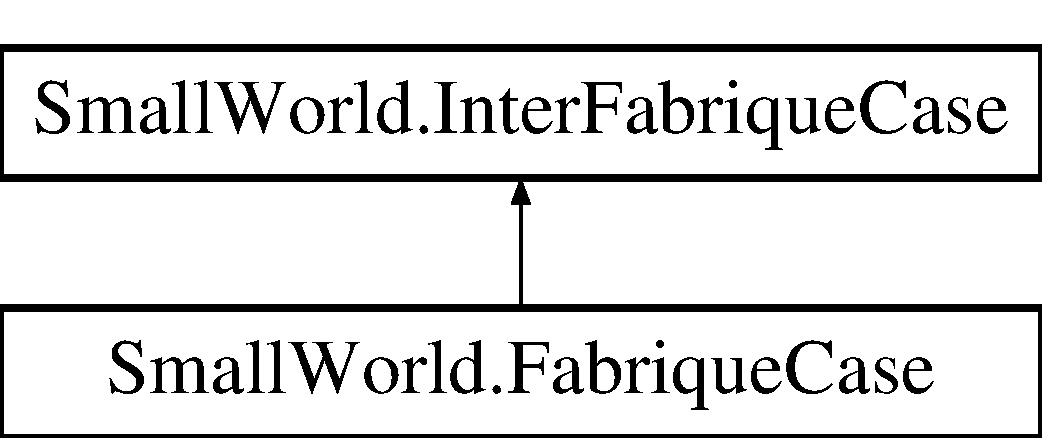
\includegraphics[height=2.000000cm]{interface_small_world_1_1_inter_fabrique_case}
\end{center}
\end{figure}
\subsection*{Public Member Functions}
\begin{DoxyCompactItemize}
\item 
\hypertarget{interface_small_world_1_1_inter_fabrique_case_a1434bcec9bf29cfd87d80bb0b71c709c}{\hyperlink{class_small_world_1_1_case}{Case} {\bfseries obtenir\-Eau} ()}\label{interface_small_world_1_1_inter_fabrique_case_a1434bcec9bf29cfd87d80bb0b71c709c}

\item 
\hypertarget{interface_small_world_1_1_inter_fabrique_case_af726293fdccaa7f5af1729551a6dd1ed}{\hyperlink{class_small_world_1_1_case}{Case} {\bfseries obtenir\-Montagne} ()}\label{interface_small_world_1_1_inter_fabrique_case_af726293fdccaa7f5af1729551a6dd1ed}

\item 
\hypertarget{interface_small_world_1_1_inter_fabrique_case_a9ffa841ddec5636b3241db2e4cf51b49}{\hyperlink{class_small_world_1_1_case}{Case} {\bfseries obtenir\-Desert} ()}\label{interface_small_world_1_1_inter_fabrique_case_a9ffa841ddec5636b3241db2e4cf51b49}

\item 
\hypertarget{interface_small_world_1_1_inter_fabrique_case_a8f35df965c3546307d905b2909dca774}{\hyperlink{class_small_world_1_1_case}{Case} {\bfseries obtenir\-Plaine} ()}\label{interface_small_world_1_1_inter_fabrique_case_a8f35df965c3546307d905b2909dca774}

\item 
\hypertarget{interface_small_world_1_1_inter_fabrique_case_aaf69be0da8fc845f9e8418e028cf41fc}{\hyperlink{class_small_world_1_1_case}{Case} {\bfseries obtenir\-Foret} ()}\label{interface_small_world_1_1_inter_fabrique_case_aaf69be0da8fc845f9e8418e028cf41fc}

\item 
\hypertarget{interface_small_world_1_1_inter_fabrique_case_a67a341c2ee1caef98513b5fe701e953b}{\hyperlink{class_small_world_1_1_case}{Case} {\bfseries obtenir\-Case} (int type\-Case)}\label{interface_small_world_1_1_inter_fabrique_case_a67a341c2ee1caef98513b5fe701e953b}

\end{DoxyCompactItemize}


The documentation for this interface was generated from the following file\-:\begin{DoxyCompactItemize}
\item 
C\-:/\-Users/damienc/\-Documents/\-Git\-Hub/\-Small\-World/\-Visual\-Studio/\-Projet\-P\-O\-O/Fabrique\-Case.\-cs\end{DoxyCompactItemize}

\hypertarget{interface_small_world_1_1_inter_fabrique_peuple}{\section{Small\-World.\-Inter\-Fabrique\-Peuple Interface Reference}
\label{interface_small_world_1_1_inter_fabrique_peuple}\index{Small\-World.\-Inter\-Fabrique\-Peuple@{Small\-World.\-Inter\-Fabrique\-Peuple}}
}
Inheritance diagram for Small\-World.\-Inter\-Fabrique\-Peuple\-:\begin{figure}[H]
\begin{center}
\leavevmode
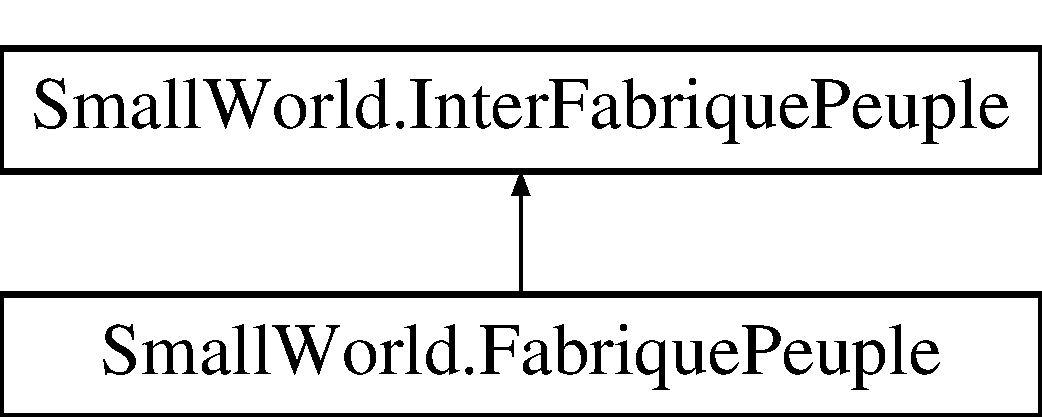
\includegraphics[height=1.266968cm]{interface_small_world_1_1_inter_fabrique_peuple}
\end{center}
\end{figure}
\subsection*{Public Member Functions}
\begin{DoxyCompactItemize}
\item 
\hypertarget{interface_small_world_1_1_inter_fabrique_peuple_a43c849b7b035e7ebf2e96128c75cd0ee}{void {\bfseries fabriquer\-Peuple} ()}\label{interface_small_world_1_1_inter_fabrique_peuple_a43c849b7b035e7ebf2e96128c75cd0ee}

\end{DoxyCompactItemize}


The documentation for this interface was generated from the following file\-:\begin{DoxyCompactItemize}
\item 
C\-:/\-Users/damienc/\-Documents/\-Git\-Hub/\-Small\-World/\-Visual\-Studio/\-Projet\-P\-O\-O/Fabrique.\-cs\end{DoxyCompactItemize}

\hypertarget{interface_small_world_1_1_inter_foret}{\section{Small\-World.\-Inter\-Foret Interface Reference}
\label{interface_small_world_1_1_inter_foret}\index{Small\-World.\-Inter\-Foret@{Small\-World.\-Inter\-Foret}}
}
Inheritance diagram for Small\-World.\-Inter\-Foret\-:\begin{figure}[H]
\begin{center}
\leavevmode
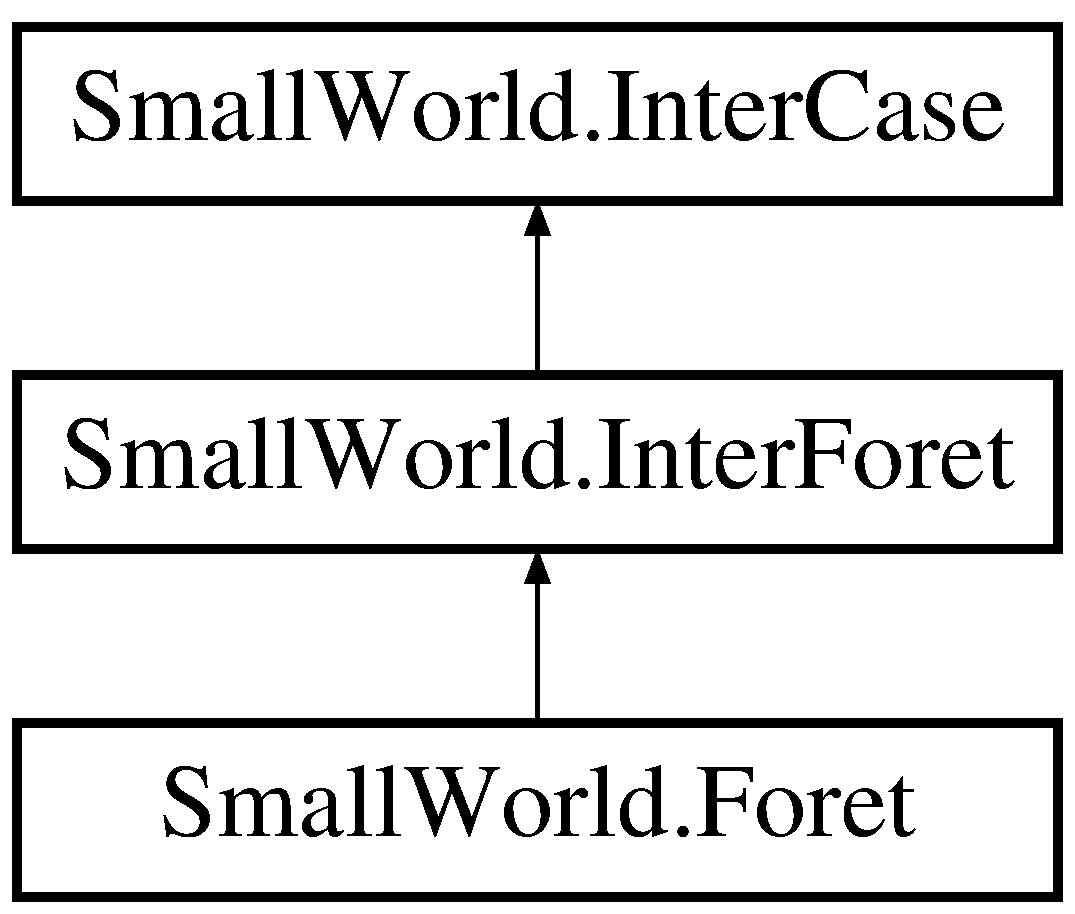
\includegraphics[height=3.000000cm]{interface_small_world_1_1_inter_foret}
\end{center}
\end{figure}


The documentation for this interface was generated from the following file\-:\begin{DoxyCompactItemize}
\item 
C\-:/\-Users/damienc/\-Documents/\-Git\-Hub/\-Small\-World/\-Visual\-Studio/\-Projet\-P\-O\-O/Case.\-cs\end{DoxyCompactItemize}

\hypertarget{interface_small_world_1_1_inter_joueur}{\section{Small\-World.\-Inter\-Joueur Interface Reference}
\label{interface_small_world_1_1_inter_joueur}\index{Small\-World.\-Inter\-Joueur@{Small\-World.\-Inter\-Joueur}}
}


interface pour un joueur  


Inheritance diagram for Small\-World.\-Inter\-Joueur\-:\begin{figure}[H]
\begin{center}
\leavevmode
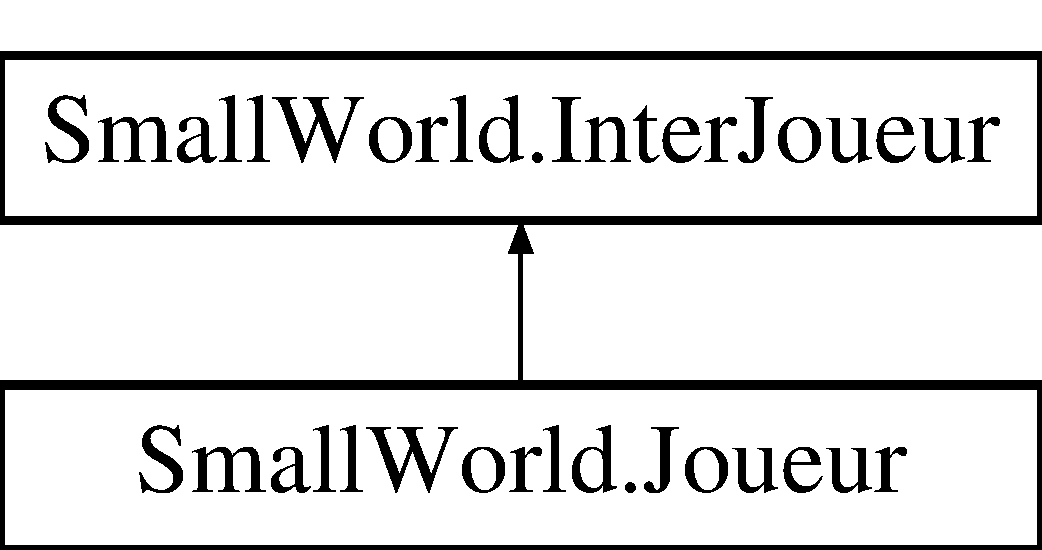
\includegraphics[height=2.000000cm]{interface_small_world_1_1_inter_joueur}
\end{center}
\end{figure}
\subsection*{Public Member Functions}
\begin{DoxyCompactItemize}
\item 
void \hyperlink{interface_small_world_1_1_inter_joueur_affcd2a1f3208993fd9fd5f78b4873b70}{calculer\-Point\-Victoire} ()
\begin{DoxyCompactList}\small\item\em Met à jour les points de victoire du joueur. \end{DoxyCompactList}\end{DoxyCompactItemize}


\subsection{Detailed Description}
interface pour un joueur 

\subsection{Member Function Documentation}
\hypertarget{interface_small_world_1_1_inter_joueur_affcd2a1f3208993fd9fd5f78b4873b70}{\index{Small\-World\-::\-Inter\-Joueur@{Small\-World\-::\-Inter\-Joueur}!calculer\-Point\-Victoire@{calculer\-Point\-Victoire}}
\index{calculer\-Point\-Victoire@{calculer\-Point\-Victoire}!SmallWorld::InterJoueur@{Small\-World\-::\-Inter\-Joueur}}
\subsubsection[{calculer\-Point\-Victoire}]{\setlength{\rightskip}{0pt plus 5cm}Small\-World.\-Inter\-Joueur.\-calculer\-Point\-Victoire (
\begin{DoxyParamCaption}
{}
\end{DoxyParamCaption}
)}}\label{interface_small_world_1_1_inter_joueur_affcd2a1f3208993fd9fd5f78b4873b70}


Met à jour les points de victoire du joueur. 

\begin{DoxyReturn}{Returns}
void 
\end{DoxyReturn}


Implemented in \hyperlink{class_small_world_1_1_joueur_aaa0f98cea097955f2c75e978433a7c68}{Small\-World.\-Joueur}.



The documentation for this interface was generated from the following file\-:\begin{DoxyCompactItemize}
\item 
C\-:/\-Users/damienc/\-Documents/\-Git\-Hub/\-Small\-World/\-Visual\-Studio/\-Projet\-P\-O\-O/\hyperlink{_joueur_8cs}{Joueur.\-cs}\end{DoxyCompactItemize}

\hypertarget{interface_small_world_1_1_inter_montagne}{\section{Small\-World.\-Inter\-Montagne Interface Reference}
\label{interface_small_world_1_1_inter_montagne}\index{Small\-World.\-Inter\-Montagne@{Small\-World.\-Inter\-Montagne}}
}
Inheritance diagram for Small\-World.\-Inter\-Montagne\-:\begin{figure}[H]
\begin{center}
\leavevmode
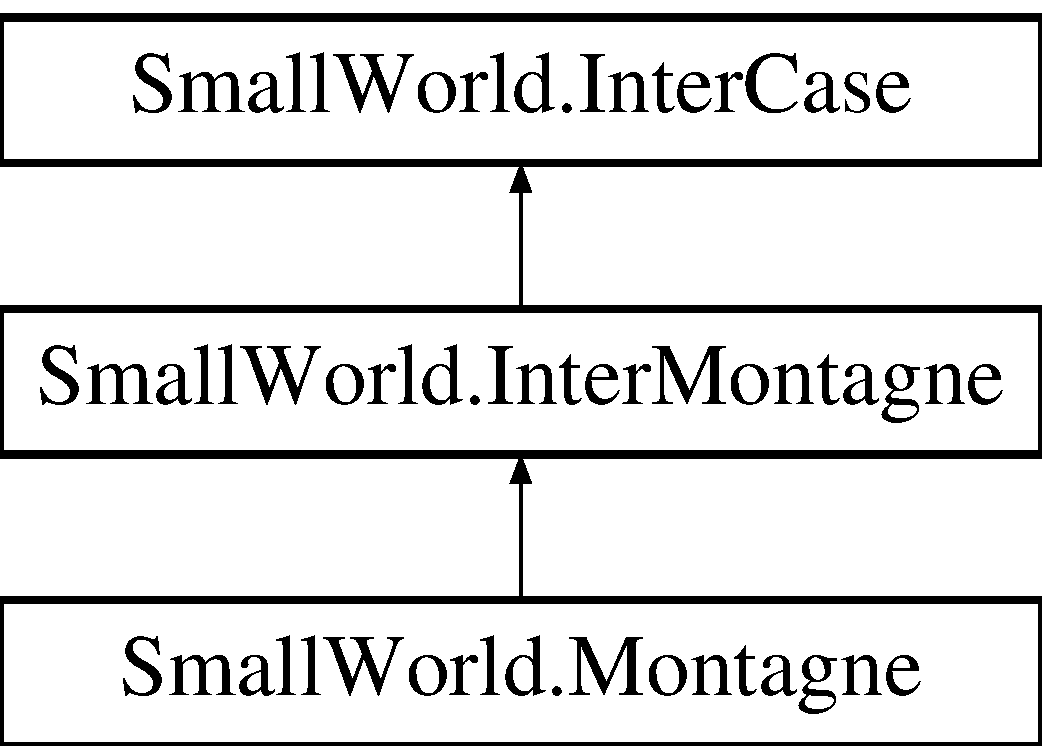
\includegraphics[height=3.000000cm]{interface_small_world_1_1_inter_montagne}
\end{center}
\end{figure}


The documentation for this interface was generated from the following file\-:\begin{DoxyCompactItemize}
\item 
C\-:/\-Users/damienc/\-Documents/\-Git\-Hub/\-Small\-World/\-Visual\-Studio/\-Projet\-P\-O\-O/Case.\-cs\end{DoxyCompactItemize}

\hypertarget{interface_small_world_1_1_inter_monteur_partie}{\section{Small\-World.\-Inter\-Monteur\-Partie Interface Reference}
\label{interface_small_world_1_1_inter_monteur_partie}\index{Small\-World.\-Inter\-Monteur\-Partie@{Small\-World.\-Inter\-Monteur\-Partie}}
}


Interface globale du monteur.  


Inheritance diagram for Small\-World.\-Inter\-Monteur\-Partie\-:\begin{figure}[H]
\begin{center}
\leavevmode
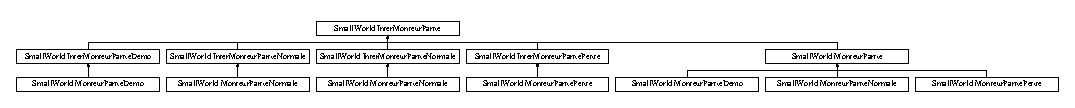
\includegraphics[height=1.171548cm]{interface_small_world_1_1_inter_monteur_partie}
\end{center}
\end{figure}
\subsection*{Public Member Functions}
\begin{DoxyCompactItemize}
\item 
void \hyperlink{interface_small_world_1_1_inter_monteur_partie_a473c91ad26ee485f07261df1fcae0e8b}{ajouter\-Carte} ()
\begin{DoxyCompactList}\small\item\em Ajout de la carte pour la construction d'une partie. \end{DoxyCompactList}\item 
void \hyperlink{interface_small_world_1_1_inter_monteur_partie_ae52498262dd36230b0c0d090cb59ff07}{ajouter\-Joueur} (string nom\-Joueur, string peuple)
\begin{DoxyCompactList}\small\item\em Ajout d'un joueur à la partie. \end{DoxyCompactList}\item 
\hyperlink{class_small_world_1_1_partie}{Partie} \hyperlink{interface_small_world_1_1_inter_monteur_partie_ad471ab6610aaa1664fb3d0bd93f00be3}{creer\-Partie} (string nom\-Joueur\-A, string peuple\-A, string nom\-Joueur\-B, string peuple\-B)
\begin{DoxyCompactList}\small\item\em Création de la partie. \end{DoxyCompactList}\item 
void \hyperlink{interface_small_world_1_1_inter_monteur_partie_a4ea7442b592d23a0f31e0d0020f124de}{placer\-Unites} ()
\begin{DoxyCompactList}\small\item\em Placement des unités avant le début de la partie. \end{DoxyCompactList}\item 
void \hyperlink{interface_small_world_1_1_inter_monteur_partie_afa1b718338a15b4dd0deb5d817f3484c}{initialiser\-Nombre\-Tour} ()
\begin{DoxyCompactList}\small\item\em initialise le nombre de tour d'un partie \end{DoxyCompactList}\end{DoxyCompactItemize}


\subsection{Detailed Description}
Interface globale du monteur. 

\subsection{Member Function Documentation}
\hypertarget{interface_small_world_1_1_inter_monteur_partie_a473c91ad26ee485f07261df1fcae0e8b}{\index{Small\-World\-::\-Inter\-Monteur\-Partie@{Small\-World\-::\-Inter\-Monteur\-Partie}!ajouter\-Carte@{ajouter\-Carte}}
\index{ajouter\-Carte@{ajouter\-Carte}!SmallWorld::InterMonteurPartie@{Small\-World\-::\-Inter\-Monteur\-Partie}}
\subsubsection[{ajouter\-Carte}]{\setlength{\rightskip}{0pt plus 5cm}Small\-World.\-Inter\-Monteur\-Partie.\-ajouter\-Carte (
\begin{DoxyParamCaption}
{}
\end{DoxyParamCaption}
)}}\label{interface_small_world_1_1_inter_monteur_partie_a473c91ad26ee485f07261df1fcae0e8b}


Ajout de la carte pour la construction d'une partie. 

\begin{DoxyReturn}{Returns}
void 
\end{DoxyReturn}


Implemented in \hyperlink{class_small_world_1_1_monteur_partie_ad8cedb326193c0f0ff5f2d6705867156}{Small\-World.\-Monteur\-Partie}.

\hypertarget{interface_small_world_1_1_inter_monteur_partie_ae52498262dd36230b0c0d090cb59ff07}{\index{Small\-World\-::\-Inter\-Monteur\-Partie@{Small\-World\-::\-Inter\-Monteur\-Partie}!ajouter\-Joueur@{ajouter\-Joueur}}
\index{ajouter\-Joueur@{ajouter\-Joueur}!SmallWorld::InterMonteurPartie@{Small\-World\-::\-Inter\-Monteur\-Partie}}
\subsubsection[{ajouter\-Joueur}]{\setlength{\rightskip}{0pt plus 5cm}Small\-World.\-Inter\-Monteur\-Partie.\-ajouter\-Joueur (
\begin{DoxyParamCaption}
\item[{string}]{nom\-Joueur, }
\item[{string}]{peuple}
\end{DoxyParamCaption}
)}}\label{interface_small_world_1_1_inter_monteur_partie_ae52498262dd36230b0c0d090cb59ff07}


Ajout d'un joueur à la partie. 


\begin{DoxyParams}{Parameters}
{\em string} & {\bfseries nom\-Joueur} Le nom du joueur à ajouter. \\
\hline
{\em string} & {\bfseries peuple} Le peuple joué par le joueur. \\
\hline
\end{DoxyParams}
\begin{DoxyReturn}{Returns}
void 
\end{DoxyReturn}


Implemented in \hyperlink{class_small_world_1_1_monteur_partie_ac1e20f04d1ca796c1aa0ab504ecb1d2a}{Small\-World.\-Monteur\-Partie}.

\hypertarget{interface_small_world_1_1_inter_monteur_partie_ad471ab6610aaa1664fb3d0bd93f00be3}{\index{Small\-World\-::\-Inter\-Monteur\-Partie@{Small\-World\-::\-Inter\-Monteur\-Partie}!creer\-Partie@{creer\-Partie}}
\index{creer\-Partie@{creer\-Partie}!SmallWorld::InterMonteurPartie@{Small\-World\-::\-Inter\-Monteur\-Partie}}
\subsubsection[{creer\-Partie}]{\setlength{\rightskip}{0pt plus 5cm}Small\-World.\-Inter\-Monteur\-Partie.\-creer\-Partie (
\begin{DoxyParamCaption}
\item[{string}]{nom\-Joueur\-A, }
\item[{string}]{peuple\-A, }
\item[{string}]{nom\-Joueur\-B, }
\item[{string}]{peuple\-B}
\end{DoxyParamCaption}
)}}\label{interface_small_world_1_1_inter_monteur_partie_ad471ab6610aaa1664fb3d0bd93f00be3}


Création de la partie. 


\begin{DoxyParams}{Parameters}
{\em string} & {\bfseries nom\-Joueur\-A} le nom du premier joueur \\
\hline
{\em string} & {\bfseries peuple\-A} le peuple du premier joueur \\
\hline
{\em string} & {\bfseries nom\-Joueur\-B} le nom du deuxième joueur \\
\hline
{\em string} & {\bfseries peuple\-B} le peuple du deuxième joueur \\
\hline
\end{DoxyParams}
\begin{DoxyReturn}{Returns}
\hyperlink{class_small_world_1_1_partie}{Partie} la nouvelle partie 
\end{DoxyReturn}


Implemented in \hyperlink{class_small_world_1_1_monteur_partie_a76b953c2a45b0c3355d764355d85e225}{Small\-World.\-Monteur\-Partie}.

\hypertarget{interface_small_world_1_1_inter_monteur_partie_afa1b718338a15b4dd0deb5d817f3484c}{\index{Small\-World\-::\-Inter\-Monteur\-Partie@{Small\-World\-::\-Inter\-Monteur\-Partie}!initialiser\-Nombre\-Tour@{initialiser\-Nombre\-Tour}}
\index{initialiser\-Nombre\-Tour@{initialiser\-Nombre\-Tour}!SmallWorld::InterMonteurPartie@{Small\-World\-::\-Inter\-Monteur\-Partie}}
\subsubsection[{initialiser\-Nombre\-Tour}]{\setlength{\rightskip}{0pt plus 5cm}Small\-World.\-Inter\-Monteur\-Partie.\-initialiser\-Nombre\-Tour (
\begin{DoxyParamCaption}
{}
\end{DoxyParamCaption}
)}}\label{interface_small_world_1_1_inter_monteur_partie_afa1b718338a15b4dd0deb5d817f3484c}


initialise le nombre de tour d'un partie 

\begin{DoxyReturn}{Returns}
void 
\end{DoxyReturn}


Implemented in \hyperlink{class_small_world_1_1_monteur_partie_a8bfe459f9efcb0561a7612e720e0a373}{Small\-World.\-Monteur\-Partie}.

\hypertarget{interface_small_world_1_1_inter_monteur_partie_a4ea7442b592d23a0f31e0d0020f124de}{\index{Small\-World\-::\-Inter\-Monteur\-Partie@{Small\-World\-::\-Inter\-Monteur\-Partie}!placer\-Unites@{placer\-Unites}}
\index{placer\-Unites@{placer\-Unites}!SmallWorld::InterMonteurPartie@{Small\-World\-::\-Inter\-Monteur\-Partie}}
\subsubsection[{placer\-Unites}]{\setlength{\rightskip}{0pt plus 5cm}Small\-World.\-Inter\-Monteur\-Partie.\-placer\-Unites (
\begin{DoxyParamCaption}
{}
\end{DoxyParamCaption}
)}}\label{interface_small_world_1_1_inter_monteur_partie_a4ea7442b592d23a0f31e0d0020f124de}


Placement des unités avant le début de la partie. 

\begin{DoxyReturn}{Returns}
void 
\end{DoxyReturn}


Implemented in \hyperlink{class_small_world_1_1_monteur_partie_a5cba1ab3dd04f490331bf22e540cc80e}{Small\-World.\-Monteur\-Partie}.



The documentation for this interface was generated from the following file\-:\begin{DoxyCompactItemize}
\item 
C\-:/\-Users/damienc/\-Documents/\-Git\-Hub/\-Small\-World/\-Visual\-Studio/\-Projet\-P\-O\-O/\hyperlink{_monteur_partie_8cs}{Monteur\-Partie.\-cs}\end{DoxyCompactItemize}

\hypertarget{interface_small_world_1_1_inter_monteur_partie_demo}{\section{Small\-World.\-Inter\-Monteur\-Partie\-Demo Interface Reference}
\label{interface_small_world_1_1_inter_monteur_partie_demo}\index{Small\-World.\-Inter\-Monteur\-Partie\-Demo@{Small\-World.\-Inter\-Monteur\-Partie\-Demo}}
}


Interface du monteur de partie démo.  


Inheritance diagram for Small\-World.\-Inter\-Monteur\-Partie\-Demo\-:\begin{figure}[H]
\begin{center}
\leavevmode
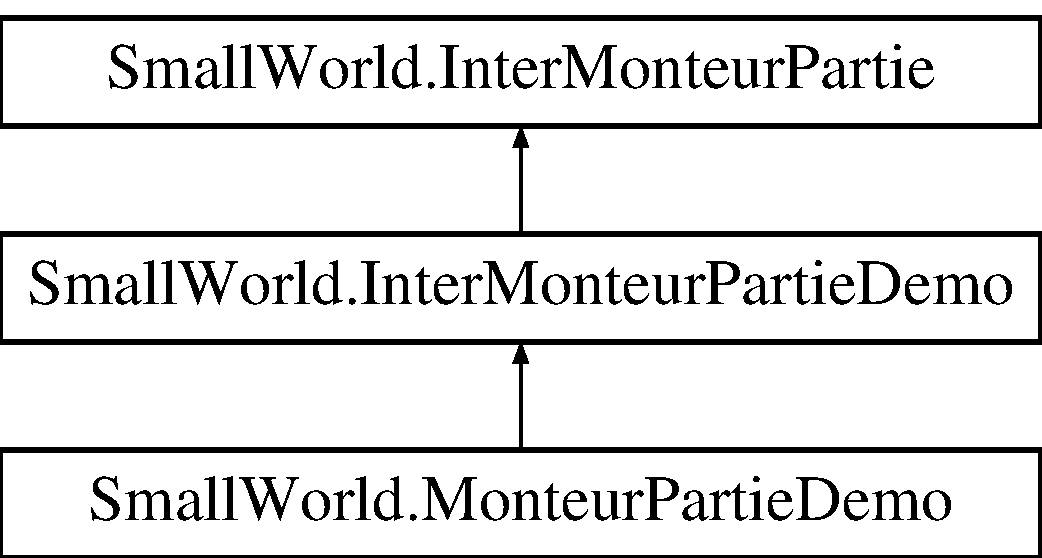
\includegraphics[height=3.000000cm]{interface_small_world_1_1_inter_monteur_partie_demo}
\end{center}
\end{figure}
\subsection*{Additional Inherited Members}


\subsection{Detailed Description}
Interface du monteur de partie démo. 

The documentation for this interface was generated from the following file\-:\begin{DoxyCompactItemize}
\item 
C\-:/\-Users/damienc/\-Documents/\-Git\-Hub/\-Small\-World/\-Visual\-Studio/\-Projet\-P\-O\-O/\hyperlink{_monteur_partie_8cs}{Monteur\-Partie.\-cs}\end{DoxyCompactItemize}

\hypertarget{interface_small_world_1_1_inter_monteur_partie_normale}{\section{Small\-World.\-Inter\-Monteur\-Partie\-Normale Interface Reference}
\label{interface_small_world_1_1_inter_monteur_partie_normale}\index{Small\-World.\-Inter\-Monteur\-Partie\-Normale@{Small\-World.\-Inter\-Monteur\-Partie\-Normale}}
}
Inheritance diagram for Small\-World.\-Inter\-Monteur\-Partie\-Normale\-:\begin{figure}[H]
\begin{center}
\leavevmode
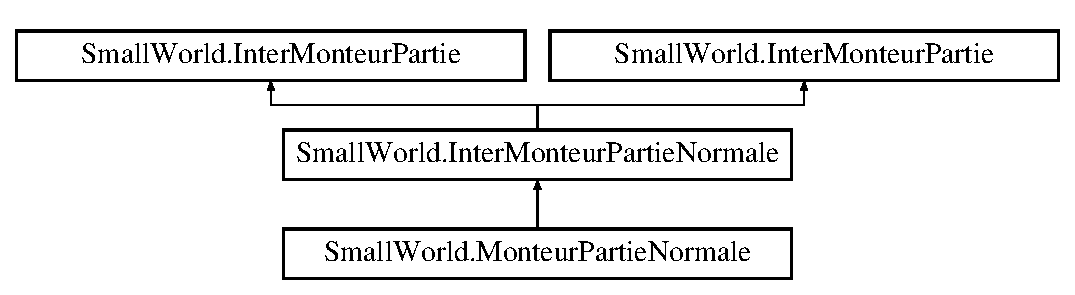
\includegraphics[height=3.000000cm]{interface_small_world_1_1_inter_monteur_partie_normale}
\end{center}
\end{figure}
\subsection*{Public Member Functions}
\begin{DoxyCompactItemize}
\item 
\hypertarget{interface_small_world_1_1_inter_monteur_partie_normale_a4616843a525be26a4d55e3928f21ef3d}{void {\bfseries ajouter\-Peuple} ()}\label{interface_small_world_1_1_inter_monteur_partie_normale_a4616843a525be26a4d55e3928f21ef3d}

\end{DoxyCompactItemize}


The documentation for this interface was generated from the following file\-:\begin{DoxyCompactItemize}
\item 
C\-:/\-Users/damienc/\-Documents/\-Git\-Hub/\-Small\-World/\-Visual\-Studio/\-Projet\-P\-O\-O/\hyperlink{_monteur_partie_8cs}{Monteur\-Partie.\-cs}\end{DoxyCompactItemize}

\hypertarget{interface_small_world_1_1_inter_monteur_partie_petite}{\section{Small\-World.\-Inter\-Monteur\-Partie\-Petite Interface Reference}
\label{interface_small_world_1_1_inter_monteur_partie_petite}\index{Small\-World.\-Inter\-Monteur\-Partie\-Petite@{Small\-World.\-Inter\-Monteur\-Partie\-Petite}}
}
Inheritance diagram for Small\-World.\-Inter\-Monteur\-Partie\-Petite\-:\begin{figure}[H]
\begin{center}
\leavevmode
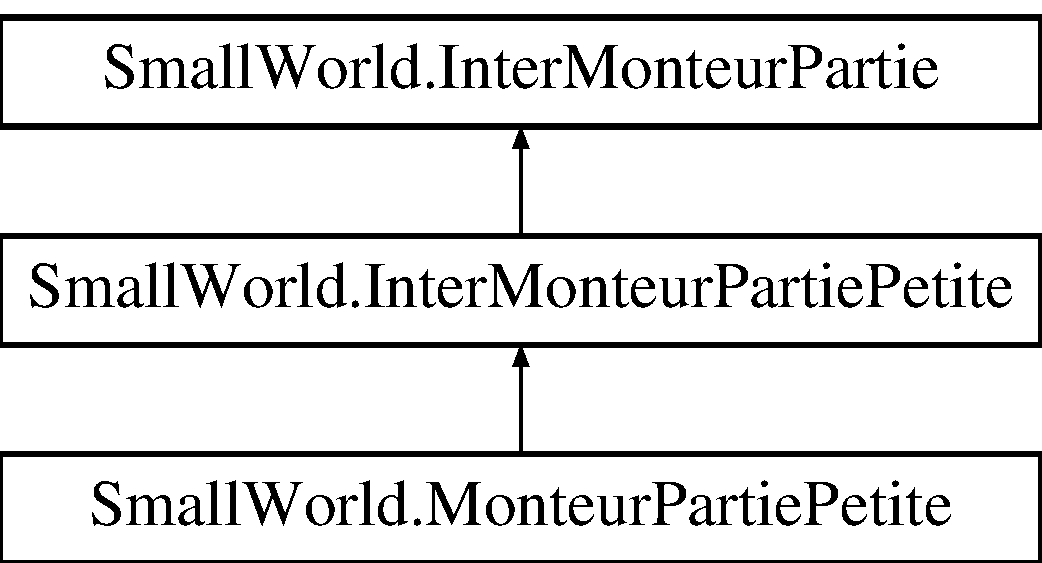
\includegraphics[height=3.000000cm]{interface_small_world_1_1_inter_monteur_partie_petite}
\end{center}
\end{figure}
\subsection*{Public Member Functions}
\begin{DoxyCompactItemize}
\item 
\hypertarget{interface_small_world_1_1_inter_monteur_partie_petite_ac4fae6854406afb775d052ac77c5d0b3}{void {\bfseries ajouter\-Peuple} ()}\label{interface_small_world_1_1_inter_monteur_partie_petite_ac4fae6854406afb775d052ac77c5d0b3}

\end{DoxyCompactItemize}


The documentation for this interface was generated from the following file\-:\begin{DoxyCompactItemize}
\item 
C\-:/\-Users/damienc/\-Documents/\-Git\-Hub/\-Small\-World/\-Visual\-Studio/\-Projet\-P\-O\-O/\hyperlink{_monteur_partie_8cs}{Monteur\-Partie.\-cs}\end{DoxyCompactItemize}

\hypertarget{interface_small_world_1_1_inter_partie}{\section{Small\-World.\-Inter\-Partie Interface Reference}
\label{interface_small_world_1_1_inter_partie}\index{Small\-World.\-Inter\-Partie@{Small\-World.\-Inter\-Partie}}
}


interface pour les partie  


Inheritance diagram for Small\-World.\-Inter\-Partie\-:\begin{figure}[H]
\begin{center}
\leavevmode
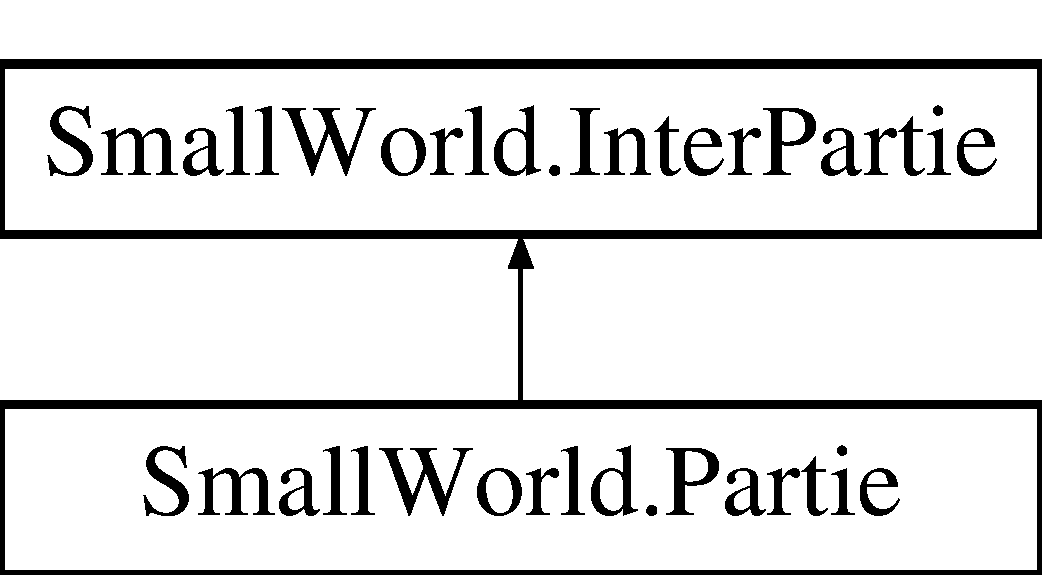
\includegraphics[height=2.000000cm]{interface_small_world_1_1_inter_partie}
\end{center}
\end{figure}
\subsection*{Public Member Functions}
\begin{DoxyCompactItemize}
\item 
List$<$ \hyperlink{class_small_world_1_1_joueur}{Joueur} $>$ \hyperlink{interface_small_world_1_1_inter_partie_a854e4e9df304af71203a90ebea6dd5aa}{vainqueurs} ()
\begin{DoxyCompactList}\small\item\em Rend la liste des joueurs disposant du plus de points. \end{DoxyCompactList}\item 
void \hyperlink{interface_small_world_1_1_inter_partie_a9d379ea16f666ff33913f4c4bb0ac148}{changer\-Joueur} ()
\begin{DoxyCompactList}\small\item\em Change le joueur en cours, quand le joueur précédent a fini son tour. \end{DoxyCompactList}\item 
List$<$ \hyperlink{class_small_world_1_1_unite}{Unite} $>$ \hyperlink{interface_small_world_1_1_inter_partie_aa29e03573a21b6d366bfb8dfb7bd50c3}{selectionner\-Unite} (int x, int y)
\begin{DoxyCompactList}\small\item\em Obtenir l'ensemble des unités du joueur en cours se situant sur la case demandée. \end{DoxyCompactList}\item 
List$<$ \hyperlink{class_small_world_1_1_unite}{Unite} $>$ \hyperlink{interface_small_world_1_1_inter_partie_a3ee997cdbcf1402c3aed3fbad6ff8c56}{selectionner\-Unite\-Adverse} (int x, int y)
\begin{DoxyCompactList}\small\item\em Obtenir l'ensemble des unités des joueurs adverses du joueur en cours se situant sur la case demandée. \end{DoxyCompactList}\item 
bool \hyperlink{interface_small_world_1_1_inter_partie_a1bebb4f8184527d91080a537c759da7b}{peut\-Se\-Deplacer} (\hyperlink{class_small_world_1_1_unite}{Unite} unite, int x, int y)
\begin{DoxyCompactList}\small\item\em Indique si l'unité peut se déposer sur la case(x,y) \end{DoxyCompactList}\item 
int \hyperlink{interface_small_world_1_1_inter_partie_a532da197c321c61ba9c075e00d02bde9}{demander\-Deplacement} (\hyperlink{class_small_world_1_1_unite}{Unite} unite, int x, int y)
\begin{DoxyCompactList}\small\item\em Déplacer, si possible, l'unité sur la case (x,y). En cas d'unités adverses, il y a combat. \end{DoxyCompactList}\item 
void \hyperlink{interface_small_world_1_1_inter_partie_abefef771c059be341130c37dc98876b5}{verifier\-Fin\-Partie} ()
\begin{DoxyCompactList}\small\item\em Vérifier si la partie est finie (les joueurs adverses n'ont plus d'unité) \end{DoxyCompactList}\item 
bool \hyperlink{interface_small_world_1_1_inter_partie_ac1b18e80224dba7e8cb96ae386ed46e3}{enregistrer} ()
\begin{DoxyCompactList}\small\item\em Enregistre une partie. \end{DoxyCompactList}\item 
\hypertarget{interface_small_world_1_1_inter_partie_a04902e267272973c6eec147a87cb2a19}{void {\bfseries enregistrer\-Sous} (string nom\-Fichier)}\label{interface_small_world_1_1_inter_partie_a04902e267272973c6eec147a87cb2a19}

\item 
\hypertarget{interface_small_world_1_1_inter_partie_abb90ffa0496dd58c5333afc32973d28e}{\hyperlink{class_small_world_1_1_partie}{Partie} {\bfseries charger} (string nom\-Fichier)}\label{interface_small_world_1_1_inter_partie_abb90ffa0496dd58c5333afc32973d28e}

\item 
\hypertarget{interface_small_world_1_1_inter_partie_ad80fd5b6fe66be8ac409325e9a15ff33}{void \hyperlink{interface_small_world_1_1_inter_partie_ad80fd5b6fe66be8ac409325e9a15ff33}{restaurer} ()}\label{interface_small_world_1_1_inter_partie_ad80fd5b6fe66be8ac409325e9a15ff33}

\begin{DoxyCompactList}\small\item\em Restaure les unités suite à une désérialisation. \end{DoxyCompactList}\end{DoxyCompactItemize}


\subsection{Detailed Description}
interface pour les partie 

\subsection{Member Function Documentation}
\hypertarget{interface_small_world_1_1_inter_partie_a9d379ea16f666ff33913f4c4bb0ac148}{\index{Small\-World\-::\-Inter\-Partie@{Small\-World\-::\-Inter\-Partie}!changer\-Joueur@{changer\-Joueur}}
\index{changer\-Joueur@{changer\-Joueur}!SmallWorld::InterPartie@{Small\-World\-::\-Inter\-Partie}}
\subsubsection[{changer\-Joueur}]{\setlength{\rightskip}{0pt plus 5cm}Small\-World.\-Inter\-Partie.\-changer\-Joueur (
\begin{DoxyParamCaption}
{}
\end{DoxyParamCaption}
)}}\label{interface_small_world_1_1_inter_partie_a9d379ea16f666ff33913f4c4bb0ac148}


Change le joueur en cours, quand le joueur précédent a fini son tour. 

\begin{DoxyReturn}{Returns}
void 
\end{DoxyReturn}


Implemented in \hyperlink{class_small_world_1_1_partie_a3598df0afeeaa4b0cbf16c5ff8631264}{Small\-World.\-Partie}.

\hypertarget{interface_small_world_1_1_inter_partie_a532da197c321c61ba9c075e00d02bde9}{\index{Small\-World\-::\-Inter\-Partie@{Small\-World\-::\-Inter\-Partie}!demander\-Deplacement@{demander\-Deplacement}}
\index{demander\-Deplacement@{demander\-Deplacement}!SmallWorld::InterPartie@{Small\-World\-::\-Inter\-Partie}}
\subsubsection[{demander\-Deplacement}]{\setlength{\rightskip}{0pt plus 5cm}Small\-World.\-Inter\-Partie.\-demander\-Deplacement (
\begin{DoxyParamCaption}
\item[{{\bf Unite}}]{unite, }
\item[{int}]{x, }
\item[{int}]{y}
\end{DoxyParamCaption}
)}}\label{interface_small_world_1_1_inter_partie_a532da197c321c61ba9c075e00d02bde9}


Déplacer, si possible, l'unité sur la case (x,y). En cas d'unités adverses, il y a combat. 


\begin{DoxyParams}{Parameters}
{\em int} & {\bfseries indice\-Unite} l'indice de l'unité à déplacer, dans le tableau des unités du joueurs en cours \\
\hline
{\em int} & {\bfseries x} l'abscisse de la case destination \\
\hline
{\em int} & {\bfseries y} l'ordonnée de la case destination \\
\hline
\end{DoxyParams}
\begin{DoxyReturn}{Returns}
int, 0 si l'unité ne peut pas se déplacer, 1, si elle se déplace sans combat, 2 s'il y a combat et qu'elle meurt, 3 si combat et déplacement possible, 4 si combat et déplacement non possible 
\end{DoxyReturn}


Implemented in \hyperlink{class_small_world_1_1_partie_a6496b6d4bf683541164126855524897b}{Small\-World.\-Partie}.

\hypertarget{interface_small_world_1_1_inter_partie_ac1b18e80224dba7e8cb96ae386ed46e3}{\index{Small\-World\-::\-Inter\-Partie@{Small\-World\-::\-Inter\-Partie}!enregistrer@{enregistrer}}
\index{enregistrer@{enregistrer}!SmallWorld::InterPartie@{Small\-World\-::\-Inter\-Partie}}
\subsubsection[{enregistrer}]{\setlength{\rightskip}{0pt plus 5cm}Small\-World.\-Inter\-Partie.\-enregistrer (
\begin{DoxyParamCaption}
{}
\end{DoxyParamCaption}
)}}\label{interface_small_world_1_1_inter_partie_ac1b18e80224dba7e8cb96ae386ed46e3}


Enregistre une partie. 

\begin{DoxyReturn}{Returns}
bool, vrai si le nom de fichier est connu, faux sinon 
\end{DoxyReturn}


Implemented in \hyperlink{class_small_world_1_1_partie_a823548e00d1af08c961e0667645d90a9}{Small\-World.\-Partie}.

\hypertarget{interface_small_world_1_1_inter_partie_a1bebb4f8184527d91080a537c759da7b}{\index{Small\-World\-::\-Inter\-Partie@{Small\-World\-::\-Inter\-Partie}!peut\-Se\-Deplacer@{peut\-Se\-Deplacer}}
\index{peut\-Se\-Deplacer@{peut\-Se\-Deplacer}!SmallWorld::InterPartie@{Small\-World\-::\-Inter\-Partie}}
\subsubsection[{peut\-Se\-Deplacer}]{\setlength{\rightskip}{0pt plus 5cm}Small\-World.\-Inter\-Partie.\-peut\-Se\-Deplacer (
\begin{DoxyParamCaption}
\item[{{\bf Unite}}]{unite, }
\item[{int}]{x, }
\item[{int}]{y}
\end{DoxyParamCaption}
)}}\label{interface_small_world_1_1_inter_partie_a1bebb4f8184527d91080a537c759da7b}


Indique si l'unité peut se déposer sur la case(x,y) 


\begin{DoxyParams}{Parameters}
{\em int} & {\bfseries \hyperlink{class_small_world_1_1_unite}{Unite}} l'unité à déplacer \\
\hline
{\em int} & {\bfseries x} l'abscisse de la case destination \\
\hline
{\em int} & {\bfseries y} l'ordonnée de la case destination \\
\hline
\end{DoxyParams}
\begin{DoxyReturn}{Returns}
bool, vrai si le déplacement est possible, faux sinon 
\end{DoxyReturn}


Implemented in \hyperlink{class_small_world_1_1_partie_a8e2f3f866023c8a0e7b817cd6cd42552}{Small\-World.\-Partie}.

\hypertarget{interface_small_world_1_1_inter_partie_aa29e03573a21b6d366bfb8dfb7bd50c3}{\index{Small\-World\-::\-Inter\-Partie@{Small\-World\-::\-Inter\-Partie}!selectionner\-Unite@{selectionner\-Unite}}
\index{selectionner\-Unite@{selectionner\-Unite}!SmallWorld::InterPartie@{Small\-World\-::\-Inter\-Partie}}
\subsubsection[{selectionner\-Unite}]{\setlength{\rightskip}{0pt plus 5cm}Small\-World.\-Inter\-Partie.\-selectionner\-Unite (
\begin{DoxyParamCaption}
\item[{int}]{x, }
\item[{int}]{y}
\end{DoxyParamCaption}
)}}\label{interface_small_world_1_1_inter_partie_aa29e03573a21b6d366bfb8dfb7bd50c3}


Obtenir l'ensemble des unités du joueur en cours se situant sur la case demandée. 


\begin{DoxyParams}{Parameters}
{\em int} & {\bfseries x} l'abcsisse de la case demandée \\
\hline
{\em int} & {\bfseries y} l'ordonnée de la case demandée \\
\hline
\end{DoxyParams}
\begin{DoxyReturn}{Returns}
List$<$\-Unite$>$ la liste des unités présentes sur la cases, pour le joueur courant 
\end{DoxyReturn}


Implemented in \hyperlink{class_small_world_1_1_partie_ab652fc37c8e56f0b1d47d9b12878a04b}{Small\-World.\-Partie}.

\hypertarget{interface_small_world_1_1_inter_partie_a3ee997cdbcf1402c3aed3fbad6ff8c56}{\index{Small\-World\-::\-Inter\-Partie@{Small\-World\-::\-Inter\-Partie}!selectionner\-Unite\-Adverse@{selectionner\-Unite\-Adverse}}
\index{selectionner\-Unite\-Adverse@{selectionner\-Unite\-Adverse}!SmallWorld::InterPartie@{Small\-World\-::\-Inter\-Partie}}
\subsubsection[{selectionner\-Unite\-Adverse}]{\setlength{\rightskip}{0pt plus 5cm}Small\-World.\-Inter\-Partie.\-selectionner\-Unite\-Adverse (
\begin{DoxyParamCaption}
\item[{int}]{x, }
\item[{int}]{y}
\end{DoxyParamCaption}
)}}\label{interface_small_world_1_1_inter_partie_a3ee997cdbcf1402c3aed3fbad6ff8c56}


Obtenir l'ensemble des unités des joueurs adverses du joueur en cours se situant sur la case demandée. 


\begin{DoxyParams}{Parameters}
{\em int} & {\bfseries x} l'abcsisse de la case demandée \\
\hline
{\em int} & {\bfseries y} l'ordonnée de la case demandée \\
\hline
\end{DoxyParams}
\begin{DoxyReturn}{Returns}
List$<$\-Unite$>$ la liste des unités présentes sur la cases, pour les adversaires du joueur courant 
\end{DoxyReturn}


Implemented in \hyperlink{class_small_world_1_1_partie_a78b2a635ab41467c0458172d465bd00a}{Small\-World.\-Partie}.

\hypertarget{interface_small_world_1_1_inter_partie_a854e4e9df304af71203a90ebea6dd5aa}{\index{Small\-World\-::\-Inter\-Partie@{Small\-World\-::\-Inter\-Partie}!vainqueurs@{vainqueurs}}
\index{vainqueurs@{vainqueurs}!SmallWorld::InterPartie@{Small\-World\-::\-Inter\-Partie}}
\subsubsection[{vainqueurs}]{\setlength{\rightskip}{0pt plus 5cm}Small\-World.\-Inter\-Partie.\-vainqueurs (
\begin{DoxyParamCaption}
{}
\end{DoxyParamCaption}
)}}\label{interface_small_world_1_1_inter_partie_a854e4e9df304af71203a90ebea6dd5aa}


Rend la liste des joueurs disposant du plus de points. 

\begin{DoxyReturn}{Returns}
Liste$<$\-Joueur$>$ la liste des gagnants 
\end{DoxyReturn}


Implemented in \hyperlink{class_small_world_1_1_partie_aaf0f50bb8fc7f2841a073f9536579561}{Small\-World.\-Partie}.

\hypertarget{interface_small_world_1_1_inter_partie_abefef771c059be341130c37dc98876b5}{\index{Small\-World\-::\-Inter\-Partie@{Small\-World\-::\-Inter\-Partie}!verifier\-Fin\-Partie@{verifier\-Fin\-Partie}}
\index{verifier\-Fin\-Partie@{verifier\-Fin\-Partie}!SmallWorld::InterPartie@{Small\-World\-::\-Inter\-Partie}}
\subsubsection[{verifier\-Fin\-Partie}]{\setlength{\rightskip}{0pt plus 5cm}Small\-World.\-Inter\-Partie.\-verifier\-Fin\-Partie (
\begin{DoxyParamCaption}
{}
\end{DoxyParamCaption}
)}}\label{interface_small_world_1_1_inter_partie_abefef771c059be341130c37dc98876b5}


Vérifier si la partie est finie (les joueurs adverses n'ont plus d'unité) 

Met la variable Partie\-Finie à vraie si besoin

\begin{DoxyReturn}{Returns}
void 
\end{DoxyReturn}


Implemented in \hyperlink{class_small_world_1_1_partie_a64b2d8fa9405d2a1f588dfa5536bd7a4}{Small\-World.\-Partie}.



The documentation for this interface was generated from the following file\-:\begin{DoxyCompactItemize}
\item 
C\-:/\-Users/damienc/\-Documents/\-Git\-Hub/\-Small\-World/\-Visual\-Studio/\-Projet\-P\-O\-O/\hyperlink{_partie_8cs}{Partie.\-cs}\end{DoxyCompactItemize}

\hypertarget{interface_small_world_1_1_inter_peuple}{\section{Small\-World.\-Inter\-Peuple Interface Reference}
\label{interface_small_world_1_1_inter_peuple}\index{Small\-World.\-Inter\-Peuple@{Small\-World.\-Inter\-Peuple}}
}


interface globale pour les peuples  


Inheritance diagram for Small\-World.\-Inter\-Peuple\-:\begin{figure}[H]
\begin{center}
\leavevmode
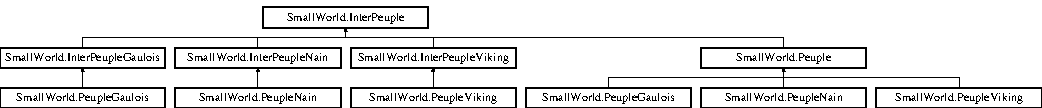
\includegraphics[height=1.450777cm]{interface_small_world_1_1_inter_peuple}
\end{center}
\end{figure}
\subsection*{Public Member Functions}
\begin{DoxyCompactItemize}
\item 
\hyperlink{class_small_world_1_1_unite}{Unite} \hyperlink{interface_small_world_1_1_inter_peuple_affaf908f250e1feb40b90598124dbb56}{creer\-Unite} ()
\begin{DoxyCompactList}\small\item\em créer une unité \end{DoxyCompactList}\end{DoxyCompactItemize}


\subsection{Detailed Description}
interface globale pour les peuples 

\subsection{Member Function Documentation}
\hypertarget{interface_small_world_1_1_inter_peuple_affaf908f250e1feb40b90598124dbb56}{\index{Small\-World\-::\-Inter\-Peuple@{Small\-World\-::\-Inter\-Peuple}!creer\-Unite@{creer\-Unite}}
\index{creer\-Unite@{creer\-Unite}!SmallWorld::InterPeuple@{Small\-World\-::\-Inter\-Peuple}}
\subsubsection[{creer\-Unite}]{\setlength{\rightskip}{0pt plus 5cm}Small\-World.\-Inter\-Peuple.\-creer\-Unite (
\begin{DoxyParamCaption}
{}
\end{DoxyParamCaption}
)}}\label{interface_small_world_1_1_inter_peuple_affaf908f250e1feb40b90598124dbb56}


créer une unité 

\begin{DoxyReturn}{Returns}
l'unité 
\end{DoxyReturn}


Implemented in \hyperlink{class_small_world_1_1_peuple_viking_a28216d67245dc1c8db45b4c9d763923f}{Small\-World.\-Peuple\-Viking}, \hyperlink{class_small_world_1_1_peuple_nain_a31cf5c32229c6f88acf69de84a8c6ebf}{Small\-World.\-Peuple\-Nain}, \hyperlink{class_small_world_1_1_peuple_gaulois_aac9e86d3354a8c4e588a942c705539ee}{Small\-World.\-Peuple\-Gaulois}, and \hyperlink{class_small_world_1_1_peuple_a9d7edd46744bf12c7592b93342835a9b}{Small\-World.\-Peuple}.



The documentation for this interface was generated from the following file\-:\begin{DoxyCompactItemize}
\item 
C\-:/\-Users/damienc/\-Documents/\-Git\-Hub/\-Small\-World/\-Visual\-Studio/\-Projet\-P\-O\-O/\hyperlink{_peuple_8cs}{Peuple.\-cs}\end{DoxyCompactItemize}

\hypertarget{interface_small_world_1_1_inter_peuple_gaulois}{\section{Small\-World.\-Inter\-Peuple\-Gaulois Interface Reference}
\label{interface_small_world_1_1_inter_peuple_gaulois}\index{Small\-World.\-Inter\-Peuple\-Gaulois@{Small\-World.\-Inter\-Peuple\-Gaulois}}
}
Inheritance diagram for Small\-World.\-Inter\-Peuple\-Gaulois\-:\begin{figure}[H]
\begin{center}
\leavevmode
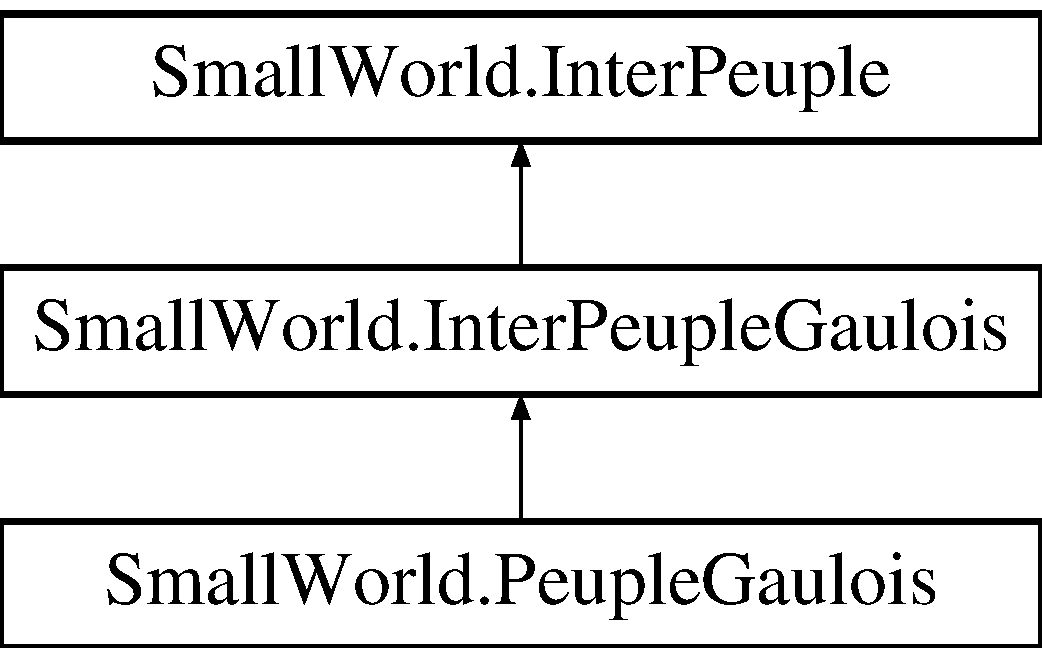
\includegraphics[height=3.000000cm]{interface_small_world_1_1_inter_peuple_gaulois}
\end{center}
\end{figure}
\subsection*{Additional Inherited Members}


The documentation for this interface was generated from the following file\-:\begin{DoxyCompactItemize}
\item 
C\-:/\-Users/damienc/\-Documents/\-Git\-Hub/\-Small\-World/\-Visual\-Studio/\-Projet\-P\-O\-O/Peuple\-Gaulois.\-cs\end{DoxyCompactItemize}

\hypertarget{interface_small_world_1_1_inter_peuple_nain}{\section{Small\-World.\-Inter\-Peuple\-Nain Interface Reference}
\label{interface_small_world_1_1_inter_peuple_nain}\index{Small\-World.\-Inter\-Peuple\-Nain@{Small\-World.\-Inter\-Peuple\-Nain}}
}
Inheritance diagram for Small\-World.\-Inter\-Peuple\-Nain\-:\begin{figure}[H]
\begin{center}
\leavevmode
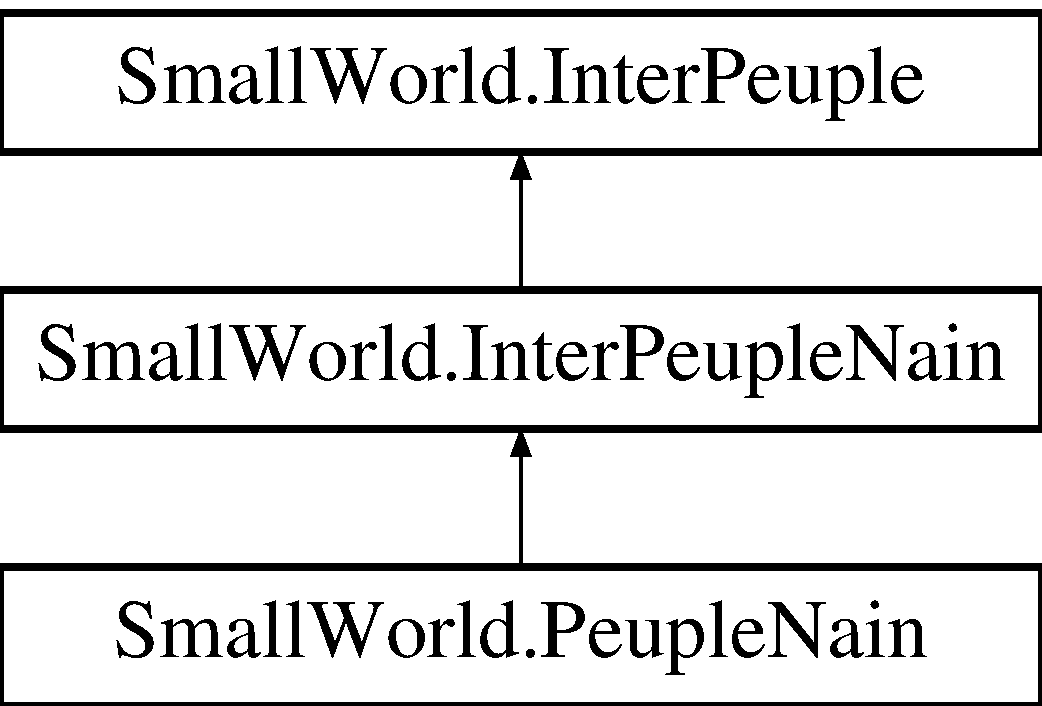
\includegraphics[height=3.000000cm]{interface_small_world_1_1_inter_peuple_nain}
\end{center}
\end{figure}
\subsection*{Additional Inherited Members}


The documentation for this interface was generated from the following file\-:\begin{DoxyCompactItemize}
\item 
C\-:/\-Users/damienc/\-Documents/\-Git\-Hub/\-Small\-World/\-Visual\-Studio/\-Projet\-P\-O\-O/Peuple\-Nain.\-cs\end{DoxyCompactItemize}

\hypertarget{interface_small_world_1_1_inter_peuple_viking}{\section{Small\-World.\-Inter\-Peuple\-Viking Interface Reference}
\label{interface_small_world_1_1_inter_peuple_viking}\index{Small\-World.\-Inter\-Peuple\-Viking@{Small\-World.\-Inter\-Peuple\-Viking}}
}
Inheritance diagram for Small\-World.\-Inter\-Peuple\-Viking\-:\begin{figure}[H]
\begin{center}
\leavevmode
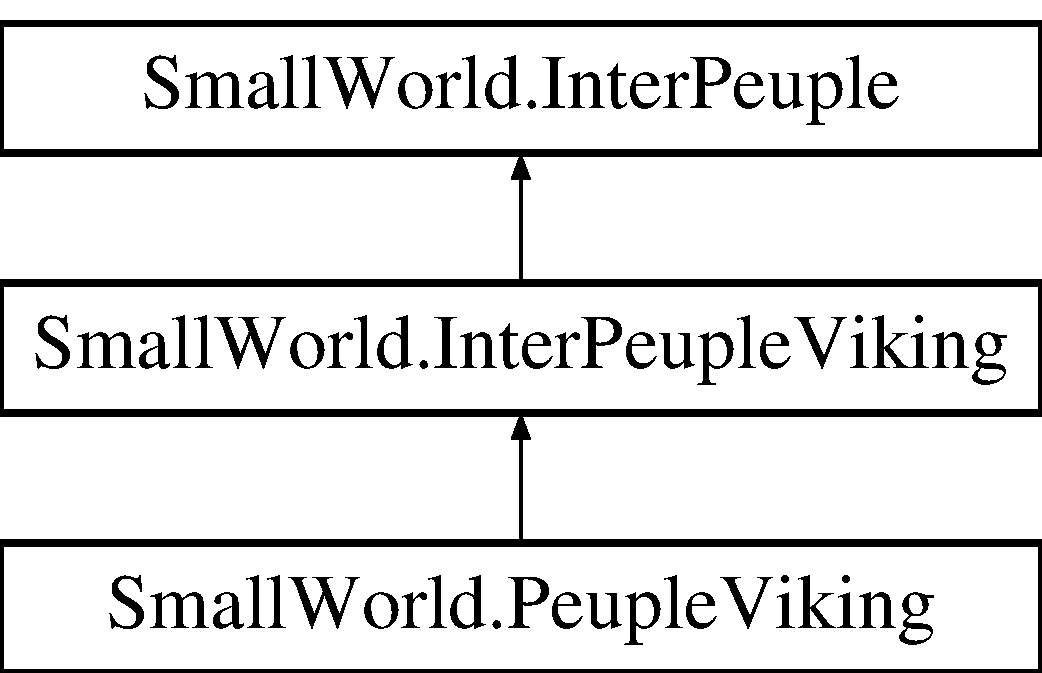
\includegraphics[height=3.000000cm]{interface_small_world_1_1_inter_peuple_viking}
\end{center}
\end{figure}
\subsection*{Additional Inherited Members}


The documentation for this interface was generated from the following file\-:\begin{DoxyCompactItemize}
\item 
C\-:/\-Users/damienc/\-Documents/\-Git\-Hub/\-Small\-World/\-Visual\-Studio/\-Projet\-P\-O\-O/Peuple\-Viking.\-cs\end{DoxyCompactItemize}

\hypertarget{interface_small_world_1_1_inter_plaine}{\section{Small\-World.\-Inter\-Plaine Interface Reference}
\label{interface_small_world_1_1_inter_plaine}\index{Small\-World.\-Inter\-Plaine@{Small\-World.\-Inter\-Plaine}}
}


Interface pour \hyperlink{class_small_world_1_1_case}{Case} de type plaine.  


Inheritance diagram for Small\-World.\-Inter\-Plaine\-:\begin{figure}[H]
\begin{center}
\leavevmode
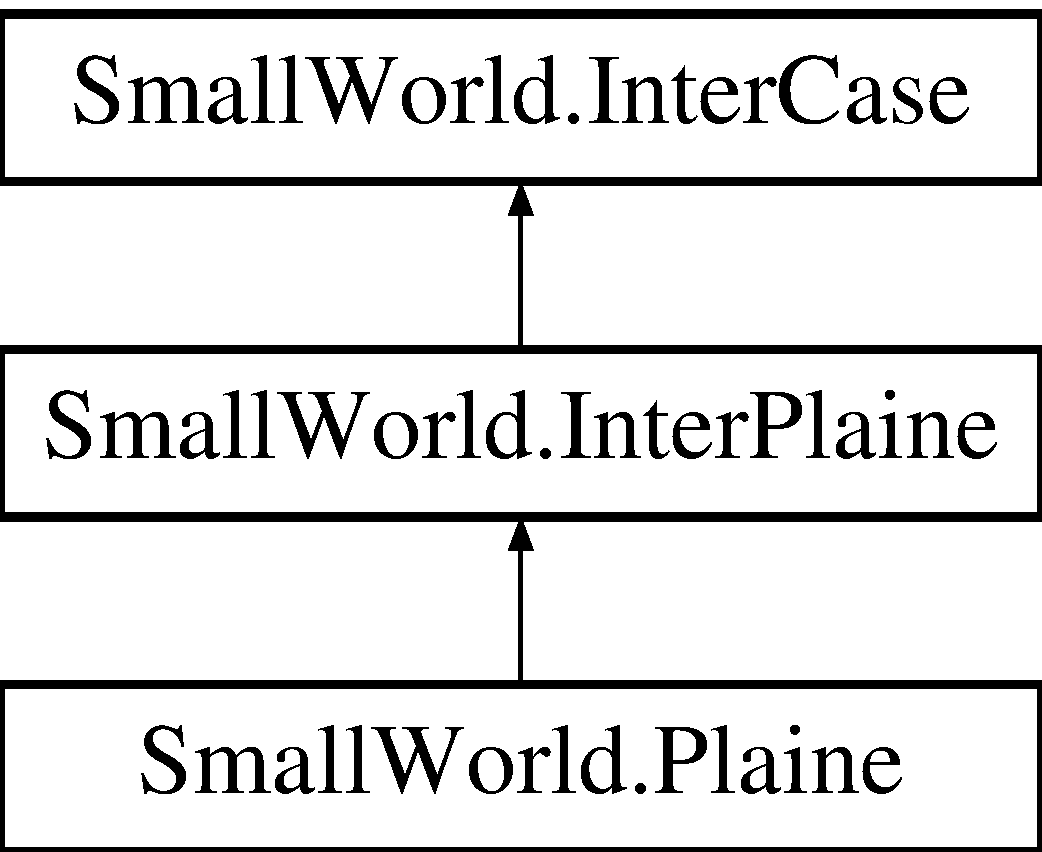
\includegraphics[height=3.000000cm]{interface_small_world_1_1_inter_plaine}
\end{center}
\end{figure}


\subsection{Detailed Description}
Interface pour \hyperlink{class_small_world_1_1_case}{Case} de type plaine. 

The documentation for this interface was generated from the following file\-:\begin{DoxyCompactItemize}
\item 
C\-:/\-Users/damienc/\-Documents/\-Git\-Hub/\-Small\-World/\-Visual\-Studio/\-Projet\-P\-O\-O/\hyperlink{_case_8cs}{Case.\-cs}\end{DoxyCompactItemize}

\hypertarget{interface_small_world_1_1_inter_strategie_carte}{\section{Small\-World.\-Inter\-Strategie\-Carte Interface Reference}
\label{interface_small_world_1_1_inter_strategie_carte}\index{Small\-World.\-Inter\-Strategie\-Carte@{Small\-World.\-Inter\-Strategie\-Carte}}
}


interface globale pour la stratégie  


Inheritance diagram for Small\-World.\-Inter\-Strategie\-Carte\-:\begin{figure}[H]
\begin{center}
\leavevmode
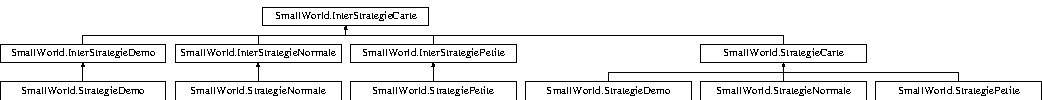
\includegraphics[height=1.339713cm]{interface_small_world_1_1_inter_strategie_carte}
\end{center}
\end{figure}
\subsection*{Public Member Functions}
\begin{DoxyCompactItemize}
\item 
\hypertarget{interface_small_world_1_1_inter_strategie_carte_aef481b6ecc1f7976bd197147709998b0}{List$<$ List$<$ \hyperlink{class_small_world_1_1_case}{Case} $>$ $>$ \hyperlink{interface_small_world_1_1_inter_strategie_carte_aef481b6ecc1f7976bd197147709998b0}{construire} ()}\label{interface_small_world_1_1_inter_strategie_carte_aef481b6ecc1f7976bd197147709998b0}

\begin{DoxyCompactList}\small\item\em Construit une nouvelle \hyperlink{class_small_world_1_1_carte}{Carte}. \end{DoxyCompactList}\end{DoxyCompactItemize}


\subsection{Detailed Description}
interface globale pour la stratégie 

The documentation for this interface was generated from the following file\-:\begin{DoxyCompactItemize}
\item 
C\-:/\-Users/damienc/\-Documents/\-Git\-Hub/\-Small\-World/\-Visual\-Studio/\-Projet\-P\-O\-O/\hyperlink{_strategie_8cs}{Strategie.\-cs}\end{DoxyCompactItemize}

\hypertarget{interface_small_world_1_1_inter_strategie_demo}{\section{Small\-World.\-Inter\-Strategie\-Demo Interface Reference}
\label{interface_small_world_1_1_inter_strategie_demo}\index{Small\-World.\-Inter\-Strategie\-Demo@{Small\-World.\-Inter\-Strategie\-Demo}}
}
Inheritance diagram for Small\-World.\-Inter\-Strategie\-Demo\-:\begin{figure}[H]
\begin{center}
\leavevmode
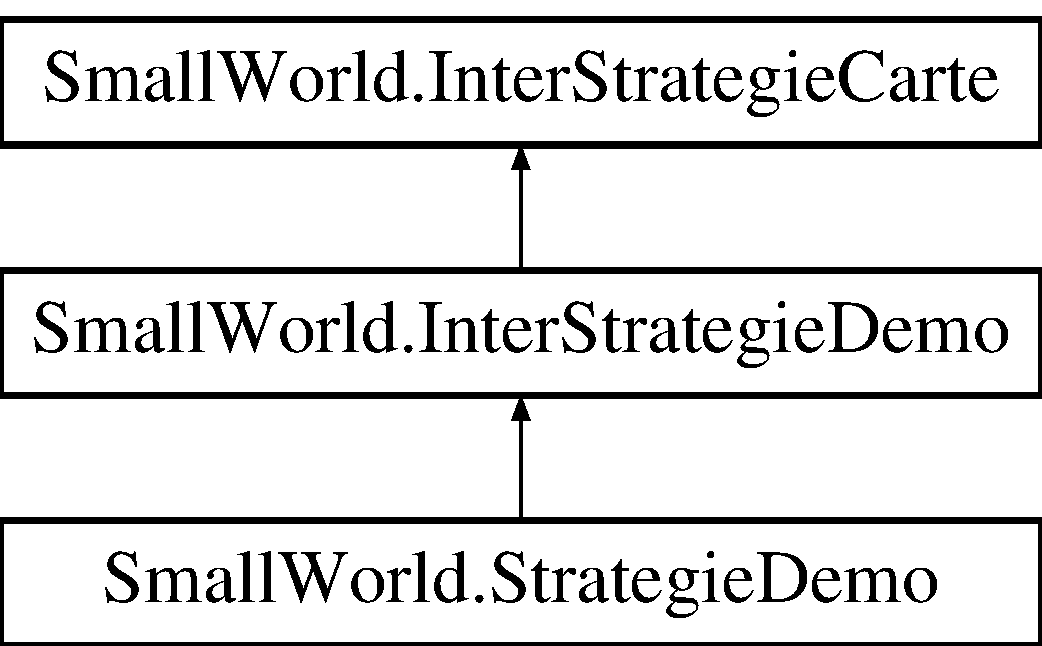
\includegraphics[height=3.000000cm]{interface_small_world_1_1_inter_strategie_demo}
\end{center}
\end{figure}
\subsection*{Public Member Functions}
\begin{DoxyCompactItemize}
\item 
new void \hyperlink{interface_small_world_1_1_inter_strategie_demo_a302a516e2be5370c90ecd6e73b100f73}{construire} ()
\end{DoxyCompactItemize}


\subsection{Member Function Documentation}
\hypertarget{interface_small_world_1_1_inter_strategie_demo_a302a516e2be5370c90ecd6e73b100f73}{\index{Small\-World\-::\-Inter\-Strategie\-Demo@{Small\-World\-::\-Inter\-Strategie\-Demo}!construire@{construire}}
\index{construire@{construire}!SmallWorld::InterStrategieDemo@{Small\-World\-::\-Inter\-Strategie\-Demo}}
\subsubsection[{construire}]{\setlength{\rightskip}{0pt plus 5cm}new void Small\-World.\-Inter\-Strategie\-Demo.\-construire (
\begin{DoxyParamCaption}
{}
\end{DoxyParamCaption}
)}}\label{interface_small_world_1_1_inter_strategie_demo_a302a516e2be5370c90ecd6e73b100f73}


Implements \hyperlink{interface_small_world_1_1_inter_strategie_carte_aa3f0d1267ad71756dc3b134d13733085}{Small\-World.\-Inter\-Strategie\-Carte}.



Implemented in \hyperlink{class_small_world_1_1_strategie_demo_afc2d6c69d19a33fa894c3193d7244200}{Small\-World.\-Strategie\-Demo}.



The documentation for this interface was generated from the following file\-:\begin{DoxyCompactItemize}
\item 
C\-:/\-Users/damienc/\-Documents/\-Git\-Hub/\-Small\-World/\-Visual\-Studio/\-Projet\-P\-O\-O/Strategie.\-cs\end{DoxyCompactItemize}

\hypertarget{interface_small_world_1_1_inter_strategie_normale}{\section{Small\-World.\-Inter\-Strategie\-Normale Interface Reference}
\label{interface_small_world_1_1_inter_strategie_normale}\index{Small\-World.\-Inter\-Strategie\-Normale@{Small\-World.\-Inter\-Strategie\-Normale}}
}
Inheritance diagram for Small\-World.\-Inter\-Strategie\-Normale\-:\begin{figure}[H]
\begin{center}
\leavevmode
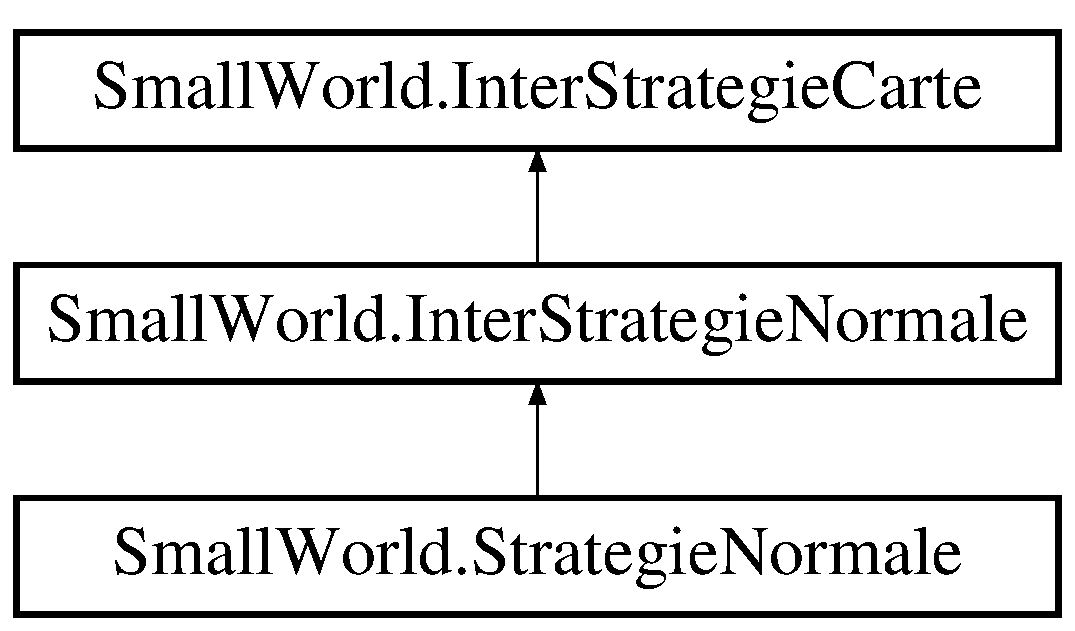
\includegraphics[height=3.000000cm]{interface_small_world_1_1_inter_strategie_normale}
\end{center}
\end{figure}
\subsection*{Public Member Functions}
\begin{DoxyCompactItemize}
\item 
void \hyperlink{interface_small_world_1_1_inter_strategie_normale_a6488d973a40d587a3357b6e690104258}{construire} ()
\end{DoxyCompactItemize}


\subsection{Member Function Documentation}
\hypertarget{interface_small_world_1_1_inter_strategie_normale_a6488d973a40d587a3357b6e690104258}{\index{Small\-World\-::\-Inter\-Strategie\-Normale@{Small\-World\-::\-Inter\-Strategie\-Normale}!construire@{construire}}
\index{construire@{construire}!SmallWorld::InterStrategieNormale@{Small\-World\-::\-Inter\-Strategie\-Normale}}
\subsubsection[{construire}]{\setlength{\rightskip}{0pt plus 5cm}void Small\-World.\-Inter\-Strategie\-Normale.\-construire (
\begin{DoxyParamCaption}
{}
\end{DoxyParamCaption}
)}}\label{interface_small_world_1_1_inter_strategie_normale_a6488d973a40d587a3357b6e690104258}


Implements \hyperlink{interface_small_world_1_1_inter_strategie_carte_aa3f0d1267ad71756dc3b134d13733085}{Small\-World.\-Inter\-Strategie\-Carte}.



Implemented in \hyperlink{class_small_world_1_1_strategie_normale_a7f3732b81d0b4b1e11dae277d6db219c}{Small\-World.\-Strategie\-Normale}.



The documentation for this interface was generated from the following file\-:\begin{DoxyCompactItemize}
\item 
C\-:/\-Users/damienc/\-Documents/\-Git\-Hub/\-Small\-World/\-Visual\-Studio/\-Projet\-P\-O\-O/Normale.\-cs\end{DoxyCompactItemize}

\hypertarget{interface_small_world_1_1_inter_strategie_petite}{\section{Small\-World.\-Inter\-Strategie\-Petite Interface Reference}
\label{interface_small_world_1_1_inter_strategie_petite}\index{Small\-World.\-Inter\-Strategie\-Petite@{Small\-World.\-Inter\-Strategie\-Petite}}
}


interface pour une stratégie petite  


Inheritance diagram for Small\-World.\-Inter\-Strategie\-Petite\-:\begin{figure}[H]
\begin{center}
\leavevmode
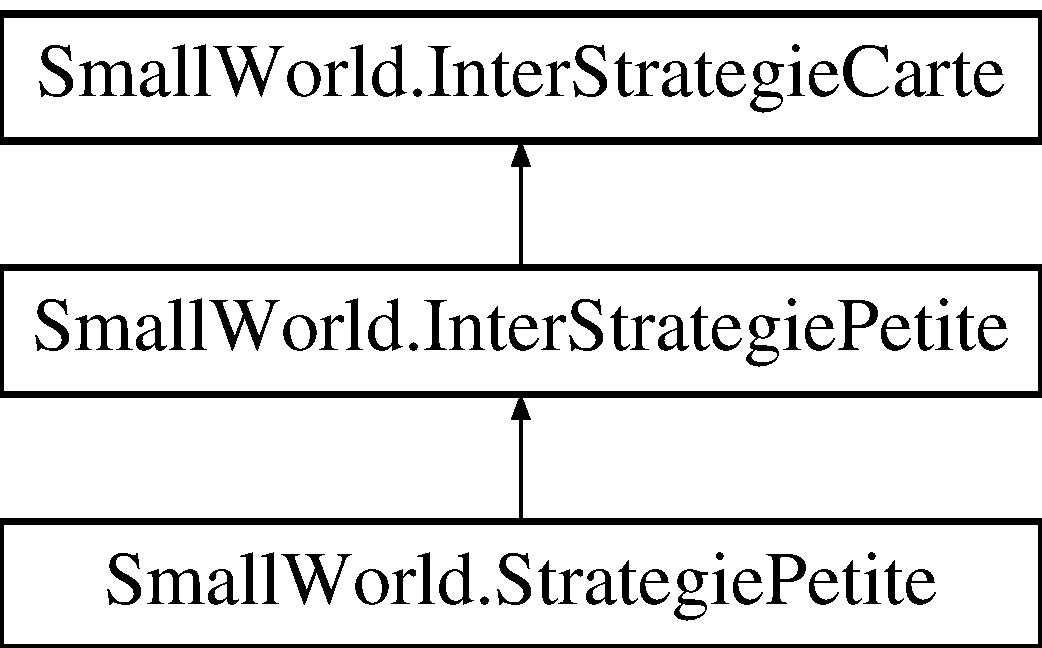
\includegraphics[height=3.000000cm]{interface_small_world_1_1_inter_strategie_petite}
\end{center}
\end{figure}
\subsection*{Public Member Functions}
\begin{DoxyCompactItemize}
\item 
new List$<$ List$<$ \hyperlink{class_small_world_1_1_case}{Case} $>$ $>$ \hyperlink{interface_small_world_1_1_inter_strategie_petite_adb06e8f32bcbb5d9f491f86f5ea34a0e}{construire} ()
\begin{DoxyCompactList}\small\item\em contruit une carte de taille petite \end{DoxyCompactList}\end{DoxyCompactItemize}


\subsection{Detailed Description}
interface pour une stratégie petite 

\subsection{Member Function Documentation}
\hypertarget{interface_small_world_1_1_inter_strategie_petite_adb06e8f32bcbb5d9f491f86f5ea34a0e}{\index{Small\-World\-::\-Inter\-Strategie\-Petite@{Small\-World\-::\-Inter\-Strategie\-Petite}!construire@{construire}}
\index{construire@{construire}!SmallWorld::InterStrategiePetite@{Small\-World\-::\-Inter\-Strategie\-Petite}}
\subsubsection[{construire}]{\setlength{\rightskip}{0pt plus 5cm}Small\-World.\-Inter\-Strategie\-Petite.\-construire (
\begin{DoxyParamCaption}
{}
\end{DoxyParamCaption}
)}}\label{interface_small_world_1_1_inter_strategie_petite_adb06e8f32bcbb5d9f491f86f5ea34a0e}


contruit une carte de taille petite 

\begin{DoxyReturn}{Returns}
la carte demandée 
\end{DoxyReturn}


Implements \hyperlink{interface_small_world_1_1_inter_strategie_carte_aef481b6ecc1f7976bd197147709998b0}{Small\-World.\-Inter\-Strategie\-Carte}.



The documentation for this interface was generated from the following file\-:\begin{DoxyCompactItemize}
\item 
C\-:/\-Users/damienc/\-Documents/\-Git\-Hub/\-Small\-World/\-Visual\-Studio/\-Projet\-P\-O\-O/\hyperlink{_strategie_8cs}{Strategie.\-cs}\end{DoxyCompactItemize}

\hypertarget{interface_small_world_1_1_inter_unite}{\section{Small\-World.\-Inter\-Unite Interface Reference}
\label{interface_small_world_1_1_inter_unite}\index{Small\-World.\-Inter\-Unite@{Small\-World.\-Inter\-Unite}}
}


interface pour les unités  


Inheritance diagram for Small\-World.\-Inter\-Unite\-:\begin{figure}[H]
\begin{center}
\leavevmode
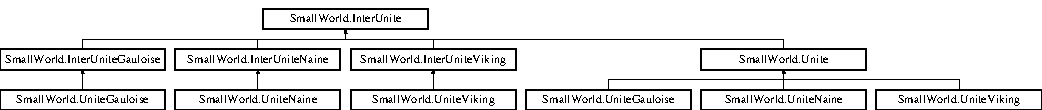
\includegraphics[height=1.481482cm]{interface_small_world_1_1_inter_unite}
\end{center}
\end{figure}
\subsection*{Public Member Functions}
\begin{DoxyCompactItemize}
\item 
\hypertarget{interface_small_world_1_1_inter_unite_a729d769c596c3df5e0f8d1d460de4d5e}{void \hyperlink{interface_small_world_1_1_inter_unite_a729d769c596c3df5e0f8d1d460de4d5e}{calcul\-Point\-Victoire} ()}\label{interface_small_world_1_1_inter_unite_a729d769c596c3df5e0f8d1d460de4d5e}

\begin{DoxyCompactList}\small\item\em Met à jour les points de victoire du joueur. \end{DoxyCompactList}\item 
void \hyperlink{interface_small_world_1_1_inter_unite_a9bce76356ba4531ed90ca35cc659af5f}{attaquer} (\hyperlink{class_small_world_1_1_unite}{Unite} unite\-Adverse, int nb\-Round\-Combat)
\begin{DoxyCompactList}\small\item\em attaquer une unité adverse, sachant le nombre de rounds \end{DoxyCompactList}\item 
bool \hyperlink{interface_small_world_1_1_inter_unite_aac3a60f40b315d1f3c1299e906ebb384}{se\-Deplacer} (int x, int y)
\begin{DoxyCompactList}\small\item\em se déplacer sur une case \end{DoxyCompactList}\item 
bool \hyperlink{interface_small_world_1_1_inter_unite_a28644be4f50b3370dd276a2aa274413f}{peut\-Se\-Deplacer} (int x, int y)
\begin{DoxyCompactList}\small\item\em Indique si l'unité peut se déplacer sur une case. \end{DoxyCompactList}\item 
void \hyperlink{interface_small_world_1_1_inter_unite_aaf0cbd85facc23d866aac19dad7f3e66}{calculer\-Deplacement} ()
\begin{DoxyCompactList}\small\item\em calculer les déplacements possibles \end{DoxyCompactList}\item 
\hypertarget{interface_small_world_1_1_inter_unite_ada8a39324c90c82eb25a978fa81b43f1}{void \hyperlink{interface_small_world_1_1_inter_unite_ada8a39324c90c82eb25a978fa81b43f1}{passer\-Son\-Tour} ()}\label{interface_small_world_1_1_inter_unite_ada8a39324c90c82eb25a978fa81b43f1}

\begin{DoxyCompactList}\small\item\em l'unité passe son tour \end{DoxyCompactList}\item 
\hypertarget{interface_small_world_1_1_inter_unite_a106ab0a27d4a228dbcf18c0b26f680b3}{void \hyperlink{interface_small_world_1_1_inter_unite_a106ab0a27d4a228dbcf18c0b26f680b3}{perdre\-Vie} ()}\label{interface_small_world_1_1_inter_unite_a106ab0a27d4a228dbcf18c0b26f680b3}

\begin{DoxyCompactList}\small\item\em l'unité perd une vie \end{DoxyCompactList}\item 
\hypertarget{interface_small_world_1_1_inter_unite_a2c19b9dc612ee1ec4716f9993b78908d}{void \hyperlink{interface_small_world_1_1_inter_unite_a2c19b9dc612ee1ec4716f9993b78908d}{nouveau\-Tour} ()}\label{interface_small_world_1_1_inter_unite_a2c19b9dc612ee1ec4716f9993b78908d}

\begin{DoxyCompactList}\small\item\em Les attributs de l'unité sont mis à jour pour le nouveau tour. \end{DoxyCompactList}\item 
void \hyperlink{interface_small_world_1_1_inter_unite_a554b5ca4373b37e6e5ad29f3a3a381dc}{restaurer} (int $\ast$carte)
\begin{DoxyCompactList}\small\item\em Restaure l'unité suite à une désérialisation. \end{DoxyCompactList}\item 
List$<$ \hyperlink{class_small_world_1_1_coordonnees}{Coordonnees} $>$ \hyperlink{interface_small_world_1_1_inter_unite_a1c5011629159c486f68c015dc940406e}{suggerer\-Case\-Non\-Possible} ()
\begin{DoxyCompactList}\small\item\em Suggère les cases de déplacement impossible pour une unité \end{DoxyCompactList}\item 
List$<$ \hyperlink{class_small_world_1_1_coordonnees}{Coordonnees} $>$ \hyperlink{interface_small_world_1_1_inter_unite_ac0016b4cfb075557c4e2bcc6a1b1876e}{suggerer\-Case\-Optimale} ()
\begin{DoxyCompactList}\small\item\em Suggère les cases de déplacement pour une unité qui sont optimales. \end{DoxyCompactList}\end{DoxyCompactItemize}


\subsection{Detailed Description}
interface pour les unités 

\subsection{Member Function Documentation}
\hypertarget{interface_small_world_1_1_inter_unite_a9bce76356ba4531ed90ca35cc659af5f}{\index{Small\-World\-::\-Inter\-Unite@{Small\-World\-::\-Inter\-Unite}!attaquer@{attaquer}}
\index{attaquer@{attaquer}!SmallWorld::InterUnite@{Small\-World\-::\-Inter\-Unite}}
\subsubsection[{attaquer}]{\setlength{\rightskip}{0pt plus 5cm}Small\-World.\-Inter\-Unite.\-attaquer (
\begin{DoxyParamCaption}
\item[{{\bf Unite}}]{unite\-Adverse, }
\item[{int}]{nb\-Round\-Combat}
\end{DoxyParamCaption}
)}}\label{interface_small_world_1_1_inter_unite_a9bce76356ba4531ed90ca35cc659af5f}


attaquer une unité adverse, sachant le nombre de rounds 


\begin{DoxyParams}{Parameters}
{\em \hyperlink{class_small_world_1_1_unite}{Unite}} & {\bfseries unite\-Adverse} l'unité à combattre \\
\hline
{\em int} & {\bfseries nb\-Round\-Combat} le nombre de round \\
\hline
\end{DoxyParams}


Implemented in \hyperlink{class_small_world_1_1_unite_af370920ab6c2b9478f0c12d7f1d22638}{Small\-World.\-Unite}.

\hypertarget{interface_small_world_1_1_inter_unite_aaf0cbd85facc23d866aac19dad7f3e66}{\index{Small\-World\-::\-Inter\-Unite@{Small\-World\-::\-Inter\-Unite}!calculer\-Deplacement@{calculer\-Deplacement}}
\index{calculer\-Deplacement@{calculer\-Deplacement}!SmallWorld::InterUnite@{Small\-World\-::\-Inter\-Unite}}
\subsubsection[{calculer\-Deplacement}]{\setlength{\rightskip}{0pt plus 5cm}Small\-World.\-Inter\-Unite.\-calculer\-Deplacement (
\begin{DoxyParamCaption}
{}
\end{DoxyParamCaption}
)}}\label{interface_small_world_1_1_inter_unite_aaf0cbd85facc23d866aac19dad7f3e66}


calculer les déplacements possibles 

\begin{DoxyReturn}{Returns}
void 
\end{DoxyReturn}


Implemented in \hyperlink{class_small_world_1_1_unite_viking_a7df92edec9b221dc96be2cf60d19f06f}{Small\-World.\-Unite\-Viking}, \hyperlink{class_small_world_1_1_unite_naine_a487e42750e74fbf551d1e55b48101c72}{Small\-World.\-Unite\-Naine}, \hyperlink{class_small_world_1_1_unite_gauloise_a2fce92f8a4957a46efae89b63277b073}{Small\-World.\-Unite\-Gauloise}, and \hyperlink{class_small_world_1_1_unite_a88ea1d2d5962c08ffc15422a2f2c7bbf}{Small\-World.\-Unite}.

\hypertarget{interface_small_world_1_1_inter_unite_a28644be4f50b3370dd276a2aa274413f}{\index{Small\-World\-::\-Inter\-Unite@{Small\-World\-::\-Inter\-Unite}!peut\-Se\-Deplacer@{peut\-Se\-Deplacer}}
\index{peut\-Se\-Deplacer@{peut\-Se\-Deplacer}!SmallWorld::InterUnite@{Small\-World\-::\-Inter\-Unite}}
\subsubsection[{peut\-Se\-Deplacer}]{\setlength{\rightskip}{0pt plus 5cm}Small\-World.\-Inter\-Unite.\-peut\-Se\-Deplacer (
\begin{DoxyParamCaption}
\item[{int}]{x, }
\item[{int}]{y}
\end{DoxyParamCaption}
)}}\label{interface_small_world_1_1_inter_unite_a28644be4f50b3370dd276a2aa274413f}


Indique si l'unité peut se déplacer sur une case. 


\begin{DoxyParams}{Parameters}
{\em int} & {\bfseries x} l'abscisse demandée \\
\hline
{\em int} & {\bfseries y} l'ordonnée demandée \\
\hline
\end{DoxyParams}
\begin{DoxyReturn}{Returns}
bool vrai si l'unité peut se déplacer, faux sinon 
\end{DoxyReturn}


Implemented in \hyperlink{class_small_world_1_1_unite_a26f648e9ca7776ade3e8c335644ed8f1}{Small\-World.\-Unite}.

\hypertarget{interface_small_world_1_1_inter_unite_a554b5ca4373b37e6e5ad29f3a3a381dc}{\index{Small\-World\-::\-Inter\-Unite@{Small\-World\-::\-Inter\-Unite}!restaurer@{restaurer}}
\index{restaurer@{restaurer}!SmallWorld::InterUnite@{Small\-World\-::\-Inter\-Unite}}
\subsubsection[{restaurer}]{\setlength{\rightskip}{0pt plus 5cm}Small\-World.\-Inter\-Unite.\-restaurer (
\begin{DoxyParamCaption}
\item[{int $\ast$}]{carte}
\end{DoxyParamCaption}
)}}\label{interface_small_world_1_1_inter_unite_a554b5ca4373b37e6e5ad29f3a3a381dc}


Restaure l'unité suite à une désérialisation. 

\begin{DoxyReturn}{Returns}
void 
\end{DoxyReturn}


Implemented in \hyperlink{class_small_world_1_1_unite_a6b703c7f442f922c6742f17d96bd2bb3}{Small\-World.\-Unite}.

\hypertarget{interface_small_world_1_1_inter_unite_aac3a60f40b315d1f3c1299e906ebb384}{\index{Small\-World\-::\-Inter\-Unite@{Small\-World\-::\-Inter\-Unite}!se\-Deplacer@{se\-Deplacer}}
\index{se\-Deplacer@{se\-Deplacer}!SmallWorld::InterUnite@{Small\-World\-::\-Inter\-Unite}}
\subsubsection[{se\-Deplacer}]{\setlength{\rightskip}{0pt plus 5cm}Small\-World.\-Inter\-Unite.\-se\-Deplacer (
\begin{DoxyParamCaption}
\item[{int}]{x, }
\item[{int}]{y}
\end{DoxyParamCaption}
)}}\label{interface_small_world_1_1_inter_unite_aac3a60f40b315d1f3c1299e906ebb384}


se déplacer sur une case 


\begin{DoxyParams}{Parameters}
{\em int} & {\bfseries x} l'abscisse demandée \\
\hline
{\em int} & {\bfseries y} l'ordinnée demandée \\
\hline
\end{DoxyParams}
\begin{DoxyReturn}{Returns}
void 
\end{DoxyReturn}


Implemented in \hyperlink{class_small_world_1_1_unite_abc3a49225b122d3dc3579883d433d300}{Small\-World.\-Unite}.

\hypertarget{interface_small_world_1_1_inter_unite_a1c5011629159c486f68c015dc940406e}{\index{Small\-World\-::\-Inter\-Unite@{Small\-World\-::\-Inter\-Unite}!suggerer\-Case\-Non\-Possible@{suggerer\-Case\-Non\-Possible}}
\index{suggerer\-Case\-Non\-Possible@{suggerer\-Case\-Non\-Possible}!SmallWorld::InterUnite@{Small\-World\-::\-Inter\-Unite}}
\subsubsection[{suggerer\-Case\-Non\-Possible}]{\setlength{\rightskip}{0pt plus 5cm}Small\-World.\-Inter\-Unite.\-suggerer\-Case\-Non\-Possible (
\begin{DoxyParamCaption}
{}
\end{DoxyParamCaption}
)}}\label{interface_small_world_1_1_inter_unite_a1c5011629159c486f68c015dc940406e}


Suggère les cases de déplacement impossible pour une unité 

\begin{DoxyReturn}{Returns}
List$<$\-Coordonnee$>$ la liste des coordonnées impossibles 
\end{DoxyReturn}


Implemented in \hyperlink{class_small_world_1_1_unite_a79b7bc972bf0b76647be702cf94965fc}{Small\-World.\-Unite}.

\hypertarget{interface_small_world_1_1_inter_unite_ac0016b4cfb075557c4e2bcc6a1b1876e}{\index{Small\-World\-::\-Inter\-Unite@{Small\-World\-::\-Inter\-Unite}!suggerer\-Case\-Optimale@{suggerer\-Case\-Optimale}}
\index{suggerer\-Case\-Optimale@{suggerer\-Case\-Optimale}!SmallWorld::InterUnite@{Small\-World\-::\-Inter\-Unite}}
\subsubsection[{suggerer\-Case\-Optimale}]{\setlength{\rightskip}{0pt plus 5cm}Small\-World.\-Inter\-Unite.\-suggerer\-Case\-Optimale (
\begin{DoxyParamCaption}
{}
\end{DoxyParamCaption}
)}}\label{interface_small_world_1_1_inter_unite_ac0016b4cfb075557c4e2bcc6a1b1876e}


Suggère les cases de déplacement pour une unité qui sont optimales. 

\begin{DoxyReturn}{Returns}
List$<$\-Coordonnee$>$ la liste des coordonnées possibles 
\end{DoxyReturn}


Implemented in \hyperlink{class_small_world_1_1_unite_a2da8fe0e076dbfccf553b6ecb6c9fc04}{Small\-World.\-Unite}.



The documentation for this interface was generated from the following file\-:\begin{DoxyCompactItemize}
\item 
C\-:/\-Users/damienc/\-Documents/\-Git\-Hub/\-Small\-World/\-Visual\-Studio/\-Projet\-P\-O\-O/\hyperlink{_unite_8cs}{Unite.\-cs}\end{DoxyCompactItemize}

\hypertarget{interface_small_world_1_1_inter_unite_gauloise}{\section{Small\-World.\-Inter\-Unite\-Gauloise Interface Reference}
\label{interface_small_world_1_1_inter_unite_gauloise}\index{Small\-World.\-Inter\-Unite\-Gauloise@{Small\-World.\-Inter\-Unite\-Gauloise}}
}


Interface pour les unités gauloises.  


Inheritance diagram for Small\-World.\-Inter\-Unite\-Gauloise\-:\begin{figure}[H]
\begin{center}
\leavevmode
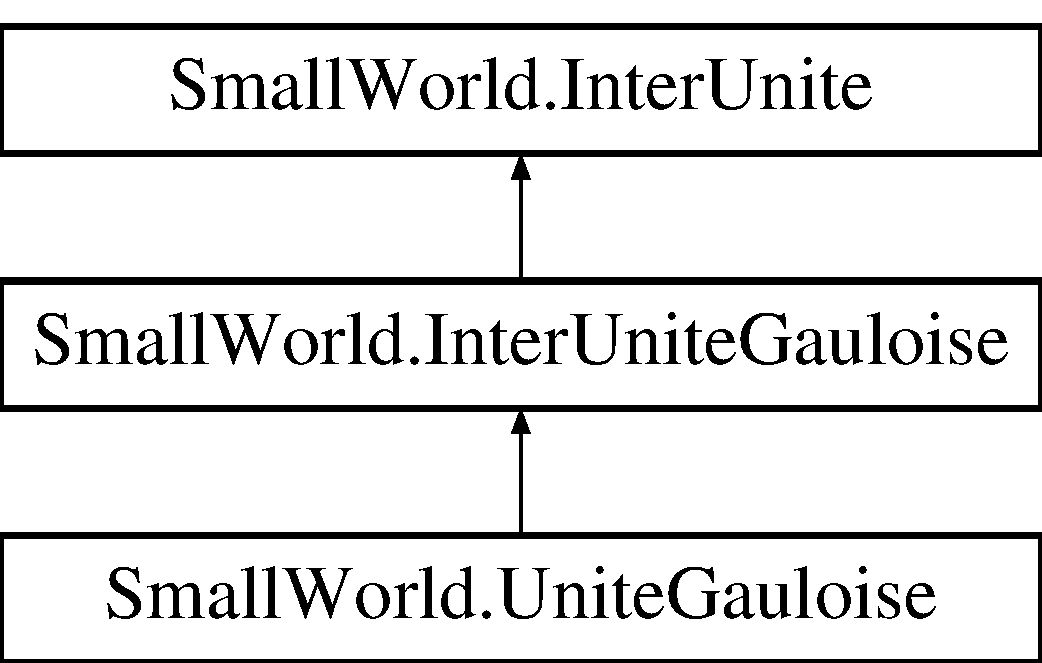
\includegraphics[height=3.000000cm]{interface_small_world_1_1_inter_unite_gauloise}
\end{center}
\end{figure}
\subsection*{Additional Inherited Members}


\subsection{Detailed Description}
Interface pour les unités gauloises. 

The documentation for this interface was generated from the following file\-:\begin{DoxyCompactItemize}
\item 
C\-:/\-Users/damienc/\-Documents/\-Git\-Hub/\-Small\-World/\-Visual\-Studio/\-Projet\-P\-O\-O/\hyperlink{_unite_8cs}{Unite.\-cs}\end{DoxyCompactItemize}

\hypertarget{interface_small_world_1_1_inter_unite_naine}{\section{Small\-World.\-Inter\-Unite\-Naine Interface Reference}
\label{interface_small_world_1_1_inter_unite_naine}\index{Small\-World.\-Inter\-Unite\-Naine@{Small\-World.\-Inter\-Unite\-Naine}}
}
Inheritance diagram for Small\-World.\-Inter\-Unite\-Naine\-:\begin{figure}[H]
\begin{center}
\leavevmode
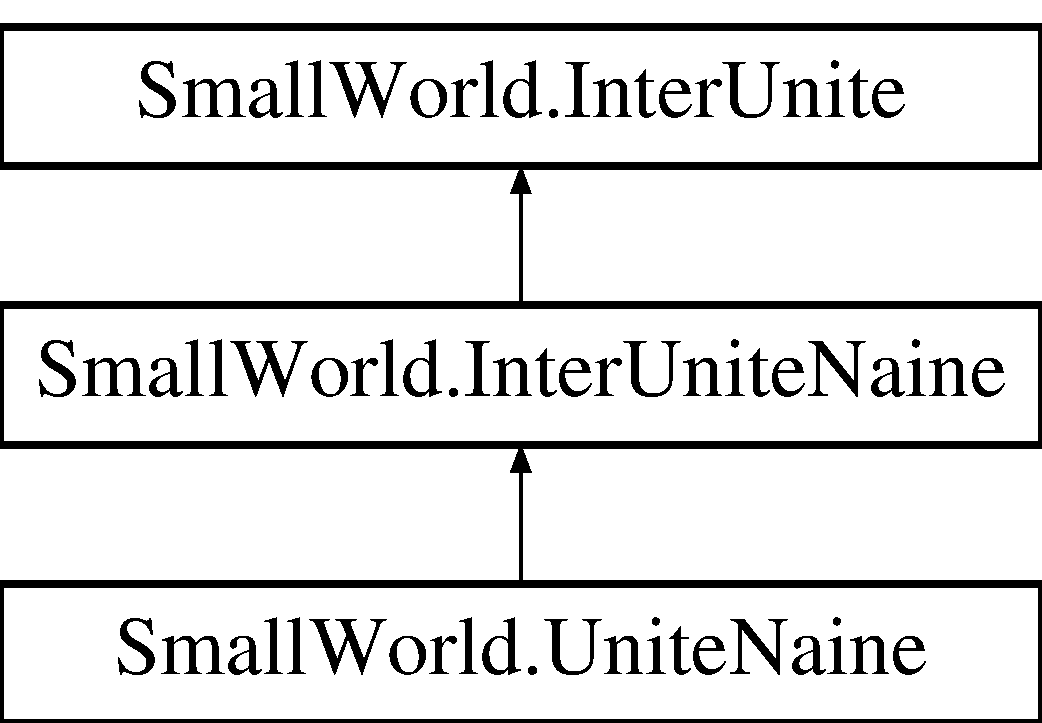
\includegraphics[height=3.000000cm]{interface_small_world_1_1_inter_unite_naine}
\end{center}
\end{figure}
\subsection*{Additional Inherited Members}


The documentation for this interface was generated from the following file\-:\begin{DoxyCompactItemize}
\item 
C\-:/\-Users/damienc/\-Documents/\-Git\-Hub/\-Small\-World/\-Visual\-Studio/\-Projet\-P\-O\-O/Unite\-Naine.\-cs\end{DoxyCompactItemize}

\hypertarget{interface_small_world_1_1_inter_unite_viking}{\section{Small\-World.\-Inter\-Unite\-Viking Interface Reference}
\label{interface_small_world_1_1_inter_unite_viking}\index{Small\-World.\-Inter\-Unite\-Viking@{Small\-World.\-Inter\-Unite\-Viking}}
}
Inheritance diagram for Small\-World.\-Inter\-Unite\-Viking\-:\begin{figure}[H]
\begin{center}
\leavevmode
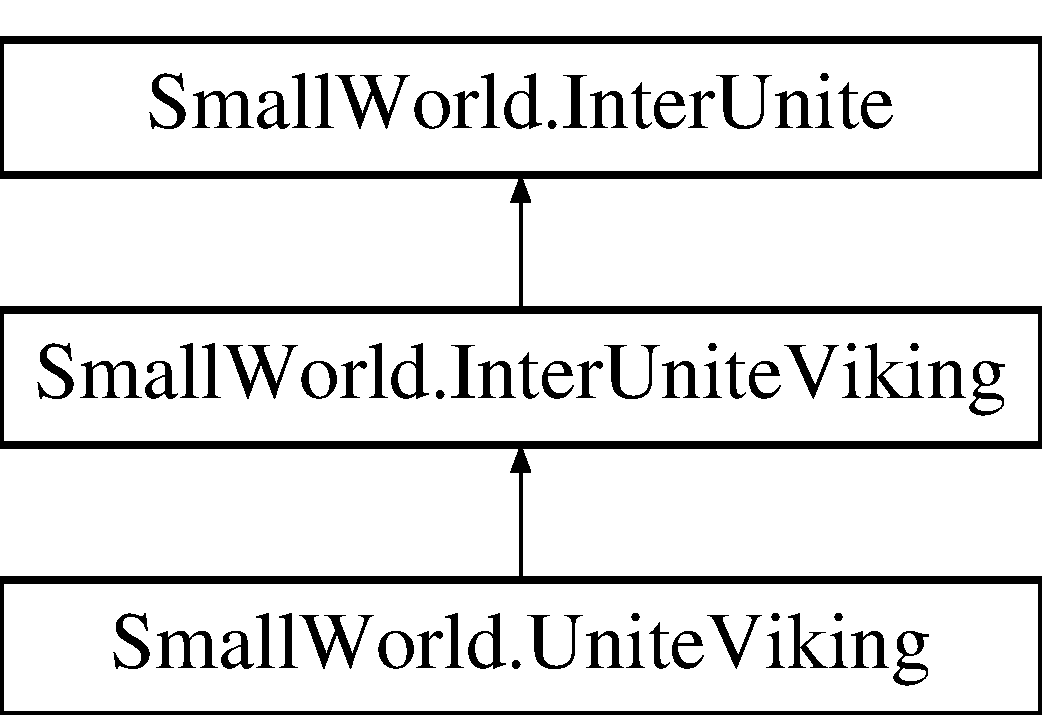
\includegraphics[height=3.000000cm]{interface_small_world_1_1_inter_unite_viking}
\end{center}
\end{figure}
\subsection*{Additional Inherited Members}


The documentation for this interface was generated from the following file\-:\begin{DoxyCompactItemize}
\item 
C\-:/\-Users/damienc/\-Documents/\-Git\-Hub/\-Small\-World/\-Visual\-Studio/\-Projet\-P\-O\-O/Unite\-Viking.\-cs\end{DoxyCompactItemize}

\hypertarget{class_small_world_1_1_joueur}{\section{Small\-World.\-Joueur Class Reference}
\label{class_small_world_1_1_joueur}\index{Small\-World.\-Joueur@{Small\-World.\-Joueur}}
}


classe pour un joueur  


Inheritance diagram for Small\-World.\-Joueur\-:\begin{figure}[H]
\begin{center}
\leavevmode
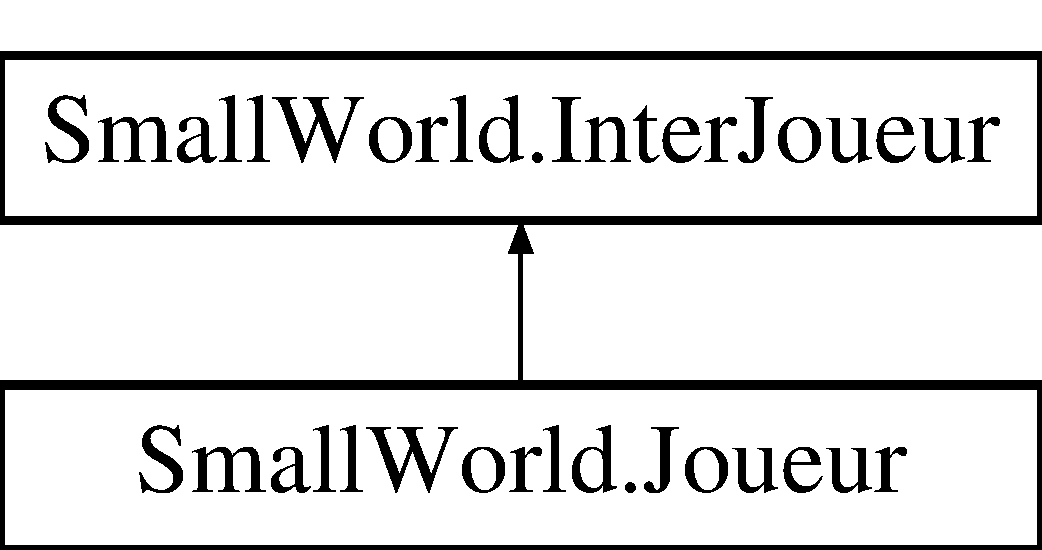
\includegraphics[height=2.000000cm]{class_small_world_1_1_joueur}
\end{center}
\end{figure}
\subsection*{Public Member Functions}
\begin{DoxyCompactItemize}
\item 
\hyperlink{class_small_world_1_1_joueur_ae9efc678037dc30e757898510cd4f9f2}{Joueur} (string nom, \hyperlink{class_small_world_1_1_peuple}{Peuple} nom\-Peuple)
\begin{DoxyCompactList}\small\item\em Constructeur d'un joueur. \end{DoxyCompactList}\item 
\hyperlink{class_small_world_1_1_joueur_a60844b7ba0c1294462c559644ed88bf1}{Joueur} ()
\begin{DoxyCompactList}\small\item\em Constructeur d'un joueur par défaut. \end{DoxyCompactList}\item 
void \hyperlink{class_small_world_1_1_joueur_aaa0f98cea097955f2c75e978433a7c68}{calculer\-Point\-Victoire} ()
\begin{DoxyCompactList}\small\item\em Met à jour les points de victoire du joueur. \end{DoxyCompactList}\end{DoxyCompactItemize}
\subsection*{Properties}
\begin{DoxyCompactItemize}
\item 
\hypertarget{class_small_world_1_1_joueur_ab6fe8c9fc5ad9925ec75b277e967c812}{\hyperlink{class_small_world_1_1_peuple}{Peuple} \hyperlink{class_small_world_1_1_joueur_ab6fe8c9fc5ad9925ec75b277e967c812}{Peuple\-J}\hspace{0.3cm}{\ttfamily  \mbox{[}get, set\mbox{]}}}\label{class_small_world_1_1_joueur_ab6fe8c9fc5ad9925ec75b277e967c812}

\begin{DoxyCompactList}\small\item\em \hyperlink{namespace_small_world_1_1_properties}{Properties} pour l'attribut peuple\-J. \end{DoxyCompactList}\item 
\hypertarget{class_small_world_1_1_joueur_a3d059cb06ae3403cd677ce2794635ae9}{int \hyperlink{class_small_world_1_1_joueur_a3d059cb06ae3403cd677ce2794635ae9}{Point\-Victoire}\hspace{0.3cm}{\ttfamily  \mbox{[}get, set\mbox{]}}}\label{class_small_world_1_1_joueur_a3d059cb06ae3403cd677ce2794635ae9}

\begin{DoxyCompactList}\small\item\em \hyperlink{namespace_small_world_1_1_properties}{Properties} pour l'attribut point\-Victoire. \end{DoxyCompactList}\item 
\hypertarget{class_small_world_1_1_joueur_aa5dd3c2c496b51bfd08470c1f24dabfa}{string \hyperlink{class_small_world_1_1_joueur_aa5dd3c2c496b51bfd08470c1f24dabfa}{Nom\-J}\hspace{0.3cm}{\ttfamily  \mbox{[}get, set\mbox{]}}}\label{class_small_world_1_1_joueur_aa5dd3c2c496b51bfd08470c1f24dabfa}

\begin{DoxyCompactList}\small\item\em \hyperlink{namespace_small_world_1_1_properties}{Properties} pour l'attribut nom\-J. \end{DoxyCompactList}\item 
\hypertarget{class_small_world_1_1_joueur_a0dd3a30f69558c1e72370445a94ce680}{List$<$ \hyperlink{class_small_world_1_1_unite}{Unite} $>$ {\bfseries Liste\-Unite}\hspace{0.3cm}{\ttfamily  \mbox{[}get, set\mbox{]}}}\label{class_small_world_1_1_joueur_a0dd3a30f69558c1e72370445a94ce680}

\end{DoxyCompactItemize}


\subsection{Detailed Description}
classe pour un joueur 

\subsection{Constructor \& Destructor Documentation}
\hypertarget{class_small_world_1_1_joueur_ae9efc678037dc30e757898510cd4f9f2}{\index{Small\-World\-::\-Joueur@{Small\-World\-::\-Joueur}!Joueur@{Joueur}}
\index{Joueur@{Joueur}!SmallWorld::Joueur@{Small\-World\-::\-Joueur}}
\subsubsection[{Joueur}]{\setlength{\rightskip}{0pt plus 5cm}Small\-World.\-Joueur.\-Joueur (
\begin{DoxyParamCaption}
\item[{string}]{nom, }
\item[{{\bf Peuple}}]{nom\-Peuple}
\end{DoxyParamCaption}
)}}\label{class_small_world_1_1_joueur_ae9efc678037dc30e757898510cd4f9f2}


Constructeur d'un joueur. 

Crée le joueur à partir de son nom et de son peuple


\begin{DoxyParams}{Parameters}
{\em string} & {\bfseries nom} le nom du joueur \\
\hline
{\em \hyperlink{class_small_world_1_1_peuple}{Peuple}} & {\bfseries nom\-Peuple} le peuple sélectionné par le joueur \\
\hline
\end{DoxyParams}
\hypertarget{class_small_world_1_1_joueur_a60844b7ba0c1294462c559644ed88bf1}{\index{Small\-World\-::\-Joueur@{Small\-World\-::\-Joueur}!Joueur@{Joueur}}
\index{Joueur@{Joueur}!SmallWorld::Joueur@{Small\-World\-::\-Joueur}}
\subsubsection[{Joueur}]{\setlength{\rightskip}{0pt plus 5cm}Small\-World.\-Joueur.\-Joueur (
\begin{DoxyParamCaption}
{}
\end{DoxyParamCaption}
)}}\label{class_small_world_1_1_joueur_a60844b7ba0c1294462c559644ed88bf1}


Constructeur d'un joueur par défaut. 

\begin{DoxyReturn}{Returns}
\hyperlink{class_small_world_1_1_joueur}{Joueur} un nouveau joueur 
\end{DoxyReturn}


\subsection{Member Function Documentation}
\hypertarget{class_small_world_1_1_joueur_aaa0f98cea097955f2c75e978433a7c68}{\index{Small\-World\-::\-Joueur@{Small\-World\-::\-Joueur}!calculer\-Point\-Victoire@{calculer\-Point\-Victoire}}
\index{calculer\-Point\-Victoire@{calculer\-Point\-Victoire}!SmallWorld::Joueur@{Small\-World\-::\-Joueur}}
\subsubsection[{calculer\-Point\-Victoire}]{\setlength{\rightskip}{0pt plus 5cm}Small\-World.\-Joueur.\-calculer\-Point\-Victoire (
\begin{DoxyParamCaption}
{}
\end{DoxyParamCaption}
)}}\label{class_small_world_1_1_joueur_aaa0f98cea097955f2c75e978433a7c68}


Met à jour les points de victoire du joueur. 

\begin{DoxyReturn}{Returns}
void 
\end{DoxyReturn}


Implements \hyperlink{interface_small_world_1_1_inter_joueur_affcd2a1f3208993fd9fd5f78b4873b70}{Small\-World.\-Inter\-Joueur}.



The documentation for this class was generated from the following file\-:\begin{DoxyCompactItemize}
\item 
C\-:/\-Users/damienc/\-Documents/\-Git\-Hub/\-Small\-World/\-Visual\-Studio/\-Projet\-P\-O\-O/\hyperlink{_joueur_8cs}{Joueur.\-cs}\end{DoxyCompactItemize}

\hypertarget{class_small_world_1_1_montagne}{\section{Small\-World.\-Montagne Class Reference}
\label{class_small_world_1_1_montagne}\index{Small\-World.\-Montagne@{Small\-World.\-Montagne}}
}
Inheritance diagram for Small\-World.\-Montagne\-:\begin{figure}[H]
\begin{center}
\leavevmode
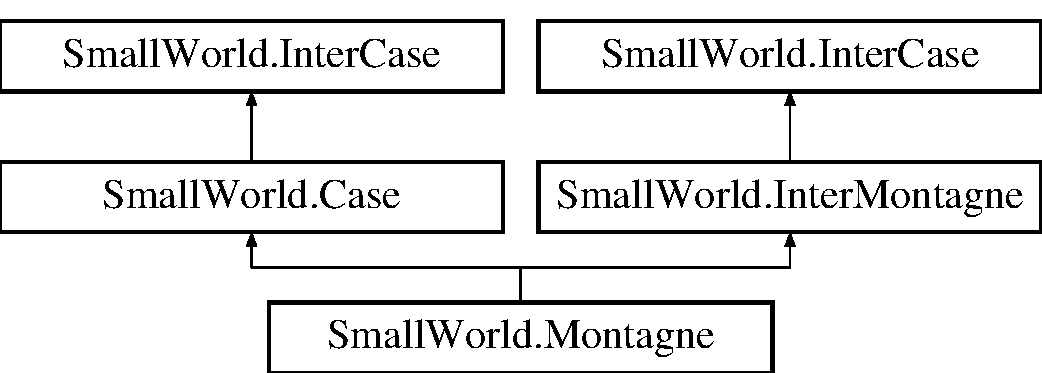
\includegraphics[height=3.000000cm]{class_small_world_1_1_montagne}
\end{center}
\end{figure}
\subsection*{Additional Inherited Members}


The documentation for this class was generated from the following file\-:\begin{DoxyCompactItemize}
\item 
C\-:/\-Users/damienc/\-Documents/\-Git\-Hub/\-Small\-World/\-Visual\-Studio/\-Projet\-P\-O\-O/Case.\-cs\end{DoxyCompactItemize}

\hypertarget{class_small_world_1_1_monteur_partie}{\section{Small\-World.\-Monteur\-Partie Class Reference}
\label{class_small_world_1_1_monteur_partie}\index{Small\-World.\-Monteur\-Partie@{Small\-World.\-Monteur\-Partie}}
}
Inheritance diagram for Small\-World.\-Monteur\-Partie\-:\begin{figure}[H]
\begin{center}
\leavevmode
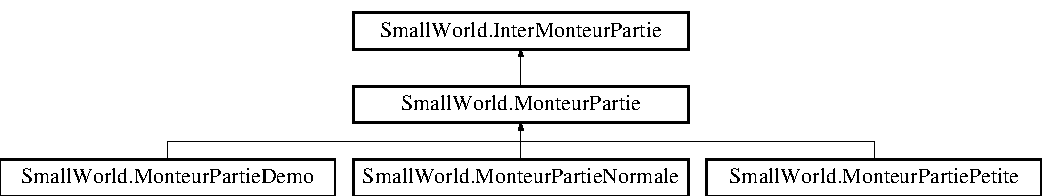
\includegraphics[height=2.616822cm]{class_small_world_1_1_monteur_partie}
\end{center}
\end{figure}
\subsection*{Public Member Functions}
\begin{DoxyCompactItemize}
\item 
\hypertarget{class_small_world_1_1_monteur_partie_ad64e720f9f051d0f17eb134d0c112e73}{void {\bfseries ajouter\-Carte} ()}\label{class_small_world_1_1_monteur_partie_ad64e720f9f051d0f17eb134d0c112e73}

\item 
\hypertarget{class_small_world_1_1_monteur_partie_a7e2370c4e2de6e0885a18bdcece42e0f}{void {\bfseries ajouter\-Joueur} ()}\label{class_small_world_1_1_monteur_partie_a7e2370c4e2de6e0885a18bdcece42e0f}

\item 
\hypertarget{class_small_world_1_1_monteur_partie_ab77c0f384bbc52765d1462173e03b9b5}{\hyperlink{interface_small_world_1_1_partie}{Small\-World.\-Partie} \hyperlink{class_small_world_1_1_monteur_partie_ab77c0f384bbc52765d1462173e03b9b5}{creer\-Partie} ()}\label{class_small_world_1_1_monteur_partie_ab77c0f384bbc52765d1462173e03b9b5}

\begin{DoxyCompactList}\small\item\em Création la partie. \end{DoxyCompactList}\item 
\hypertarget{class_small_world_1_1_monteur_partie_a0f15d1583b4289efb1ed7e9bba11d897}{void \hyperlink{class_small_world_1_1_monteur_partie_a0f15d1583b4289efb1ed7e9bba11d897}{placer\-Unites} ()}\label{class_small_world_1_1_monteur_partie_a0f15d1583b4289efb1ed7e9bba11d897}

\begin{DoxyCompactList}\small\item\em Placement des unités avant le début de la partie. \end{DoxyCompactList}\end{DoxyCompactItemize}


The documentation for this class was generated from the following file\-:\begin{DoxyCompactItemize}
\item 
C\-:/\-Users/damienc/\-Documents/\-Git\-Hub/\-Small\-World/\-Visual\-Studio/\-Projet\-P\-O\-O/\hyperlink{_monteur_partie_8cs}{Monteur\-Partie.\-cs}\end{DoxyCompactItemize}

\hypertarget{class_small_world_1_1_monteur_partie_demo}{\section{Small\-World.\-Monteur\-Partie\-Demo Class Reference}
\label{class_small_world_1_1_monteur_partie_demo}\index{Small\-World.\-Monteur\-Partie\-Demo@{Small\-World.\-Monteur\-Partie\-Demo}}
}
Inheritance diagram for Small\-World.\-Monteur\-Partie\-Demo\-:\begin{figure}[H]
\begin{center}
\leavevmode
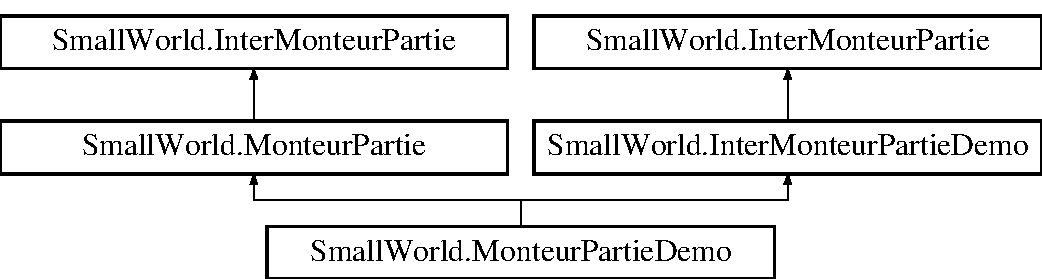
\includegraphics[height=3.000000cm]{class_small_world_1_1_monteur_partie_demo}
\end{center}
\end{figure}
\subsection*{Public Member Functions}
\begin{DoxyCompactItemize}
\item 
\hypertarget{class_small_world_1_1_monteur_partie_demo_a46b397bf827fae4e88d4b7d8e05e6a12}{void {\bfseries ajouter\-Peuple} ()}\label{class_small_world_1_1_monteur_partie_demo_a46b397bf827fae4e88d4b7d8e05e6a12}

\item 
\hypertarget{class_small_world_1_1_monteur_partie_demo_a5efd564916b7517ef2466d7d978258ad}{\hyperlink{interface_small_world_1_1_partie}{Small\-World.\-Partie} \hyperlink{class_small_world_1_1_monteur_partie_demo_a5efd564916b7517ef2466d7d978258ad}{creer\-Partie} ()}\label{class_small_world_1_1_monteur_partie_demo_a5efd564916b7517ef2466d7d978258ad}

\begin{DoxyCompactList}\small\item\em Création la partie. \end{DoxyCompactList}\item 
\hypertarget{class_small_world_1_1_monteur_partie_demo_ac94cddf22f61463798b47d7ff609ba06}{void {\bfseries ajouter\-Carte} ()}\label{class_small_world_1_1_monteur_partie_demo_ac94cddf22f61463798b47d7ff609ba06}

\item 
\hypertarget{class_small_world_1_1_monteur_partie_demo_a13aea66c36b2d14f7103e227a8cabdd1}{void {\bfseries ajouter\-Joueur} ()}\label{class_small_world_1_1_monteur_partie_demo_a13aea66c36b2d14f7103e227a8cabdd1}

\item 
\hypertarget{class_small_world_1_1_monteur_partie_demo_a24388e70f314a661cbcaeffbc4535c83}{void \hyperlink{class_small_world_1_1_monteur_partie_demo_a24388e70f314a661cbcaeffbc4535c83}{placer\-Unites} ()}\label{class_small_world_1_1_monteur_partie_demo_a24388e70f314a661cbcaeffbc4535c83}

\begin{DoxyCompactList}\small\item\em Placement des unités avant le début de la partie. \end{DoxyCompactList}\end{DoxyCompactItemize}


The documentation for this class was generated from the following file\-:\begin{DoxyCompactItemize}
\item 
C\-:/\-Users/damienc/\-Documents/\-Git\-Hub/\-Small\-World/\-Visual\-Studio/\-Projet\-P\-O\-O/\hyperlink{_monteur_partie_8cs}{Monteur\-Partie.\-cs}\end{DoxyCompactItemize}

\hypertarget{class_small_world_1_1_monteur_partie_normale}{\section{Small\-World.\-Monteur\-Partie\-Normale Class Reference}
\label{class_small_world_1_1_monteur_partie_normale}\index{Small\-World.\-Monteur\-Partie\-Normale@{Small\-World.\-Monteur\-Partie\-Normale}}
}
Inheritance diagram for Small\-World.\-Monteur\-Partie\-Normale\-:\begin{figure}[H]
\begin{center}
\leavevmode
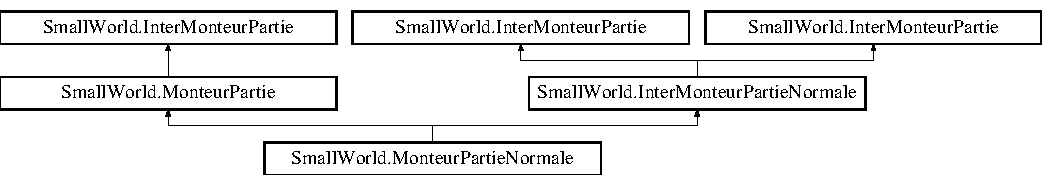
\includegraphics[height=2.343096cm]{class_small_world_1_1_monteur_partie_normale}
\end{center}
\end{figure}
\subsection*{Public Member Functions}
\begin{DoxyCompactItemize}
\item 
\hypertarget{class_small_world_1_1_monteur_partie_normale_a095529a4b08f7227415e960e7edf4be4}{void {\bfseries ajouter\-Peuple} ()}\label{class_small_world_1_1_monteur_partie_normale_a095529a4b08f7227415e960e7edf4be4}

\item 
\hypertarget{class_small_world_1_1_monteur_partie_normale_a27f7e7f429852ea6f543593d09b31f93}{\hyperlink{interface_small_world_1_1_partie}{Small\-World.\-Partie} \hyperlink{class_small_world_1_1_monteur_partie_normale_a27f7e7f429852ea6f543593d09b31f93}{creer\-Partie} ()}\label{class_small_world_1_1_monteur_partie_normale_a27f7e7f429852ea6f543593d09b31f93}

\begin{DoxyCompactList}\small\item\em Création la partie. \end{DoxyCompactList}\item 
\hypertarget{class_small_world_1_1_monteur_partie_normale_a9f6a6e1e348fa3d971ee8a409e986c55}{void {\bfseries ajouter\-Carte} ()}\label{class_small_world_1_1_monteur_partie_normale_a9f6a6e1e348fa3d971ee8a409e986c55}

\item 
\hypertarget{class_small_world_1_1_monteur_partie_normale_a6ba30a3502a862c7943ba991eacc2fb0}{void {\bfseries ajouter\-Joueur} ()}\label{class_small_world_1_1_monteur_partie_normale_a6ba30a3502a862c7943ba991eacc2fb0}

\item 
\hypertarget{class_small_world_1_1_monteur_partie_normale_a79b156ac66696c5bce20cb025a39f1ce}{void \hyperlink{class_small_world_1_1_monteur_partie_normale_a79b156ac66696c5bce20cb025a39f1ce}{placer\-Unites} ()}\label{class_small_world_1_1_monteur_partie_normale_a79b156ac66696c5bce20cb025a39f1ce}

\begin{DoxyCompactList}\small\item\em Placement des unités avant le début de la partie. \end{DoxyCompactList}\end{DoxyCompactItemize}


The documentation for this class was generated from the following file\-:\begin{DoxyCompactItemize}
\item 
C\-:/\-Users/damienc/\-Documents/\-Git\-Hub/\-Small\-World/\-Visual\-Studio/\-Projet\-P\-O\-O/\hyperlink{_monteur_partie_8cs}{Monteur\-Partie.\-cs}\end{DoxyCompactItemize}

\hypertarget{class_small_world_1_1_monteur_partie_petite}{\section{Small\-World.\-Monteur\-Partie\-Petite Class Reference}
\label{class_small_world_1_1_monteur_partie_petite}\index{Small\-World.\-Monteur\-Partie\-Petite@{Small\-World.\-Monteur\-Partie\-Petite}}
}
Inheritance diagram for Small\-World.\-Monteur\-Partie\-Petite\-:\begin{figure}[H]
\begin{center}
\leavevmode
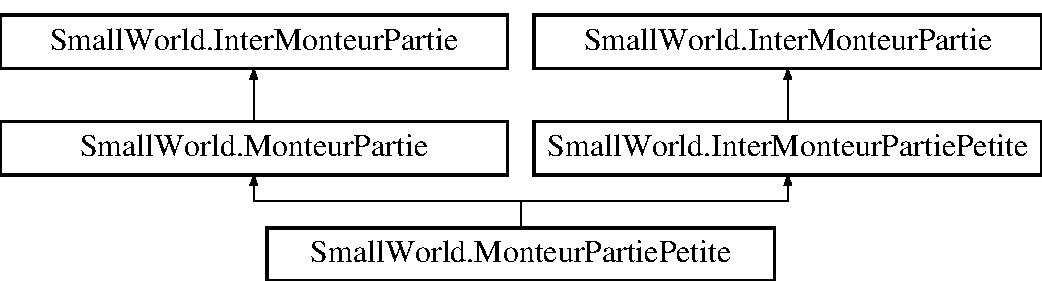
\includegraphics[height=3.000000cm]{class_small_world_1_1_monteur_partie_petite}
\end{center}
\end{figure}
\subsection*{Public Member Functions}
\begin{DoxyCompactItemize}
\item 
\hypertarget{class_small_world_1_1_monteur_partie_petite_aa2a1e673524ca4bc7c3a4fece40e5897}{void {\bfseries ajouter\-Peuple} ()}\label{class_small_world_1_1_monteur_partie_petite_aa2a1e673524ca4bc7c3a4fece40e5897}

\item 
\hypertarget{class_small_world_1_1_monteur_partie_petite_a4ed51a6a8910b8bf477dba7dd2632435}{\hyperlink{interface_small_world_1_1_partie}{Small\-World.\-Partie} \hyperlink{class_small_world_1_1_monteur_partie_petite_a4ed51a6a8910b8bf477dba7dd2632435}{creer\-Partie} ()}\label{class_small_world_1_1_monteur_partie_petite_a4ed51a6a8910b8bf477dba7dd2632435}

\begin{DoxyCompactList}\small\item\em Création la partie. \end{DoxyCompactList}\item 
\hypertarget{class_small_world_1_1_monteur_partie_petite_a0d2cb43e852d988eb059d9e2c7189daa}{void {\bfseries ajouter\-Carte} ()}\label{class_small_world_1_1_monteur_partie_petite_a0d2cb43e852d988eb059d9e2c7189daa}

\item 
\hypertarget{class_small_world_1_1_monteur_partie_petite_ad09f7febe49248965e49a20aa59a77d4}{void {\bfseries ajouter\-Joueur} ()}\label{class_small_world_1_1_monteur_partie_petite_ad09f7febe49248965e49a20aa59a77d4}

\item 
\hypertarget{class_small_world_1_1_monteur_partie_petite_aff25e14f2ebe9bbb915c211dc759bf1e}{void \hyperlink{class_small_world_1_1_monteur_partie_petite_aff25e14f2ebe9bbb915c211dc759bf1e}{placer\-Unites} ()}\label{class_small_world_1_1_monteur_partie_petite_aff25e14f2ebe9bbb915c211dc759bf1e}

\begin{DoxyCompactList}\small\item\em Placement des unités avant le début de la partie. \end{DoxyCompactList}\end{DoxyCompactItemize}


The documentation for this class was generated from the following file\-:\begin{DoxyCompactItemize}
\item 
C\-:/\-Users/damienc/\-Documents/\-Git\-Hub/\-Small\-World/\-Visual\-Studio/\-Projet\-P\-O\-O/\hyperlink{_monteur_partie_8cs}{Monteur\-Partie.\-cs}\end{DoxyCompactItemize}

\hypertarget{class_small_world_1_1_partie}{\section{Small\-World.\-Partie Class Reference}
\label{class_small_world_1_1_partie}\index{Small\-World.\-Partie@{Small\-World.\-Partie}}
}
Inheritance diagram for Small\-World.\-Partie\-:\begin{figure}[H]
\begin{center}
\leavevmode
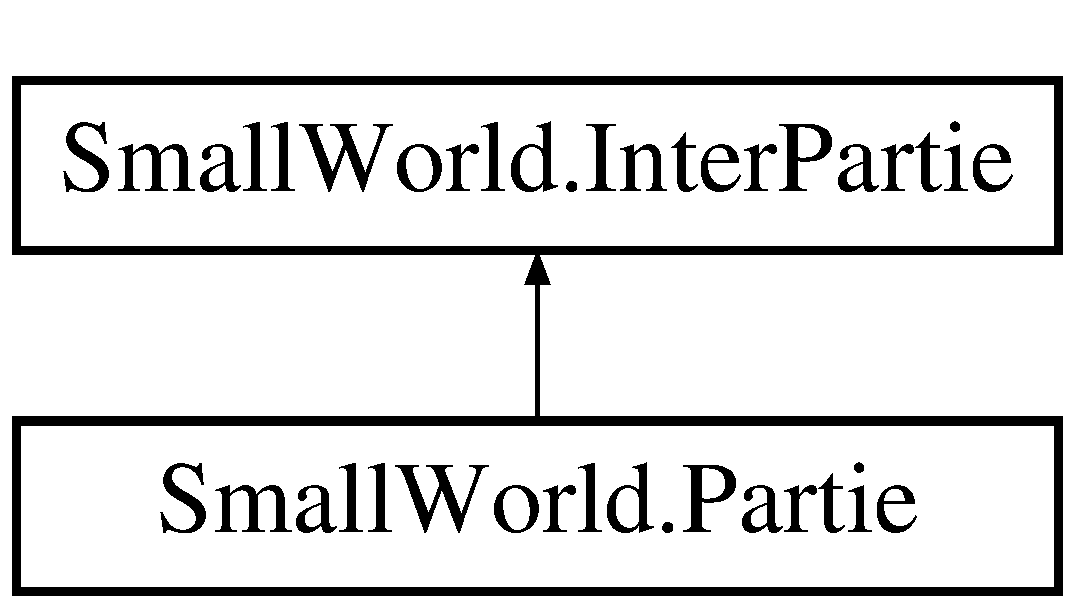
\includegraphics[height=2.000000cm]{class_small_world_1_1_partie}
\end{center}
\end{figure}
\subsection*{Public Member Functions}
\begin{DoxyCompactItemize}
\item 
\hypertarget{class_small_world_1_1_partie_a6123fa8d79551c91a92c7832649225b9}{void {\bfseries nouveau\-Tour} ()}\label{class_small_world_1_1_partie_a6123fa8d79551c91a92c7832649225b9}

\item 
\hypertarget{class_small_world_1_1_partie_aa76d3d1509ecdcb35fed3621455bab9f}{void {\bfseries selectionner\-Unite} ()}\label{class_small_world_1_1_partie_aa76d3d1509ecdcb35fed3621455bab9f}

\item 
\hypertarget{class_small_world_1_1_partie_abc458c09d880b2b16502bfe695439195}{void {\bfseries demander\-Deplacement} ()}\label{class_small_world_1_1_partie_abc458c09d880b2b16502bfe695439195}

\item 
\hypertarget{class_small_world_1_1_partie_a7ddc97d7833d234e06f18f0a97c6c15e}{void {\bfseries valider\-Tour} ()}\label{class_small_world_1_1_partie_a7ddc97d7833d234e06f18f0a97c6c15e}

\end{DoxyCompactItemize}
\subsection*{Properties}
\begin{DoxyCompactItemize}
\item 
\hypertarget{class_small_world_1_1_partie_a204fb33757e7ab7d0427a3c37f938062}{\hyperlink{class_small_world_1_1_joueur}{Joueur} {\bfseries Joueur}\hspace{0.3cm}{\ttfamily  \mbox{[}get, set\mbox{]}}}\label{class_small_world_1_1_partie_a204fb33757e7ab7d0427a3c37f938062}

\item 
\hypertarget{class_small_world_1_1_partie_a62ae701f7e4fa523001a6326c0033e6b}{\hyperlink{class_small_world_1_1_carte}{Carte} {\bfseries Carte}\hspace{0.3cm}{\ttfamily  \mbox{[}get, set\mbox{]}}}\label{class_small_world_1_1_partie_a62ae701f7e4fa523001a6326c0033e6b}

\item 
\hypertarget{class_small_world_1_1_partie_a76f9f56c84f30004462e65de85cbd1e3}{int {\bfseries nb\-Tour\-Restant}\hspace{0.3cm}{\ttfamily  \mbox{[}get, set\mbox{]}}}\label{class_small_world_1_1_partie_a76f9f56c84f30004462e65de85cbd1e3}

\end{DoxyCompactItemize}


The documentation for this class was generated from the following file\-:\begin{DoxyCompactItemize}
\item 
C\-:/\-Users/damienc/\-Documents/\-Git\-Hub/\-Small\-World/\-Visual\-Studio/\-Projet\-P\-O\-O/Partie.\-cs\end{DoxyCompactItemize}

\hypertarget{class_small_world_1_1_peuple}{\section{Small\-World.\-Peuple Class Reference}
\label{class_small_world_1_1_peuple}\index{Small\-World.\-Peuple@{Small\-World.\-Peuple}}
}
Inheritance diagram for Small\-World.\-Peuple\-:\begin{figure}[H]
\begin{center}
\leavevmode
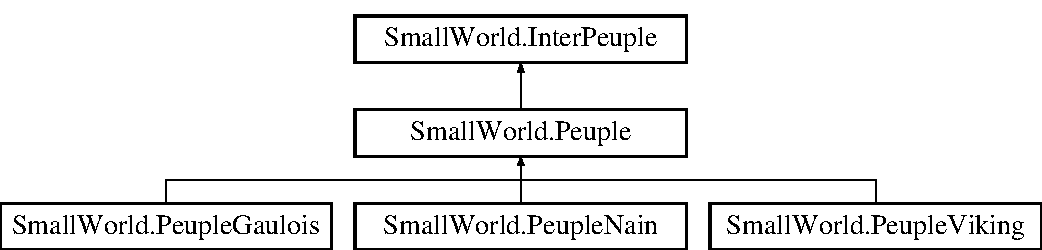
\includegraphics[height=3.000000cm]{class_small_world_1_1_peuple}
\end{center}
\end{figure}
\subsection*{Public Member Functions}
\begin{DoxyCompactItemize}
\item 
\hypertarget{class_small_world_1_1_peuple_ae780348f6362ec2b371f58f0a2f696a1}{\hyperlink{interface_small_world_1_1_inter_unite}{Inter\-Unite} {\bfseries creer\-Unite} ()}\label{class_small_world_1_1_peuple_ae780348f6362ec2b371f58f0a2f696a1}

\end{DoxyCompactItemize}


The documentation for this class was generated from the following file\-:\begin{DoxyCompactItemize}
\item 
C\-:/\-Users/damienc/\-Documents/\-Git\-Hub/\-Small\-World/\-Visual\-Studio/\-Projet\-P\-O\-O/Peuple.\-cs\end{DoxyCompactItemize}

\hypertarget{class_small_world_1_1_peuple_gaulois}{\section{Small\-World.\-Peuple\-Gaulois Class Reference}
\label{class_small_world_1_1_peuple_gaulois}\index{Small\-World.\-Peuple\-Gaulois@{Small\-World.\-Peuple\-Gaulois}}
}


classe pour le peuple Gaulois  


Inheritance diagram for Small\-World.\-Peuple\-Gaulois\-:\begin{figure}[H]
\begin{center}
\leavevmode
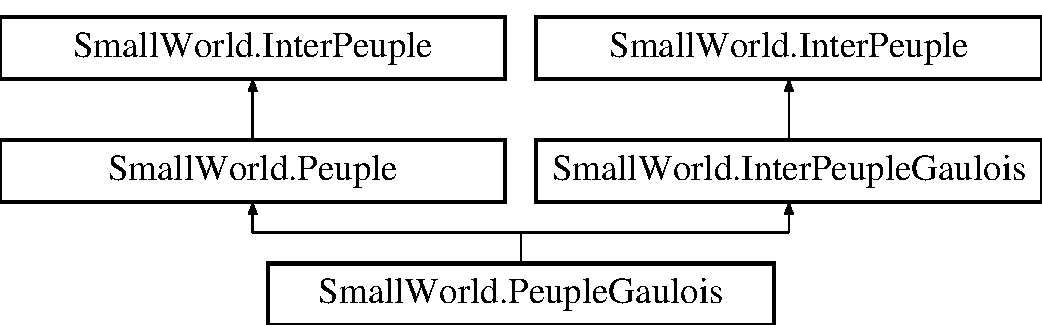
\includegraphics[height=3.000000cm]{class_small_world_1_1_peuple_gaulois}
\end{center}
\end{figure}
\subsection*{Public Member Functions}
\begin{DoxyCompactItemize}
\item 
\hyperlink{class_small_world_1_1_peuple_gaulois_a3d978359df0903934b95a0507ca409e2}{Peuple\-Gaulois} ()
\begin{DoxyCompactList}\small\item\em Constructeur d'un peuple gaulois. \end{DoxyCompactList}\item 
override \hyperlink{class_small_world_1_1_unite}{Unite} \hyperlink{class_small_world_1_1_peuple_gaulois_aac9e86d3354a8c4e588a942c705539ee}{creer\-Unite} ()
\begin{DoxyCompactList}\small\item\em création d'une unité gauloise \end{DoxyCompactList}\end{DoxyCompactItemize}


\subsection{Detailed Description}
classe pour le peuple Gaulois 

\subsection{Constructor \& Destructor Documentation}
\hypertarget{class_small_world_1_1_peuple_gaulois_a3d978359df0903934b95a0507ca409e2}{\index{Small\-World\-::\-Peuple\-Gaulois@{Small\-World\-::\-Peuple\-Gaulois}!Peuple\-Gaulois@{Peuple\-Gaulois}}
\index{Peuple\-Gaulois@{Peuple\-Gaulois}!SmallWorld::PeupleGaulois@{Small\-World\-::\-Peuple\-Gaulois}}
\subsubsection[{Peuple\-Gaulois}]{\setlength{\rightskip}{0pt plus 5cm}Small\-World.\-Peuple\-Gaulois.\-Peuple\-Gaulois (
\begin{DoxyParamCaption}
{}
\end{DoxyParamCaption}
)}}\label{class_small_world_1_1_peuple_gaulois_a3d978359df0903934b95a0507ca409e2}


Constructeur d'un peuple gaulois. 

\begin{DoxyReturn}{Returns}
\hyperlink{class_small_world_1_1_peuple_gaulois}{Peuple\-Gaulois} un peuple gaulois 
\end{DoxyReturn}


\subsection{Member Function Documentation}
\hypertarget{class_small_world_1_1_peuple_gaulois_aac9e86d3354a8c4e588a942c705539ee}{\index{Small\-World\-::\-Peuple\-Gaulois@{Small\-World\-::\-Peuple\-Gaulois}!creer\-Unite@{creer\-Unite}}
\index{creer\-Unite@{creer\-Unite}!SmallWorld::PeupleGaulois@{Small\-World\-::\-Peuple\-Gaulois}}
\subsubsection[{creer\-Unite}]{\setlength{\rightskip}{0pt plus 5cm}Small\-World.\-Peuple\-Gaulois.\-creer\-Unite (
\begin{DoxyParamCaption}
{}
\end{DoxyParamCaption}
)\hspace{0.3cm}{\ttfamily [virtual]}}}\label{class_small_world_1_1_peuple_gaulois_aac9e86d3354a8c4e588a942c705539ee}


création d'une unité gauloise 

\begin{DoxyReturn}{Returns}
\hyperlink{class_small_world_1_1_unite}{Unite} une nouvelle unité 
\end{DoxyReturn}


Implements \hyperlink{class_small_world_1_1_peuple_a9d7edd46744bf12c7592b93342835a9b}{Small\-World.\-Peuple}.



The documentation for this class was generated from the following file\-:\begin{DoxyCompactItemize}
\item 
C\-:/\-Users/damienc/\-Documents/\-Git\-Hub/\-Small\-World/\-Visual\-Studio/\-Projet\-P\-O\-O/\hyperlink{_peuple_8cs}{Peuple.\-cs}\end{DoxyCompactItemize}

\hypertarget{class_small_world_1_1_peuple_nain}{\section{Small\-World.\-Peuple\-Nain Class Reference}
\label{class_small_world_1_1_peuple_nain}\index{Small\-World.\-Peuple\-Nain@{Small\-World.\-Peuple\-Nain}}
}


classe pour le peuple nain  


Inheritance diagram for Small\-World.\-Peuple\-Nain\-:\begin{figure}[H]
\begin{center}
\leavevmode
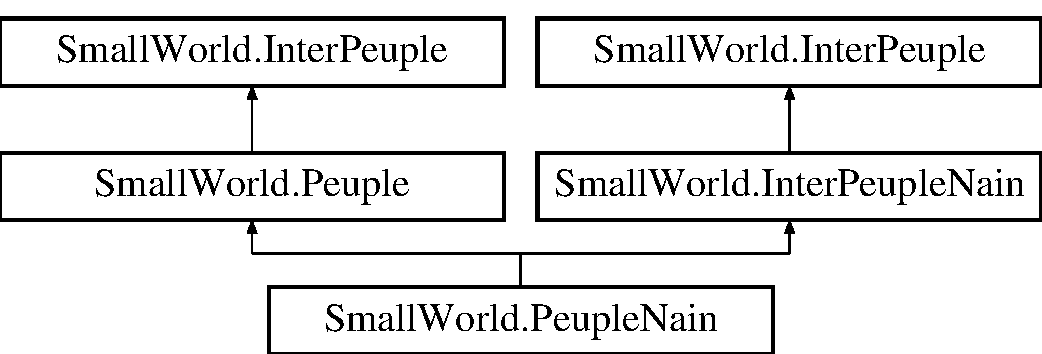
\includegraphics[height=3.000000cm]{class_small_world_1_1_peuple_nain}
\end{center}
\end{figure}
\subsection*{Public Member Functions}
\begin{DoxyCompactItemize}
\item 
\hyperlink{class_small_world_1_1_peuple_nain_a8d095e5799eec199c584195df7a4d237}{Peuple\-Nain} ()
\begin{DoxyCompactList}\small\item\em Constructeur d'un peuple nain. \end{DoxyCompactList}\item 
override \hyperlink{class_small_world_1_1_unite}{Unite} \hyperlink{class_small_world_1_1_peuple_nain_a31cf5c32229c6f88acf69de84a8c6ebf}{creer\-Unite} ()
\begin{DoxyCompactList}\small\item\em création d'une unité naine \end{DoxyCompactList}\end{DoxyCompactItemize}


\subsection{Detailed Description}
classe pour le peuple nain 

\subsection{Constructor \& Destructor Documentation}
\hypertarget{class_small_world_1_1_peuple_nain_a8d095e5799eec199c584195df7a4d237}{\index{Small\-World\-::\-Peuple\-Nain@{Small\-World\-::\-Peuple\-Nain}!Peuple\-Nain@{Peuple\-Nain}}
\index{Peuple\-Nain@{Peuple\-Nain}!SmallWorld::PeupleNain@{Small\-World\-::\-Peuple\-Nain}}
\subsubsection[{Peuple\-Nain}]{\setlength{\rightskip}{0pt plus 5cm}Small\-World.\-Peuple\-Nain.\-Peuple\-Nain (
\begin{DoxyParamCaption}
{}
\end{DoxyParamCaption}
)}}\label{class_small_world_1_1_peuple_nain_a8d095e5799eec199c584195df7a4d237}


Constructeur d'un peuple nain. 

\begin{DoxyReturn}{Returns}
\hyperlink{class_small_world_1_1_peuple_nain}{Peuple\-Nain} un peuple nain 
\end{DoxyReturn}


\subsection{Member Function Documentation}
\hypertarget{class_small_world_1_1_peuple_nain_a31cf5c32229c6f88acf69de84a8c6ebf}{\index{Small\-World\-::\-Peuple\-Nain@{Small\-World\-::\-Peuple\-Nain}!creer\-Unite@{creer\-Unite}}
\index{creer\-Unite@{creer\-Unite}!SmallWorld::PeupleNain@{Small\-World\-::\-Peuple\-Nain}}
\subsubsection[{creer\-Unite}]{\setlength{\rightskip}{0pt plus 5cm}Small\-World.\-Peuple\-Nain.\-creer\-Unite (
\begin{DoxyParamCaption}
{}
\end{DoxyParamCaption}
)\hspace{0.3cm}{\ttfamily [virtual]}}}\label{class_small_world_1_1_peuple_nain_a31cf5c32229c6f88acf69de84a8c6ebf}


création d'une unité naine 

\begin{DoxyReturn}{Returns}
\hyperlink{class_small_world_1_1_unite}{Unite} une nouvelle unité 
\end{DoxyReturn}


Implements \hyperlink{class_small_world_1_1_peuple_a9d7edd46744bf12c7592b93342835a9b}{Small\-World.\-Peuple}.



The documentation for this class was generated from the following file\-:\begin{DoxyCompactItemize}
\item 
C\-:/\-Users/damienc/\-Documents/\-Git\-Hub/\-Small\-World/\-Visual\-Studio/\-Projet\-P\-O\-O/\hyperlink{_peuple_8cs}{Peuple.\-cs}\end{DoxyCompactItemize}

\hypertarget{class_small_world_1_1_peuple_viking}{\section{Small\-World.\-Peuple\-Viking Class Reference}
\label{class_small_world_1_1_peuple_viking}\index{Small\-World.\-Peuple\-Viking@{Small\-World.\-Peuple\-Viking}}
}


classe pour le peuple viking  


Inheritance diagram for Small\-World.\-Peuple\-Viking\-:\begin{figure}[H]
\begin{center}
\leavevmode
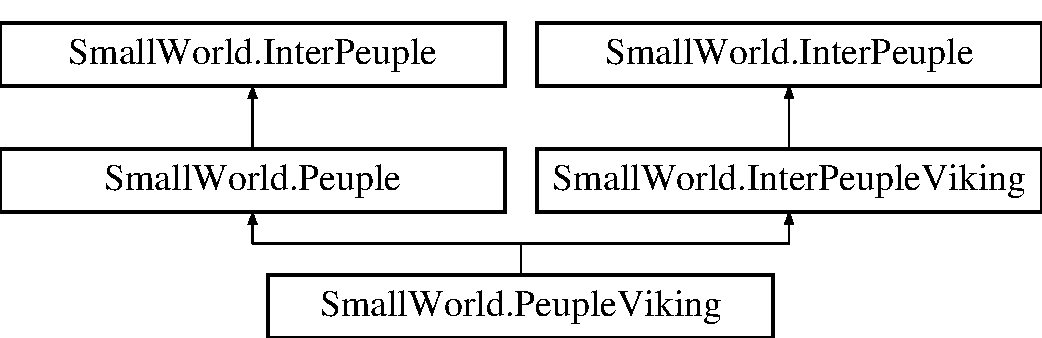
\includegraphics[height=3.000000cm]{class_small_world_1_1_peuple_viking}
\end{center}
\end{figure}
\subsection*{Public Member Functions}
\begin{DoxyCompactItemize}
\item 
\hyperlink{class_small_world_1_1_peuple_viking_aed3d04f06df7dadd594ede3f986d9ab1}{Peuple\-Viking} ()
\begin{DoxyCompactList}\small\item\em Constructeur d'un peuple viking. \end{DoxyCompactList}\item 
override \hyperlink{class_small_world_1_1_unite}{Unite} \hyperlink{class_small_world_1_1_peuple_viking_a28216d67245dc1c8db45b4c9d763923f}{creer\-Unite} ()
\begin{DoxyCompactList}\small\item\em création d'une unité viking \end{DoxyCompactList}\end{DoxyCompactItemize}


\subsection{Detailed Description}
classe pour le peuple viking 

\subsection{Constructor \& Destructor Documentation}
\hypertarget{class_small_world_1_1_peuple_viking_aed3d04f06df7dadd594ede3f986d9ab1}{\index{Small\-World\-::\-Peuple\-Viking@{Small\-World\-::\-Peuple\-Viking}!Peuple\-Viking@{Peuple\-Viking}}
\index{Peuple\-Viking@{Peuple\-Viking}!SmallWorld::PeupleViking@{Small\-World\-::\-Peuple\-Viking}}
\subsubsection[{Peuple\-Viking}]{\setlength{\rightskip}{0pt plus 5cm}Small\-World.\-Peuple\-Viking.\-Peuple\-Viking (
\begin{DoxyParamCaption}
{}
\end{DoxyParamCaption}
)}}\label{class_small_world_1_1_peuple_viking_aed3d04f06df7dadd594ede3f986d9ab1}


Constructeur d'un peuple viking. 

\begin{DoxyReturn}{Returns}
\hyperlink{class_small_world_1_1_peuple_viking}{Peuple\-Viking} un peuple viking 
\end{DoxyReturn}


\subsection{Member Function Documentation}
\hypertarget{class_small_world_1_1_peuple_viking_a28216d67245dc1c8db45b4c9d763923f}{\index{Small\-World\-::\-Peuple\-Viking@{Small\-World\-::\-Peuple\-Viking}!creer\-Unite@{creer\-Unite}}
\index{creer\-Unite@{creer\-Unite}!SmallWorld::PeupleViking@{Small\-World\-::\-Peuple\-Viking}}
\subsubsection[{creer\-Unite}]{\setlength{\rightskip}{0pt plus 5cm}Small\-World.\-Peuple\-Viking.\-creer\-Unite (
\begin{DoxyParamCaption}
{}
\end{DoxyParamCaption}
)\hspace{0.3cm}{\ttfamily [virtual]}}}\label{class_small_world_1_1_peuple_viking_a28216d67245dc1c8db45b4c9d763923f}


création d'une unité viking 

\begin{DoxyReturn}{Returns}
\hyperlink{class_small_world_1_1_unite}{Unite} une nouvelle unité 
\end{DoxyReturn}


Implements \hyperlink{class_small_world_1_1_peuple_a9d7edd46744bf12c7592b93342835a9b}{Small\-World.\-Peuple}.



The documentation for this class was generated from the following file\-:\begin{DoxyCompactItemize}
\item 
C\-:/\-Users/damienc/\-Documents/\-Git\-Hub/\-Small\-World/\-Visual\-Studio/\-Projet\-P\-O\-O/\hyperlink{_peuple_8cs}{Peuple.\-cs}\end{DoxyCompactItemize}

\hypertarget{class_small_world_1_1_plaine}{\section{Small\-World.\-Plaine Class Reference}
\label{class_small_world_1_1_plaine}\index{Small\-World.\-Plaine@{Small\-World.\-Plaine}}
}


class pour \hyperlink{class_small_world_1_1_case}{Case} de type plaine  


Inheritance diagram for Small\-World.\-Plaine\-:\begin{figure}[H]
\begin{center}
\leavevmode
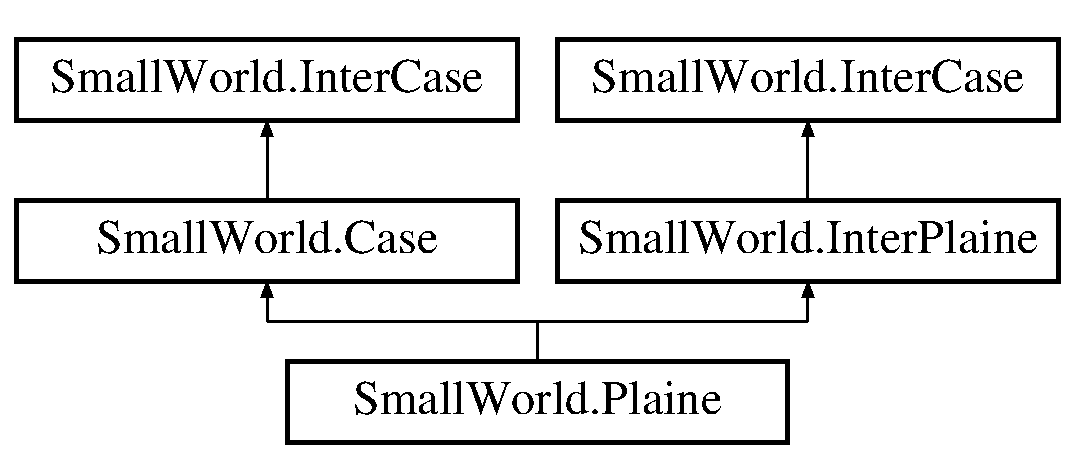
\includegraphics[height=3.000000cm]{class_small_world_1_1_plaine}
\end{center}
\end{figure}


\subsection{Detailed Description}
class pour \hyperlink{class_small_world_1_1_case}{Case} de type plaine 

The documentation for this class was generated from the following file\-:\begin{DoxyCompactItemize}
\item 
C\-:/\-Users/damienc/\-Documents/\-Git\-Hub/\-Small\-World/\-Visual\-Studio/\-Projet\-P\-O\-O/\hyperlink{_case_8cs}{Case.\-cs}\end{DoxyCompactItemize}

\hypertarget{class_small_world_1_1_strategie_carte}{\section{Small\-World.\-Strategie\-Carte Class Reference}
\label{class_small_world_1_1_strategie_carte}\index{Small\-World.\-Strategie\-Carte@{Small\-World.\-Strategie\-Carte}}
}


classe abstraite pour la stratégie  


Inheritance diagram for Small\-World.\-Strategie\-Carte\-:\begin{figure}[H]
\begin{center}
\leavevmode
\includegraphics[height=2.901554cm]{class_small_world_1_1_strategie_carte}
\end{center}
\end{figure}
\subsection*{Public Member Functions}
\begin{DoxyCompactItemize}
\item 
\hypertarget{class_small_world_1_1_strategie_carte_aafe89809c98196f4b1d48436d02bcbed}{unsafe List$<$ List$<$ \hyperlink{class_small_world_1_1_case}{Case} $>$ $>$ \hyperlink{class_small_world_1_1_strategie_carte_aafe89809c98196f4b1d48436d02bcbed}{construire} ()}\label{class_small_world_1_1_strategie_carte_aafe89809c98196f4b1d48436d02bcbed}

\begin{DoxyCompactList}\small\item\em Construit une nouvelle \hyperlink{class_small_world_1_1_carte}{Carte}. \end{DoxyCompactList}\end{DoxyCompactItemize}
\subsection*{Protected Attributes}
\begin{DoxyCompactItemize}
\item 
\hypertarget{class_small_world_1_1_strategie_carte_a04a14a2cc7b170caec54ff2d87f70724}{int \hyperlink{class_small_world_1_1_strategie_carte_a04a14a2cc7b170caec54ff2d87f70724}{taille}}\label{class_small_world_1_1_strategie_carte_a04a14a2cc7b170caec54ff2d87f70724}

\begin{DoxyCompactList}\small\item\em Attribut {\bfseries T\-A\-I\-L\-L\-E} indiquant la taille de la carte. \end{DoxyCompactList}\end{DoxyCompactItemize}
\subsection*{Properties}
\begin{DoxyCompactItemize}
\item 
\hypertarget{class_small_world_1_1_strategie_carte_ac0c543aa988e3c669cf5d9b17ea3cd31}{int \hyperlink{class_small_world_1_1_strategie_carte_ac0c543aa988e3c669cf5d9b17ea3cd31}{Taille}\hspace{0.3cm}{\ttfamily  \mbox{[}get\mbox{]}}}\label{class_small_world_1_1_strategie_carte_ac0c543aa988e3c669cf5d9b17ea3cd31}

\begin{DoxyCompactList}\small\item\em \hyperlink{namespace_small_world_1_1_properties}{Properties} pour l'attribut taille. \end{DoxyCompactList}\end{DoxyCompactItemize}


\subsection{Detailed Description}
classe abstraite pour la stratégie 

The documentation for this class was generated from the following file\-:\begin{DoxyCompactItemize}
\item 
C\-:/\-Users/damienc/\-Documents/\-Git\-Hub/\-Small\-World/\-Visual\-Studio/\-Projet\-P\-O\-O/\hyperlink{_strategie_8cs}{Strategie.\-cs}\end{DoxyCompactItemize}

\hypertarget{class_small_world_1_1_strategie_demo}{\section{Small\-World.\-Strategie\-Demo Class Reference}
\label{class_small_world_1_1_strategie_demo}\index{Small\-World.\-Strategie\-Demo@{Small\-World.\-Strategie\-Demo}}
}
Inheritance diagram for Small\-World.\-Strategie\-Demo\-:\begin{figure}[H]
\begin{center}
\leavevmode
\includegraphics[height=3.000000cm]{class_small_world_1_1_strategie_demo}
\end{center}
\end{figure}
\subsection*{Public Member Functions}
\begin{DoxyCompactItemize}
\item 
void \hyperlink{class_small_world_1_1_strategie_demo_a6a9bbb801d3f894d735dc21d9029c2ee}{construire} ()
\end{DoxyCompactItemize}


\subsection{Member Function Documentation}
\hypertarget{class_small_world_1_1_strategie_demo_a6a9bbb801d3f894d735dc21d9029c2ee}{\index{Small\-World\-::\-Strategie\-Demo@{Small\-World\-::\-Strategie\-Demo}!construire@{construire}}
\index{construire@{construire}!SmallWorld::StrategieDemo@{Small\-World\-::\-Strategie\-Demo}}
\subsubsection[{construire}]{\setlength{\rightskip}{0pt plus 5cm}void Small\-World.\-Strategie\-Demo.\-construire (
\begin{DoxyParamCaption}
{}
\end{DoxyParamCaption}
)}}\label{class_small_world_1_1_strategie_demo_a6a9bbb801d3f894d735dc21d9029c2ee}


Implements \hyperlink{interface_small_world_1_1_inter_strategie_demo_a58c028866f521ee3e50ea0d7e94268e7}{Small\-World.\-Inter\-Strategie\-Demo}.



The documentation for this class was generated from the following file\-:\begin{DoxyCompactItemize}
\item 
C\-:/\-Users/damienc/\-Documents/\-Git\-Hub/\-Small\-World/\-Visual\-Studio/\-Projet\-P\-O\-O/Strategie\-Demo.\-cs\end{DoxyCompactItemize}

\hypertarget{class_small_world_1_1_strategie_normale}{\section{Small\-World.\-Strategie\-Normale Class Reference}
\label{class_small_world_1_1_strategie_normale}\index{Small\-World.\-Strategie\-Normale@{Small\-World.\-Strategie\-Normale}}
}
Inheritance diagram for Small\-World.\-Strategie\-Normale\-:\begin{figure}[H]
\begin{center}
\leavevmode
\includegraphics[height=3.000000cm]{class_small_world_1_1_strategie_normale}
\end{center}
\end{figure}
\subsection*{Public Member Functions}
\begin{DoxyCompactItemize}
\item 
override void \hyperlink{class_small_world_1_1_strategie_normale_a8b9231f4b96f063008eeb670f8f09db6}{construire} ()
\end{DoxyCompactItemize}
\subsection*{Additional Inherited Members}


\subsection{Member Function Documentation}
\hypertarget{class_small_world_1_1_strategie_normale_a8b9231f4b96f063008eeb670f8f09db6}{\index{Small\-World\-::\-Strategie\-Normale@{Small\-World\-::\-Strategie\-Normale}!construire@{construire}}
\index{construire@{construire}!SmallWorld::StrategieNormale@{Small\-World\-::\-Strategie\-Normale}}
\subsubsection[{construire}]{\setlength{\rightskip}{0pt plus 5cm}override void Small\-World.\-Strategie\-Normale.\-construire (
\begin{DoxyParamCaption}
{}
\end{DoxyParamCaption}
)\hspace{0.3cm}{\ttfamily [virtual]}}}\label{class_small_world_1_1_strategie_normale_a8b9231f4b96f063008eeb670f8f09db6}


Implements \hyperlink{class_small_world_1_1_strategie_carte_a705ec27550d4dd65ec9295a851580c63}{Small\-World.\-Strategie\-Carte}.



The documentation for this class was generated from the following file\-:\begin{DoxyCompactItemize}
\item 
C\-:/\-Users/damienc/\-Documents/\-Git\-Hub/\-Small\-World/\-Visual\-Studio/\-Projet\-P\-O\-O/Strategie.\-cs\end{DoxyCompactItemize}

\hypertarget{class_small_world_1_1_strategie_petite}{\section{Small\-World.\-Strategie\-Petite Class Reference}
\label{class_small_world_1_1_strategie_petite}\index{Small\-World.\-Strategie\-Petite@{Small\-World.\-Strategie\-Petite}}
}
Inheritance diagram for Small\-World.\-Strategie\-Petite\-:\begin{figure}[H]
\begin{center}
\leavevmode
\includegraphics[height=3.000000cm]{class_small_world_1_1_strategie_petite}
\end{center}
\end{figure}
\subsection*{Public Member Functions}
\begin{DoxyCompactItemize}
\item 
override void \hyperlink{class_small_world_1_1_strategie_petite_a19e5824d046b8dc0e982465195458192}{construire} ()
\end{DoxyCompactItemize}
\subsection*{Additional Inherited Members}


\subsection{Member Function Documentation}
\hypertarget{class_small_world_1_1_strategie_petite_a19e5824d046b8dc0e982465195458192}{\index{Small\-World\-::\-Strategie\-Petite@{Small\-World\-::\-Strategie\-Petite}!construire@{construire}}
\index{construire@{construire}!SmallWorld::StrategiePetite@{Small\-World\-::\-Strategie\-Petite}}
\subsubsection[{construire}]{\setlength{\rightskip}{0pt plus 5cm}override void Small\-World.\-Strategie\-Petite.\-construire (
\begin{DoxyParamCaption}
{}
\end{DoxyParamCaption}
)\hspace{0.3cm}{\ttfamily [virtual]}}}\label{class_small_world_1_1_strategie_petite_a19e5824d046b8dc0e982465195458192}


Implements \hyperlink{class_small_world_1_1_strategie_carte_a705ec27550d4dd65ec9295a851580c63}{Small\-World.\-Strategie\-Carte}.



The documentation for this class was generated from the following file\-:\begin{DoxyCompactItemize}
\item 
C\-:/\-Users/damienc/\-Documents/\-Git\-Hub/\-Small\-World/\-Visual\-Studio/\-Projet\-P\-O\-O/Strategie.\-cs\end{DoxyCompactItemize}

\hypertarget{class_small_world_1_1_unite}{\section{Small\-World.\-Unite Class Reference}
\label{class_small_world_1_1_unite}\index{Small\-World.\-Unite@{Small\-World.\-Unite}}
}
Inheritance diagram for Small\-World.\-Unite\-:\begin{figure}[H]
\begin{center}
\leavevmode
\includegraphics[height=3.000000cm]{class_small_world_1_1_unite}
\end{center}
\end{figure}
\subsection*{Public Member Functions}
\begin{DoxyCompactItemize}
\item 
\hypertarget{class_small_world_1_1_unite_a5e792891c8194bd5344cf1d3a897226a}{void {\bfseries attaquer} ()}\label{class_small_world_1_1_unite_a5e792891c8194bd5344cf1d3a897226a}

\item 
\hypertarget{class_small_world_1_1_unite_a51ba4ffd6b0029b1cc7be453f47730c5}{void {\bfseries deplacer} ()}\label{class_small_world_1_1_unite_a51ba4ffd6b0029b1cc7be453f47730c5}

\end{DoxyCompactItemize}


The documentation for this class was generated from the following file\-:\begin{DoxyCompactItemize}
\item 
C\-:/\-Users/damienc/\-Documents/\-Git\-Hub/\-Small\-World/\-Visual\-Studio/\-Projet\-P\-O\-O/Unite.\-cs\end{DoxyCompactItemize}

\hypertarget{class_small_world_1_1_unite_gauloise}{\section{Small\-World.\-Unite\-Gauloise Class Reference}
\label{class_small_world_1_1_unite_gauloise}\index{Small\-World.\-Unite\-Gauloise@{Small\-World.\-Unite\-Gauloise}}
}
Inheritance diagram for Small\-World.\-Unite\-Gauloise\-:\begin{figure}[H]
\begin{center}
\leavevmode
\includegraphics[height=3.000000cm]{class_small_world_1_1_unite_gauloise}
\end{center}
\end{figure}
\subsection*{Additional Inherited Members}


The documentation for this class was generated from the following file\-:\begin{DoxyCompactItemize}
\item 
C\-:/\-Users/damienc/\-Documents/\-Git\-Hub/\-Small\-World/\-Visual\-Studio/\-Projet\-P\-O\-O/Unite\-Gauloise.\-cs\end{DoxyCompactItemize}

\hypertarget{class_small_world_1_1_unite_naine}{\section{Small\-World.\-Unite\-Naine Class Reference}
\label{class_small_world_1_1_unite_naine}\index{Small\-World.\-Unite\-Naine@{Small\-World.\-Unite\-Naine}}
}
Inheritance diagram for Small\-World.\-Unite\-Naine\-:\begin{figure}[H]
\begin{center}
\leavevmode
\includegraphics[height=3.000000cm]{class_small_world_1_1_unite_naine}
\end{center}
\end{figure}
\subsection*{Public Member Functions}
\begin{DoxyCompactItemize}
\item 
\hypertarget{class_small_world_1_1_unite_naine_acd80dd014d63ccccaa2743dfad1044d7}{void {\bfseries attaquer} ()}\label{class_small_world_1_1_unite_naine_acd80dd014d63ccccaa2743dfad1044d7}

\item 
\hypertarget{class_small_world_1_1_unite_naine_a2976f6b6d2bee701106717a69f6ff055}{void {\bfseries deplacer} ()}\label{class_small_world_1_1_unite_naine_a2976f6b6d2bee701106717a69f6ff055}

\end{DoxyCompactItemize}


The documentation for this class was generated from the following file\-:\begin{DoxyCompactItemize}
\item 
C\-:/\-Users/damienc/\-Documents/\-Git\-Hub/\-Small\-World/\-Visual\-Studio/\-Projet\-P\-O\-O/Unite\-Naine.\-cs\end{DoxyCompactItemize}

\hypertarget{class_small_world_1_1_unite_viking}{\section{Small\-World.\-Unite\-Viking Class Reference}
\label{class_small_world_1_1_unite_viking}\index{Small\-World.\-Unite\-Viking@{Small\-World.\-Unite\-Viking}}
}
Inheritance diagram for Small\-World.\-Unite\-Viking\-:\begin{figure}[H]
\begin{center}
\leavevmode
\includegraphics[height=3.000000cm]{class_small_world_1_1_unite_viking}
\end{center}
\end{figure}
\subsection*{Public Member Functions}
\begin{DoxyCompactItemize}
\item 
\hypertarget{class_small_world_1_1_unite_viking_acffa544aa9cc76789d2ba193884e3252}{void {\bfseries attaquer} ()}\label{class_small_world_1_1_unite_viking_acffa544aa9cc76789d2ba193884e3252}

\item 
\hypertarget{class_small_world_1_1_unite_viking_a9fbf828b2e54dfd2837340488b10817b}{void {\bfseries deplacer} ()}\label{class_small_world_1_1_unite_viking_a9fbf828b2e54dfd2837340488b10817b}

\end{DoxyCompactItemize}


The documentation for this class was generated from the following file\-:\begin{DoxyCompactItemize}
\item 
C\-:/\-Users/damienc/\-Documents/\-Git\-Hub/\-Small\-World/\-Visual\-Studio/\-Projet\-P\-O\-O/Unite\-Viking.\-cs\end{DoxyCompactItemize}

\chapter{File Documentation}
\hypertarget{_carte_8cs}{\section{C\-:/\-Users/damienc/\-Documents/\-Git\-Hub/\-Small\-World/\-Visual\-Studio/\-Projet\-P\-O\-O/\-Carte.cs File Reference}
\label{_carte_8cs}\index{C\-:/\-Users/damienc/\-Documents/\-Git\-Hub/\-Small\-World/\-Visual\-Studio/\-Projet\-P\-O\-O/\-Carte.\-cs@{C\-:/\-Users/damienc/\-Documents/\-Git\-Hub/\-Small\-World/\-Visual\-Studio/\-Projet\-P\-O\-O/\-Carte.\-cs}}
}


Interface et classe de la Carte.  


\subsection*{Classes}
\begin{DoxyCompactItemize}
\item 
interface \hyperlink{interface_small_world_1_1_inter_carte}{Small\-World.\-Inter\-Carte}
\begin{DoxyCompactList}\small\item\em Interface pour \hyperlink{class_small_world_1_1_carte}{Carte}. \end{DoxyCompactList}\item 
class \hyperlink{class_small_world_1_1_carte}{Small\-World.\-Carte}
\begin{DoxyCompactList}\small\item\em Classe \hyperlink{class_small_world_1_1_carte}{Carte} Représente la carte du monde. \end{DoxyCompactList}\end{DoxyCompactItemize}
\subsection*{Namespaces}
\begin{DoxyCompactItemize}
\item 
package \hyperlink{namespace_small_world}{Small\-World}
\end{DoxyCompactItemize}


\subsection{Detailed Description}
Interface et classe de la Carte. Une Carte représente le plateau de jeu et se compose d'un ensemble de Case, de type différent

\begin{DoxyAuthor}{Author}
\href{mailto:damien.cremilleux@insa-rennes.fr}{\tt Damien Crémilleux} 

\href{mailto:lauriane.holy@insa-rennes.fr}{\tt Lauriane Holy}
\end{DoxyAuthor}
\begin{DoxyDate}{Date}
15/01/2014 
\end{DoxyDate}
\begin{DoxyVersion}{Version}
0.\-1 
\end{DoxyVersion}

\hypertarget{_case_8cs}{\section{C\-:/\-Users/damienc/\-Documents/\-Git\-Hub/\-Small\-World/\-Visual\-Studio/\-Projet\-P\-O\-O/\-Case.cs File Reference}
\label{_case_8cs}\index{C\-:/\-Users/damienc/\-Documents/\-Git\-Hub/\-Small\-World/\-Visual\-Studio/\-Projet\-P\-O\-O/\-Case.\-cs@{C\-:/\-Users/damienc/\-Documents/\-Git\-Hub/\-Small\-World/\-Visual\-Studio/\-Projet\-P\-O\-O/\-Case.\-cs}}
}


Interfaces et classes pour les cases.  


\subsection*{Classes}
\begin{DoxyCompactItemize}
\item 
interface \hyperlink{interface_small_world_1_1_inter_case}{Small\-World.\-Inter\-Case}
\begin{DoxyCompactList}\small\item\em Interface pour \hyperlink{class_small_world_1_1_case}{Case}. \end{DoxyCompactList}\item 
interface \hyperlink{interface_small_world_1_1_inter_desert}{Small\-World.\-Inter\-Desert}
\begin{DoxyCompactList}\small\item\em Interface pour \hyperlink{class_small_world_1_1_case}{Case} de type désert. \end{DoxyCompactList}\item 
interface \hyperlink{interface_small_world_1_1_inter_eau}{Small\-World.\-Inter\-Eau}
\begin{DoxyCompactList}\small\item\em Interface pour \hyperlink{class_small_world_1_1_case}{Case} de type eau. \end{DoxyCompactList}\item 
interface \hyperlink{interface_small_world_1_1_inter_foret}{Small\-World.\-Inter\-Foret}
\begin{DoxyCompactList}\small\item\em Interface pour \hyperlink{class_small_world_1_1_case}{Case} de type forêt. \end{DoxyCompactList}\item 
interface \hyperlink{interface_small_world_1_1_inter_montagne}{Small\-World.\-Inter\-Montagne}
\begin{DoxyCompactList}\small\item\em Interface pour \hyperlink{class_small_world_1_1_case}{Case} de type montagne. \end{DoxyCompactList}\item 
interface \hyperlink{interface_small_world_1_1_inter_plaine}{Small\-World.\-Inter\-Plaine}
\begin{DoxyCompactList}\small\item\em Interface pour \hyperlink{class_small_world_1_1_case}{Case} de type plaine. \end{DoxyCompactList}\item 
class \hyperlink{class_small_world_1_1_case}{Small\-World.\-Case}
\begin{DoxyCompactList}\small\item\em classe abstraite \hyperlink{class_small_world_1_1_case}{Case} \end{DoxyCompactList}\item 
class \hyperlink{class_small_world_1_1_desert}{Small\-World.\-Desert}
\begin{DoxyCompactList}\small\item\em class pour \hyperlink{class_small_world_1_1_case}{Case} de type desert \end{DoxyCompactList}\item 
class \hyperlink{class_small_world_1_1_eau}{Small\-World.\-Eau}
\begin{DoxyCompactList}\small\item\em class pour \hyperlink{class_small_world_1_1_case}{Case} de type eau \end{DoxyCompactList}\item 
class \hyperlink{class_small_world_1_1_foret}{Small\-World.\-Foret}
\begin{DoxyCompactList}\small\item\em class pour \hyperlink{class_small_world_1_1_case}{Case} de type foret \end{DoxyCompactList}\item 
class \hyperlink{class_small_world_1_1_montagne}{Small\-World.\-Montagne}
\begin{DoxyCompactList}\small\item\em class pour \hyperlink{class_small_world_1_1_case}{Case} de type montagne \end{DoxyCompactList}\item 
class \hyperlink{class_small_world_1_1_plaine}{Small\-World.\-Plaine}
\begin{DoxyCompactList}\small\item\em class pour \hyperlink{class_small_world_1_1_case}{Case} de type plaine \end{DoxyCompactList}\end{DoxyCompactItemize}
\subsection*{Namespaces}
\begin{DoxyCompactItemize}
\item 
package \hyperlink{namespace_small_world}{Small\-World}
\end{DoxyCompactItemize}


\subsection{Detailed Description}
Interfaces et classes pour les cases. Les Cases sont les composants de la carte. Il en existe cinq types \-: désert, eau, forêt, montagne, plaine.

\begin{DoxyAuthor}{Author}
\href{mailto:damien.cremilleux@insa-rennes.fr}{\tt Damien Crémilleux} 

\href{mailto:lauriane.holy@insa-rennes.fr}{\tt Lauriane Holy}
\end{DoxyAuthor}
\begin{DoxyDate}{Date}
15/01/2014 
\end{DoxyDate}
\begin{DoxyVersion}{Version}
0.\-1 
\end{DoxyVersion}

\hypertarget{_constantes_8cs}{\section{C\-:/\-Users/damienc/\-Documents/\-Git\-Hub/\-Small\-World/\-Visual\-Studio/\-Projet\-P\-O\-O/\-Constantes.cs File Reference}
\label{_constantes_8cs}\index{C\-:/\-Users/damienc/\-Documents/\-Git\-Hub/\-Small\-World/\-Visual\-Studio/\-Projet\-P\-O\-O/\-Constantes.\-cs@{C\-:/\-Users/damienc/\-Documents/\-Git\-Hub/\-Small\-World/\-Visual\-Studio/\-Projet\-P\-O\-O/\-Constantes.\-cs}}
}


Constantes pour le jeu \hyperlink{namespace_small_world}{Small\-World}.  


\subsection*{Classes}
\begin{DoxyCompactItemize}
\item 
class \hyperlink{class_small_world_1_1_constantes}{Small\-World.\-Constantes}
\begin{DoxyCompactList}\small\item\em Les différentes constantes du jeu \hyperlink{namespace_small_world}{Small\-World}. \end{DoxyCompactList}\end{DoxyCompactItemize}
\subsection*{Namespaces}
\begin{DoxyCompactItemize}
\item 
package \hyperlink{namespace_small_world}{Small\-World}
\end{DoxyCompactItemize}


\subsection{Detailed Description}
Constantes pour le jeu \hyperlink{namespace_small_world}{Small\-World}. \begin{DoxyAuthor}{Author}
\href{mailto:damien.cremilleux@insa-rennes.fr}{\tt Damien Crémilleux} 

\href{mailto:lauriane.holy@insa-rennes.fr}{\tt Lauriane Holy}
\end{DoxyAuthor}
\begin{DoxyDate}{Date}
15/01/2014 
\end{DoxyDate}
\begin{DoxyVersion}{Version}
0.\-1 
\end{DoxyVersion}

\hypertarget{_coordonnees_8cs}{\section{C\-:/\-Users/damienc/\-Documents/\-Git\-Hub/\-Small\-World/\-Visual\-Studio/\-Projet\-P\-O\-O/\-Coordonnees.cs File Reference}
\label{_coordonnees_8cs}\index{C\-:/\-Users/damienc/\-Documents/\-Git\-Hub/\-Small\-World/\-Visual\-Studio/\-Projet\-P\-O\-O/\-Coordonnees.\-cs@{C\-:/\-Users/damienc/\-Documents/\-Git\-Hub/\-Small\-World/\-Visual\-Studio/\-Projet\-P\-O\-O/\-Coordonnees.\-cs}}
}


classe Coordonnees  


\subsection*{Classes}
\begin{DoxyCompactItemize}
\item 
interface \hyperlink{interface_small_world_1_1_inter_cordonnees}{Small\-World.\-Inter\-Cordonnees}
\item 
class \hyperlink{class_small_world_1_1_coordonnees}{Small\-World.\-Coordonnees}
\begin{DoxyCompactList}\small\item\em Rprésentation des coordonnées. \end{DoxyCompactList}\end{DoxyCompactItemize}
\subsection*{Namespaces}
\begin{DoxyCompactItemize}
\item 
package \hyperlink{namespace_small_world}{Small\-World}
\end{DoxyCompactItemize}


\subsection{Detailed Description}
classe Coordonnees Représentation de coordonnées pour le jeu \hyperlink{namespace_small_world}{Small\-World}

\begin{DoxyAuthor}{Author}
\href{mailto:damien.cremilleux@insa-rennes.fr}{\tt Damien Crémilleux} 

\href{mailto:lauriane.holy@insa-rennes.fr}{\tt Lauriane Holy}
\end{DoxyAuthor}
\begin{DoxyDate}{Date}
15/12/2013 
\end{DoxyDate}
\begin{DoxyVersion}{Version}
0.\-1 
\end{DoxyVersion}

\hypertarget{_createur_partie_8cs}{\section{C\-:/\-Users/damienc/\-Documents/\-Git\-Hub/\-Small\-World/\-Visual\-Studio/\-Projet\-P\-O\-O/\-Createur\-Partie.cs File Reference}
\label{_createur_partie_8cs}\index{C\-:/\-Users/damienc/\-Documents/\-Git\-Hub/\-Small\-World/\-Visual\-Studio/\-Projet\-P\-O\-O/\-Createur\-Partie.\-cs@{C\-:/\-Users/damienc/\-Documents/\-Git\-Hub/\-Small\-World/\-Visual\-Studio/\-Projet\-P\-O\-O/\-Createur\-Partie.\-cs}}
}


Interface et classe du créateur de partie.  


\subsection*{Classes}
\begin{DoxyCompactItemize}
\item 
interface \hyperlink{interface_small_world_1_1_inter_createur_partie}{Small\-World.\-Inter\-Createur\-Partie}
\begin{DoxyCompactList}\small\item\em Interface du créateur de partie. \end{DoxyCompactList}\item 
class \hyperlink{class_small_world_1_1_createur_partie}{Small\-World.\-Createur\-Partie}
\begin{DoxyCompactList}\small\item\em Class du créateur de partie. \end{DoxyCompactList}\end{DoxyCompactItemize}
\subsection*{Namespaces}
\begin{DoxyCompactItemize}
\item 
package \hyperlink{namespace_small_world}{Small\-World}
\end{DoxyCompactItemize}


\subsection{Detailed Description}
Interface et classe du créateur de partie. Directeur du patron de conception Monteur, contient le processus de création

\begin{DoxyAuthor}{Author}
\href{mailto:damien.cremilleux@insa-rennes.fr}{\tt Damien Crémilleux$<$/$>$  Lauriane Holy$<$/$>$  18/11/2013  0.\-1 }
\end{DoxyAuthor}

\hypertarget{_fabrique_case_8cs}{\section{C\-:/\-Users/damienc/\-Documents/\-Git\-Hub/\-Small\-World/\-Visual\-Studio/\-Projet\-P\-O\-O/\-Fabrique\-Case.cs File Reference}
\label{_fabrique_case_8cs}\index{C\-:/\-Users/damienc/\-Documents/\-Git\-Hub/\-Small\-World/\-Visual\-Studio/\-Projet\-P\-O\-O/\-Fabrique\-Case.\-cs@{C\-:/\-Users/damienc/\-Documents/\-Git\-Hub/\-Small\-World/\-Visual\-Studio/\-Projet\-P\-O\-O/\-Fabrique\-Case.\-cs}}
}


Fabrique pour les cases.  


\subsection*{Classes}
\begin{DoxyCompactItemize}
\item 
interface \hyperlink{interface_small_world_1_1_inter_fabrique_case}{Small\-World.\-Inter\-Fabrique\-Case}
\begin{DoxyCompactList}\small\item\em interface pour la fabrique de case \end{DoxyCompactList}\item 
class \hyperlink{class_small_world_1_1_fabrique_case}{Small\-World.\-Fabrique\-Case}
\begin{DoxyCompactList}\small\item\em classe \hyperlink{class_small_world_1_1_fabrique_case}{Fabrique\-Case} pour la génération de cases \end{DoxyCompactList}\end{DoxyCompactItemize}
\subsection*{Namespaces}
\begin{DoxyCompactItemize}
\item 
package \hyperlink{namespace_small_world}{Small\-World}
\end{DoxyCompactItemize}


\subsection{Detailed Description}
Fabrique pour les cases. Singleton pour fabriquer des cases, et utilisé dans le poids mouche

\begin{DoxyAuthor}{Author}
\href{mailto:damien.cremilleux@insa-rennes.fr}{\tt Damien Crémilleux} 

\href{mailto:lauriane.holy@insa-rennes.fr}{\tt Lauriane Holy}
\end{DoxyAuthor}
\begin{DoxyDate}{Date}
15/01/2014 
\end{DoxyDate}
\begin{DoxyVersion}{Version}
0.\-1 
\end{DoxyVersion}

\hypertarget{_fabrique_peuple_8cs}{\section{C\-:/\-Users/damienc/\-Documents/\-Git\-Hub/\-Small\-World/\-Visual\-Studio/\-Projet\-P\-O\-O/\-Fabrique\-Peuple.cs File Reference}
\label{_fabrique_peuple_8cs}\index{C\-:/\-Users/damienc/\-Documents/\-Git\-Hub/\-Small\-World/\-Visual\-Studio/\-Projet\-P\-O\-O/\-Fabrique\-Peuple.\-cs@{C\-:/\-Users/damienc/\-Documents/\-Git\-Hub/\-Small\-World/\-Visual\-Studio/\-Projet\-P\-O\-O/\-Fabrique\-Peuple.\-cs}}
}


Interfaces et classes pour la fabrique des peuples.  


\subsection*{Classes}
\begin{DoxyCompactItemize}
\item 
interface \hyperlink{interface_small_world_1_1_inter_fabrique_peuple}{Small\-World.\-Inter\-Fabrique\-Peuple}
\begin{DoxyCompactList}\small\item\em Interface pour la fabrique de peuple. \end{DoxyCompactList}\item 
class \hyperlink{class_small_world_1_1_fabrique_peuple}{Small\-World.\-Fabrique\-Peuple}
\begin{DoxyCompactList}\small\item\em classe pour la fabrique d'un peuple \end{DoxyCompactList}\end{DoxyCompactItemize}
\subsection*{Namespaces}
\begin{DoxyCompactItemize}
\item 
package \hyperlink{namespace_small_world}{Small\-World}
\end{DoxyCompactItemize}


\subsection{Detailed Description}
Interfaces et classes pour la fabrique des peuples. Fabrique des différents peuples \-: gaulois, nain, viking.

\begin{DoxyAuthor}{Author}
\href{mailto:damien.cremilleux@insa-rennes.fr}{\tt Damien Crémilleux} 

\href{mailto:lauriane.holy@insa-rennes.fr}{\tt Lauriane Holy}
\end{DoxyAuthor}
\begin{DoxyDate}{Date}
15/01/2014 
\end{DoxyDate}
\begin{DoxyVersion}{Version}
0.\-1 
\end{DoxyVersion}

\hypertarget{_joueur_8cs}{\section{C\-:/\-Users/damienc/\-Documents/\-Git\-Hub/\-Small\-World/\-Visual\-Studio/\-Projet\-P\-O\-O/\-Joueur.cs File Reference}
\label{_joueur_8cs}\index{C\-:/\-Users/damienc/\-Documents/\-Git\-Hub/\-Small\-World/\-Visual\-Studio/\-Projet\-P\-O\-O/\-Joueur.\-cs@{C\-:/\-Users/damienc/\-Documents/\-Git\-Hub/\-Small\-World/\-Visual\-Studio/\-Projet\-P\-O\-O/\-Joueur.\-cs}}
}


Interface et classe pour les joueurs.  


\subsection*{Classes}
\begin{DoxyCompactItemize}
\item 
interface \hyperlink{interface_small_world_1_1_inter_joueur}{Small\-World.\-Inter\-Joueur}
\begin{DoxyCompactList}\small\item\em interface pour un joueur \end{DoxyCompactList}\item 
class \hyperlink{class_small_world_1_1_joueur}{Small\-World.\-Joueur}
\begin{DoxyCompactList}\small\item\em classe pour un joueur \end{DoxyCompactList}\end{DoxyCompactItemize}
\subsection*{Namespaces}
\begin{DoxyCompactItemize}
\item 
package \hyperlink{namespace_small_world}{Small\-World}
\end{DoxyCompactItemize}


\subsection{Detailed Description}
Interface et classe pour les joueurs. Participants au jeu \hyperlink{namespace_small_world}{Small\-World}

\begin{DoxyAuthor}{Author}
\href{mailto:damien.cremilleux@insa-rennes.fr}{\tt Damien Crémilleux} 

\href{mailto:lauriane.holy@insa-rennes.fr}{\tt Lauriane Holy}
\end{DoxyAuthor}
\begin{DoxyDate}{Date}
15/01/2014 
\end{DoxyDate}
\begin{DoxyVersion}{Version}
0.\-1 
\end{DoxyVersion}

\hypertarget{_monteur_partie_8cs}{\section{C\-:/\-Users/damienc/\-Documents/\-Git\-Hub/\-Small\-World/\-Visual\-Studio/\-Projet\-P\-O\-O/\-Monteur\-Partie.cs File Reference}
\label{_monteur_partie_8cs}\index{C\-:/\-Users/damienc/\-Documents/\-Git\-Hub/\-Small\-World/\-Visual\-Studio/\-Projet\-P\-O\-O/\-Monteur\-Partie.\-cs@{C\-:/\-Users/damienc/\-Documents/\-Git\-Hub/\-Small\-World/\-Visual\-Studio/\-Projet\-P\-O\-O/\-Monteur\-Partie.\-cs}}
}


Interfaces et classes du monteur de partie.  


\subsection*{Classes}
\begin{DoxyCompactItemize}
\item 
interface \hyperlink{interface_small_world_1_1_inter_monteur_partie}{Small\-World.\-Inter\-Monteur\-Partie}
\begin{DoxyCompactList}\small\item\em Interface globale du monteur. \end{DoxyCompactList}\item 
interface \hyperlink{interface_small_world_1_1_inter_monteur_partie_demo}{Small\-World.\-Inter\-Monteur\-Partie\-Demo}
\begin{DoxyCompactList}\small\item\em Interface du monteur de partie démo. \end{DoxyCompactList}\item 
interface \hyperlink{interface_small_world_1_1_inter_monteur_partie_petite}{Small\-World.\-Inter\-Monteur\-Partie\-Petite}
\begin{DoxyCompactList}\small\item\em Interface du monteur de partie petite. \end{DoxyCompactList}\item 
interface \hyperlink{interface_small_world_1_1_inter_monteur_partie_normale}{Small\-World.\-Inter\-Monteur\-Partie\-Normale}
\begin{DoxyCompactList}\small\item\em Interface du monteur de partie normale. \end{DoxyCompactList}\item 
class \hyperlink{class_small_world_1_1_monteur_partie}{Small\-World.\-Monteur\-Partie}
\begin{DoxyCompactList}\small\item\em Classe abstraite implémentant Inter\-Monteur \hyperlink{interface_small_world_1_1_inter_partie}{Inter\-Partie}. \end{DoxyCompactList}\item 
class \hyperlink{class_small_world_1_1_monteur_partie_demo}{Small\-World.\-Monteur\-Partie\-Demo}
\begin{DoxyCompactList}\small\item\em classe pour un monteur d'une partie démo \end{DoxyCompactList}\item 
class \hyperlink{class_small_world_1_1_monteur_partie_petite}{Small\-World.\-Monteur\-Partie\-Petite}
\begin{DoxyCompactList}\small\item\em classe pour un monteur d'une partie petite \end{DoxyCompactList}\item 
class \hyperlink{class_small_world_1_1_monteur_partie_normale}{Small\-World.\-Monteur\-Partie\-Normale}
\begin{DoxyCompactList}\small\item\em classe pour un monteur d'une partie normale \end{DoxyCompactList}\end{DoxyCompactItemize}
\subsection*{Namespaces}
\begin{DoxyCompactItemize}
\item 
package \hyperlink{namespace_small_world}{Small\-World}
\end{DoxyCompactItemize}


\subsection{Detailed Description}
Interfaces et classes du monteur de partie. Monteur du patron de conception monteur, contient les interfaces et les différentes implémentations pour le processus de création d'une partie

\begin{DoxyAuthor}{Author}
\href{mailto:damien.cremilleux@insa-rennes.fr}{\tt Damien Crémilleux} 

\href{mailto:lauriane.holy@insa-rennes.fr}{\tt Lauriane Holy}
\end{DoxyAuthor}
\begin{DoxyDate}{Date}
15/01/2014 
\end{DoxyDate}
\begin{DoxyVersion}{Version}
0.\-1 
\end{DoxyVersion}

\hypertarget{_partie_8cs}{\section{C\-:/\-Users/damienc/\-Documents/\-Git\-Hub/\-Small\-World/\-Visual\-Studio/\-Projet\-P\-O\-O/\-Partie.cs File Reference}
\label{_partie_8cs}\index{C\-:/\-Users/damienc/\-Documents/\-Git\-Hub/\-Small\-World/\-Visual\-Studio/\-Projet\-P\-O\-O/\-Partie.\-cs@{C\-:/\-Users/damienc/\-Documents/\-Git\-Hub/\-Small\-World/\-Visual\-Studio/\-Projet\-P\-O\-O/\-Partie.\-cs}}
}


Interface et classe d'une partie.  


\subsection*{Classes}
\begin{DoxyCompactItemize}
\item 
interface \hyperlink{interface_small_world_1_1_inter_partie}{Small\-World.\-Inter\-Partie}
\begin{DoxyCompactList}\small\item\em interface pour les partie \end{DoxyCompactList}\item 
class \hyperlink{class_small_world_1_1_partie}{Small\-World.\-Partie}
\begin{DoxyCompactList}\small\item\em classe pour les parties \end{DoxyCompactList}\end{DoxyCompactItemize}
\subsection*{Namespaces}
\begin{DoxyCompactItemize}
\item 
package \hyperlink{namespace_small_world}{Small\-World}
\end{DoxyCompactItemize}


\subsection{Detailed Description}
Interface et classe d'une partie. \begin{DoxyAuthor}{Author}
\href{mailto:damien.cremilleux@insa-rennes.fr}{\tt Damien Crémilleux} 

\href{mailto:lauriane.holy@insa-rennes.fr}{\tt Lauriane Holy}
\end{DoxyAuthor}
\begin{DoxyDate}{Date}
15/01/2014 
\end{DoxyDate}
\begin{DoxyVersion}{Version}
0.\-1 
\end{DoxyVersion}

\hypertarget{_peuple_8cs}{\section{C\-:/\-Users/damienc/\-Documents/\-Git\-Hub/\-Small\-World/\-Visual\-Studio/\-Projet\-P\-O\-O/\-Peuple.cs File Reference}
\label{_peuple_8cs}\index{C\-:/\-Users/damienc/\-Documents/\-Git\-Hub/\-Small\-World/\-Visual\-Studio/\-Projet\-P\-O\-O/\-Peuple.\-cs@{C\-:/\-Users/damienc/\-Documents/\-Git\-Hub/\-Small\-World/\-Visual\-Studio/\-Projet\-P\-O\-O/\-Peuple.\-cs}}
}


Interface et classe pour les peuples.  


\subsection*{Classes}
\begin{DoxyCompactItemize}
\item 
interface \hyperlink{interface_small_world_1_1_inter_peuple}{Small\-World.\-Inter\-Peuple}
\begin{DoxyCompactList}\small\item\em interface globale pour les peuples \end{DoxyCompactList}\item 
class \hyperlink{class_small_world_1_1_peuple}{Small\-World.\-Peuple}
\begin{DoxyCompactList}\small\item\em classe abstraite pour les peuples \end{DoxyCompactList}\item 
interface \hyperlink{interface_small_world_1_1_inter_peuple_gaulois}{Small\-World.\-Inter\-Peuple\-Gaulois}
\begin{DoxyCompactList}\small\item\em interface pour le peuple gaulois \end{DoxyCompactList}\item 
interface \hyperlink{interface_small_world_1_1_inter_peuple_nain}{Small\-World.\-Inter\-Peuple\-Nain}
\begin{DoxyCompactList}\small\item\em interface pour le peuple nain \end{DoxyCompactList}\item 
interface \hyperlink{interface_small_world_1_1_inter_peuple_viking}{Small\-World.\-Inter\-Peuple\-Viking}
\begin{DoxyCompactList}\small\item\em interface pour le peuple viking \end{DoxyCompactList}\item 
class \hyperlink{class_small_world_1_1_peuple_gaulois}{Small\-World.\-Peuple\-Gaulois}
\begin{DoxyCompactList}\small\item\em classe pour le peuple Gaulois \end{DoxyCompactList}\item 
class \hyperlink{class_small_world_1_1_peuple_nain}{Small\-World.\-Peuple\-Nain}
\begin{DoxyCompactList}\small\item\em classe pour le peuple nain \end{DoxyCompactList}\item 
class \hyperlink{class_small_world_1_1_peuple_viking}{Small\-World.\-Peuple\-Viking}
\begin{DoxyCompactList}\small\item\em classe pour le peuple viking \end{DoxyCompactList}\end{DoxyCompactItemize}
\subsection*{Namespaces}
\begin{DoxyCompactItemize}
\item 
package \hyperlink{namespace_small_world}{Small\-World}
\end{DoxyCompactItemize}


\subsection{Detailed Description}
Interface et classe pour les peuples. Chaque joueur est d'un peuple particulier.

\begin{DoxyAuthor}{Author}
\href{mailto:damien.cremilleux@insa-rennes.fr}{\tt Damien Crémilleux} 

\href{mailto:lauriane.holy@insa-rennes.fr}{\tt Lauriane Holy}
\end{DoxyAuthor}
\begin{DoxyDate}{Date}
15/01/2014 
\end{DoxyDate}
\begin{DoxyVersion}{Version}
0.\-1 
\end{DoxyVersion}

\hypertarget{_strategie_8cs}{\section{C\-:/\-Users/damienc/\-Documents/\-Git\-Hub/\-Small\-World/\-Visual\-Studio/\-Projet\-P\-O\-O/\-Strategie.cs File Reference}
\label{_strategie_8cs}\index{C\-:/\-Users/damienc/\-Documents/\-Git\-Hub/\-Small\-World/\-Visual\-Studio/\-Projet\-P\-O\-O/\-Strategie.\-cs@{C\-:/\-Users/damienc/\-Documents/\-Git\-Hub/\-Small\-World/\-Visual\-Studio/\-Projet\-P\-O\-O/\-Strategie.\-cs}}
}


Interface et classe pour le patron de coneption stratégie.  


\subsection*{Classes}
\begin{DoxyCompactItemize}
\item 
interface \hyperlink{interface_small_world_1_1_inter_strategie_carte}{Small\-World.\-Inter\-Strategie\-Carte}
\begin{DoxyCompactList}\small\item\em interface globale pour la stratégie \end{DoxyCompactList}\item 
class \hyperlink{class_small_world_1_1_strategie_carte}{Small\-World.\-Strategie\-Carte}
\begin{DoxyCompactList}\small\item\em classe abstraite pour la stratégie \end{DoxyCompactList}\item 
interface \hyperlink{interface_small_world_1_1_inter_strategie_demo}{Small\-World.\-Inter\-Strategie\-Demo}
\begin{DoxyCompactList}\small\item\em interface pour une stratégie démo \end{DoxyCompactList}\item 
interface \hyperlink{interface_small_world_1_1_inter_strategie_petite}{Small\-World.\-Inter\-Strategie\-Petite}
\begin{DoxyCompactList}\small\item\em interface pour une stratégie petite \end{DoxyCompactList}\item 
interface \hyperlink{interface_small_world_1_1_inter_strategie_normale}{Small\-World.\-Inter\-Strategie\-Normale}
\begin{DoxyCompactList}\small\item\em interface pour une stratégie normale \end{DoxyCompactList}\item 
class \hyperlink{class_small_world_1_1_strategie_demo}{Small\-World.\-Strategie\-Demo}
\begin{DoxyCompactList}\small\item\em classe pour une stratégie démo \end{DoxyCompactList}\item 
class \hyperlink{class_small_world_1_1_strategie_petite}{Small\-World.\-Strategie\-Petite}
\begin{DoxyCompactList}\small\item\em classe pour une stratégie petite \end{DoxyCompactList}\item 
class \hyperlink{class_small_world_1_1_strategie_normale}{Small\-World.\-Strategie\-Normale}
\begin{DoxyCompactList}\small\item\em classe pour une stratégie normale \end{DoxyCompactList}\end{DoxyCompactItemize}
\subsection*{Namespaces}
\begin{DoxyCompactItemize}
\item 
package \hyperlink{namespace_small_world}{Small\-World}
\end{DoxyCompactItemize}


\subsection{Detailed Description}
Interface et classe pour le patron de coneption stratégie. \begin{DoxyAuthor}{Author}
\href{mailto:damien.cremilleux@insa-rennes.fr}{\tt Damien Crémilleux} 

\href{mailto:lauriane.holy@insa-rennes.fr}{\tt Lauriane Holy}
\end{DoxyAuthor}
\begin{DoxyDate}{Date}
15/01/2014 
\end{DoxyDate}
\begin{DoxyVersion}{Version}
0.\-1 
\end{DoxyVersion}

\hypertarget{_unite_8cs}{\section{C\-:/\-Users/damienc/\-Documents/\-Git\-Hub/\-Small\-World/\-Visual\-Studio/\-Projet\-P\-O\-O/\-Unite.cs File Reference}
\label{_unite_8cs}\index{C\-:/\-Users/damienc/\-Documents/\-Git\-Hub/\-Small\-World/\-Visual\-Studio/\-Projet\-P\-O\-O/\-Unite.\-cs@{C\-:/\-Users/damienc/\-Documents/\-Git\-Hub/\-Small\-World/\-Visual\-Studio/\-Projet\-P\-O\-O/\-Unite.\-cs}}
}


Interface et classe pour les unités.  


\subsection*{Classes}
\begin{DoxyCompactItemize}
\item 
interface \hyperlink{interface_small_world_1_1_inter_unite}{Small\-World.\-Inter\-Unite}
\begin{DoxyCompactList}\small\item\em interface pour les unités \end{DoxyCompactList}\item 
interface \hyperlink{interface_small_world_1_1_inter_unite_gauloise}{Small\-World.\-Inter\-Unite\-Gauloise}
\begin{DoxyCompactList}\small\item\em Interface pour les unités gauloises. \end{DoxyCompactList}\item 
interface \hyperlink{interface_small_world_1_1_inter_unite_naine}{Small\-World.\-Inter\-Unite\-Naine}
\begin{DoxyCompactList}\small\item\em Interface pour les unités naines. \end{DoxyCompactList}\item 
interface \hyperlink{interface_small_world_1_1_inter_unite_viking}{Small\-World.\-Inter\-Unite\-Viking}
\begin{DoxyCompactList}\small\item\em Interface pour les unités viking. \end{DoxyCompactList}\item 
class \hyperlink{class_small_world_1_1_unite}{Small\-World.\-Unite}
\begin{DoxyCompactList}\small\item\em Classe abstraite pour les unités. \end{DoxyCompactList}\item 
class \hyperlink{class_small_world_1_1_unite_gauloise}{Small\-World.\-Unite\-Gauloise}
\begin{DoxyCompactList}\small\item\em Classe pour les unités gauloises. \end{DoxyCompactList}\item 
class \hyperlink{class_small_world_1_1_unite_naine}{Small\-World.\-Unite\-Naine}
\begin{DoxyCompactList}\small\item\em Classe pour les unités naines. \end{DoxyCompactList}\item 
class \hyperlink{class_small_world_1_1_unite_viking}{Small\-World.\-Unite\-Viking}
\begin{DoxyCompactList}\small\item\em Classe pour les unités viking. \end{DoxyCompactList}\end{DoxyCompactItemize}
\subsection*{Namespaces}
\begin{DoxyCompactItemize}
\item 
package \hyperlink{namespace_small_world}{Small\-World}
\end{DoxyCompactItemize}


\subsection{Detailed Description}
Interface et classe pour les unités. Les unités sont déplacés par les joueurs. Selon le peuple, les unités ont des caractéristiques différentes.

\begin{DoxyAuthor}{Author}
\href{mailto:damien.cremilleux@insa-rennes.fr}{\tt Damien Crémilleux} 

\href{mailto:lauriane.holy@insa-rennes.fr}{\tt Lauriane Holy}
\end{DoxyAuthor}
\begin{DoxyDate}{Date}
15/01/2014 
\end{DoxyDate}
\begin{DoxyVersion}{Version}
0.\-1 
\end{DoxyVersion}

%--- End generated contents ---

% Index
\newpage
\phantomsection
\addcontentsline{toc}{part}{Index}
\printindex

\end{document}
